\section{Design of UV Raman experiment}

Work on the construction of a new UV Raman spectrometer was an incremental
process.
It was necessary to consider the equipment already present in the lab, mainly
the laser system, CCD camera, and optical table and specify parameters of the
chosen commercial spectrograph.
Then the first functional prototype was constructed and improved for
measurement of polarized UV Raman spectra.
The initial wavenumber calibration technique of measured Raman spectra
was adopted based on the literature.
Then we started to deal with photo-decomposition of samples by designing a
spinning cell that could contain as small as cca. 20\,\g{m}l volumes of
samples.
After that, we widened the range of usable excitation wavelengths of the
instrument and decided to seek a new means of wavenumber calibration, and
after some research and trials and errors, we settled with calibration to the
spectra of Pt lamp.
And then, the apparatus was enhanced to enable temperature measurements in
backscattering geometry.
Next sections describe each step of the development of the UV Raman
spectrometer in more details.

\subsection{Initial equipment}
\label{initial_equipment}

As an excitation source, we used the Coherent Innova 300C
MotoFreD\texttrademark{} Ion Laser which enables intracavity frequency
doubling~\parencite{Asher1993b} of fundamental Ar ion emission lines by
nonlinear crystal. As a frequency doubling crystal we used BBO crystal (also
from Coherent) designed for doubling 488\,nm. Later we extended our
experimental options with additional two crystals designed for doubling 514 and
457\,nm. The BBO crystals are hygroscopic so they needed to be purged by steady
flow of 0.25--0.5 l/min of dry nitrogen of at least grade 5 purity (99.999\%)
\CITATION(laser manual). As a source of this nitrogen we decided to use
nitrogen generator NG1/1 from Gas Generation LTD which uses the pressure
swing absorption technology.

The above mentioned crystals could be used for
frequency doubling also the adjacent Ar ion lines. All the frequency doubled
wavelengths and expected and measured output laser beam powers which we could
tune with these three crystals are listed in
\tabref{initial_equipment:laser_power_spec}. The output wavelengths were
measured with HighFinesse High Precision Wavelength Meter WS5 UV-II and output
powers were measured with Power Meter from Thorlabs. The output powers in the
table were somewhat maximal which we could achieve, usually the power was
lower depending on laser condition. The 264.342\,nm wavelength was not possible
with our laser configuration because we couldn't tune the fundamental
528.693\,nm laser line for visible operation.

\begin{table}
	\centering
	\newcommand*{\nodotcell}[1]{\multicolumn{1}{r@{\hphantom{.}}}{#1}}

\begin{tabular}{c@{\hspace{5mm}}r@{\hspace{7mm}}>{\hspace{6mm}}r@{.}l}
\toprule
$\lambda$ (nm) & \multicolumn{1}{c}{$P_\text{e}$ (mW)}
                     & \multicolumn{2}{c}{$P_\text{m}$ (mW)} \\
\midrule

228.962        &  10 &              2&37 \\
238.238        &  30 &             33&5  \\
243.989        & 100 & \nodotcell{110}   \\
248.250        &  60 &             33&2  \\
250.854        &  15 &             11&4  \\
257.261        & 100 & \nodotcell{170}   \\

\bottomrule
\end{tabular}

	\caption{Specifications of laser power of frequency doubled lines.
	$P_\text{e}$ denotes expected laser power and $P_\text{m}$ measured
	laser powers. The wavelengths are measured in air at $20\,^\circ$C.}
	\label{\tablabel{initial_equipment:laser_power_spec}}
\end{table}

As a detector, we used liquid nitrogen cooled Princeton Instruments
SPEC-10:2KBUV/LN backiluminated CCD camera enhanced for UV light detection.
The camera has $2048\times512$ pixels of $13.5\times13.5$\,\g{m}m and can
be controlled with WinSpec software through ST133B/U camera controller unit.

\subsection{Choice of spectrograph parameters}
\begin{docitemize}
	\item Introduce dispersion according to focal length and groove density of
	grating.
	\begin{docitemize}
		\item How the theoretical values were computed using theoretical dispersion
			from Horiba manual.
		\item How the experimental values were measured and how we extrapolated
			for possible new grating selection
	\end{docitemize}
	\item Produce table of possible scenarios:
	\begin{docitemize}
		\item Theoretical values \tabref{spectrograph_selection:dispersion_theory}
		\item Experimental values
	\end{docitemize}
	\item Present decision criteria.
\end{docitemize}


\begin{table}
	\centering
	\begin{tabular}{crrrrrrrr}
\toprule
$\lambda$ (nm)
    & grating & 1200 & \multicolumn{2}{c}{1800}
        & \multicolumn{2}{c}{2400} & \multicolumn{2}{c}{3600} \\
\midrule
\multirow{3}{*}{228.962}
    & lower &   200 &   200 &   131 &   200 &  1551 &   200 &  3291 \\
    & upper &  6231 &  4057 &  4000 &  2804 &  4000 &  1020 &  4000 \\
    & disp. & 2.945 & 1.883 & 1.889 & 1.271 & 1.196 & 0.401 & 0.346 \\
\midrule
\multirow{3}{*}{238.238}
    & lower &   200 &   200 &   470 &   200 &  1762 &   200 &  3351 \\
    & upper &  5799 &  3774 &  4000 &  2610 &  4000 &   958 &  4000 \\
    & disp. & 2.734 & 1.745 & 1.723 & 1.177 & 1.093 & 0.370 & 0.317 \\
\midrule
\multirow{3}{*}{243.989}
    & lower &   200 &   200 &   660 &   200 &  1881 &   200 &  3385 \\
    & upper &  5554 &  3613 &  4000 &  2500 &  4000 &   923 &  4000 \\
    & disp. & 2.614 & 1.667 & 1.631 & 1.123 & 1.035 & 0.353 & 0.300 \\
\midrule
\multirow{3}{*}{248.250}
    & lower &   200 &   200 &   791 &   200 &  1963 &   200 &  3408 \\
    & upper &  5382 &  3502 &  4000 &  2424 &  4000 &   898 &  4000 \\
    & disp. & 2.531 & 1.612 & 1.567 & 1.086 & 0.995 & 0.341 & 0.289 \\
\midrule
\multirow{3}{*}{250.854}
    & lower &   200 &   200 &   868 &   200 &  2011 &   200 &  3422 \\
    & upper &  5282 &  3436 &  4000 &  2379 &  4000 &   884 &  4000 \\
    & disp. & 2.481 & 1.580 & 1.529 & 1.064 & 0.971 & 0.334 & 0.282 \\
\midrule
\multirow{3}{*}{257.261}
    & lower &   200 &   200 &  1046 &   200 &  2122 &   200 &  3454 \\
    & upper &  5046 &  3282 &  4000 &  2274 &  4000 &   850 &  4000 \\
    & disp. & 2.366 & 1.505 & 1.442 & 1.013 & 0.917 & 0.318 & 0.267 \\
\midrule
\multirow{3}{*}{264.345}
    & lower &   200 &   200 &  1227 &   200 &  2236 &   200 &  3486 \\
    & upper &  4804 &  3125 &  4000 &  2166 &  4000 &   816 &  4000 \\
    & disp. & 2.248 & 1.428 & 1.354 & 0.960 & 0.862 & 0.301 & 0.251 \\
\bottomrule
\end{tabular}

	\caption{Spectrograph dispersion -- theory. Gratins are denoted by number
		of grooves per mm, lowest and highest mean the lowest and highest detected
		frequency in \icm, respectively. The disp. denotes average dispersion in
		\icm/px.}
	\label{\tablabel{spectrograph_selection:dispersion_theory}}
\end{table}

Finaly, we chose grating with 300 gr/mm for possible fluorescence measurements
1200 gr/mm for the measurement of full range including valence hydrogen
stretching vibrations at higher wavelengths (e.g. 257\,nm excitation) and
2400 gr/mm for the most precise measurements.
\subsection{Initial layout of the instrument}

At first, we built a proof of concept apparatus to test if we selected the
right optical elements. Optical schema is depicted in
\figref{initial_layout:apparatus_schema}.
The laser beam is emitted with horizontal polarization and we decided, that we
want to guide it through a sample in vertical direction and gather the
scattered light in right angle geometry. Because of the steric restrictions in
our laboratory we needed to place the laser in such a way that it produced
laser beam in the oposit direction then we gathered the scattered light.
Because of that we needed to guide the beam in the loop using laser mirrors
enhanced for 244\,nm \emph{M1} and \emph{M2} (Thorlabs) to maintain the right
polarization direction because we wanted to be able to measure not only
depolarized Raman spectra. The beam was then turned up by another laser mirror
enhanced for 244\,nm \emph{M3} and hit the bottom of the sample cell, having
polarization perpendicular to the direction of scattered signal acquisition.
The excitation beam was focused onto the sample by the plano-convex lens
\emph{L1} with focal length 100\,mm. The most practical place for this lens
was between M2 and M3 so we couldn't select shorter focal length as is proposed
in \cref{subsec:focus_optimization}. The excitation laser beam could be attenuated by
the neutral density filters \emph{ND} with selection of 0.5, 1, 2, 3 and 4
optical densities (Thorlabs) which were placed inside carousel (Thorlabs) for
easy switching. We also old single blade shutter which we found in our
laboratory. The shutter was controlled from the CCD port for external shutter
by the WinSpec software provided with the detector. We needed to insert
condenser into the path because the leading edge of output signal from CCD was
too sharp. The shutter was open during measurement and closed rest of the time
to prevent photodecomposition of samples by the UV laser beam.

\begin{figure}
	\centering
	\begin{tikzpicture}[font=\sffamily]

% settings
\newcommand*{\cellBorderWidth}{3\pgflinewidth}
\newcommand*{\cellLineWidth}{1.5\pgflinewidth}
\definecolor{glassBorderColor}{RGB}{0,128,255}
\definecolor{glassFillColor}{RGB}{230,242,255}
\definecolor{waterFillColor}{RGB}{0,128,255}
\tikzset{
	clip
}
\tikzset{
	mirror element/.style={color=black, line width=2*\pgflinewidth},
	laser beam/.style={color=cyan, line width=2*\pgflinewidth},
	scattered ray/.style={color=red!60, line width=1.5*\pgflinewidth},
	scattered fill/.style={fill=red, draw=none, fill opacity=0.2},
	glass/.style={color=glassBorderColor, opacity=0.5,%
		fill=glassFillColor, fill opacity=0.5},
	sample cell/.style={color=glassBorderColor, opacity=0.5,%
		double=glassFillColor, double distance=\cellBorderWidth,
		line width=\cellLineWidth, line cap=rect},
	water fill/.style={fill=waterFillColor, fill opacity=0.1},
	mirror surface/.style={color=black!20, fill=black!10},
	nd filter/.style={color=black, opacity=0.2, fill=black, fill opacity=0.1},
	nd carousel/.style={color=black, opacity=0.4, fill=black, fill opacity=0.2},
	notch/.style={color=black, opacity=0.4, fill=black, fill opacity=0.1},
	aperture/.style={color=black, line width=2*\pgflinewidth},
	aperture filldraw/.style={color=black!40, fill=black!20, clip even odd rule},
	clip even odd rule/.code={\pgfseteorule},
	shutter/.style={nd carousel},
	shutter blade/.style={dashed, line width = 1.5*\pgflinewidth, opacity = 0.4}
};
\clip (-.1,-2.1) rectangle (14,6.6);
\coordinate (shutter) at (11,6);
\newcommand*{\samplePosWidth}{10}
\newcommand*{\samplePosHeight}{3}
\coordinate (samplePos) at (\samplePosWidth,\samplePosHeight);
\newcommand*{\cellWidth}{1};
\coordinate (cassegrainM1Center) at (\samplePosWidth - 0.5,\samplePosHeight);
\newcommand*{\cassegrainMARadius}{1.5}
\coordinate (cassegrainM2Center) at (\samplePosWidth - 0.7,\samplePosHeight);
\newcommand*{\cassegrainMBRadius}{0.4}
\newcommand*{\sqrttwo}{1.414213}
\coordinate (MS1Edge1) at (4.5,\samplePosHeight + 0.5);
\coordinate (MS1Edge2) at (3.5,\samplePosHeight - 0.5);
\coordinate (parabolaFocus) at (3,0.4);
\coordinate (MS2Edge1) at (4.5,1);
\coordinate (MS2EdgeControl1) at (245:0.5);
\coordinate (MS2Edge2) at (3.5,0);
\coordinate (MS2EdgeControl2) at (17:0.3);
\newcommand*{\apertureOuterRadius}{0.3}
\newcommand*{\apertureInnerRadius}{0.1}

% laser
\draw (0,5.5) rectangle ++(3,1) node[pos=.5] {laser};

% Mirror 3 - it should be under the beam so we have to draw it first
\draw[mirror surface] ($ (samplePos) + (-0.3,-\sqrttwo * 0.3) $)
	rectangle ++(0.6,\sqrttwo*0.6);
\node[above] at ($ (samplePos) + (0,0.5) $) {M3};

% laser beam
\draw[laser beam] (3,6) -- (13,6) coordinate (M1)
	-- (13,\samplePosHeight) coordinate (M2) -- (samplePos);

% aperture 2
\draw[aperture filldraw]
	(samplePos) circle (\apertureOuterRadius)
	(samplePos) circle (\apertureInnerRadius);

% neutral density filters
\newcommand*{\ndfilterA}{(3.5,5.8) rectangle ++(0.2,0.4)}
\newcommand*{\ndfilterB}{(3.5,5) rectangle ++(0.2,0.4)}
\draw[nd filter] \ndfilterA;
\draw[nd filter] \ndfilterB;
\draw[nd carousel] (3.45,4.9) rectangle ++(0.3,0.1);
\draw[nd carousel] (3.45,5.4) rectangle ++(0.3,0.4);
\draw[nd carousel] (3.45,6.2) rectangle ++(0.3,0.1);
\node[below] at (3.6,4.9) {ND};

\draw[shutter blade] ($ (shutter) + (0,0.3) $) -- ++(0,-0.6);
\draw[shutter] ($ (shutter) + (-0.1,-0.3) $) -- ++(0.2,0) -- ++(0,-0.4)
	-- ++(-0.2,0) -- cycle;
\node[below] at ($ (shutter) + (0,-0.7) $) {shutter};

% Mirror 1 and 2
\draw[mirror element] ($ (M1) + (-0.3,0.3) $)
	-- node[above,shift={(0.35cm,-0.05cm)}]{M1} ($ (M1) + (0.3,-0.3) $);
\draw[mirror element] ($ (M2) + (0.3,0.3) $)
	-- node[below,shift={(0.35cm,0.05cm)}]{M2} ($ (M2) + (-0.3,-0.3) $);

% Aperture 1
\draw[aperture] ($ (M2) + (-0.5,\apertureOuterRadius) $)
	node[above]{A1}
	-- ++(0,-\apertureOuterRadius + \apertureInnerRadius);
\draw[aperture] ($ (M2) + (-0.5,-\apertureOuterRadius) $)
	-- ++(0,\apertureOuterRadius - \apertureInnerRadius);

% Draw laser focusing lens
\newcommand*{\LARadius}{0.7}
\coordinate (L1Center) at (\samplePosWidth+1.6-\LARadius,\samplePosHeight);
\path[name path=L1Arc, shift={(L1Center)}]
	(270:\LARadius) arc (-90:90:\LARadius);
\path[name path=toL1Arc1] ($ (samplePos)  + (0,0.4) $) -- ++(10,0);
\path[name path=toL1Arc2] ($ (samplePos)  + (0,-0.4) $) -- ++(10,0);
\path[name intersections={of=L1Arc and toL1Arc1, by=L11}];
\mypgfextractangle{\LAAAngle}{L1Center}{L11}
\path[name intersections={of=L1Arc and toL1Arc2, by=L12}];
\mypgfextractangle{\LABAngle}{L1Center}{L12}
\draw[glass] (L11) arc (\LAAAngle:\LABAngle-360:\LARadius) -- ++(-0.05,0)
	-- ($ (L11) + (-0.05,0) $) -- cycle;
\node[above] at (L11) {L1};


%%%%%%%%%%%%%%%%%%%%%
% draw the cassegrain

% calculate intersections with mirror 1 (the objective mirror)
% mirror1 arc
\path[name path=M1arc, shift={(cassegrainM1Center)}]
	(90:\cassegrainMARadius) arc (90:270:\cassegrainMARadius);
% upper top ray
\path[name path=toCassegrainM11] (samplePos) -- ++(135:5);
\path[name intersections={of=M1arc and toCassegrainM11, by=cassegrainM11}];
\mypgfextractangle{\cassegrainMAAAngle}{cassegrainM1Center}{cassegrainM11}
% upper bottom ray
\path[name path=toCassegrainM12] (samplePos) -- ++(165:5);
\path[name intersections={of=M1arc and toCassegrainM12, by=cassegrainM12}];
\mypgfextractangle{\cassegrainMABAngle}{cassegrainM1Center}{cassegrainM12}
% lower top ray
\path[name path=toCassegrainM13] (samplePos) -- ++(195:5);
\path[name intersections={of=M1arc and toCassegrainM13, by=cassegrainM13}];
\mypgfextractangle{\cassegrainMACAngle}{cassegrainM1Center}{cassegrainM13}
% lower bottom ray
\path[name path=toCassegrainM14] (samplePos) -- ++(225:5);
\path[name intersections={of=M1arc and toCassegrainM14, by=cassegrainM14}];
\mypgfextractangle{\cassegrainMADAngle}{cassegrainM1Center}{cassegrainM14}

\draw[scattered ray] (samplePos) -- (cassegrainM11);
\draw[scattered ray] (samplePos) -- (cassegrainM12);
\draw[scattered fill] (samplePos) -- (cassegrainM11)
	arc (\cassegrainMAAAngle:\cassegrainMABAngle:\cassegrainMARadius) -- cycle;
\draw[scattered ray] (samplePos) -- (cassegrainM13);
\draw[scattered ray] (samplePos) -- (cassegrainM14);
\draw[scattered fill] (samplePos) -- (cassegrainM13)
	arc (\cassegrainMACAngle:\cassegrainMADAngle:\cassegrainMARadius) -- cycle;

% draw the cell
\draw[sample cell, water fill]
	($ (samplePos)%
		+ (-0.5 * \cellBorderWidth - \cellLineWidth,-0.5 * \cellWidth) $)
		rectangle ++(\cellWidth,\cellWidth);
\node[below] at ($ (samplePos) + (0.5 * \cellWidth,-0.5 * \cellWidth)%
	+ (-0.5 * \cellBorderWidth,0) + (-0.5 * \cellLineWidth,0) $) {S};

% calculate intersections with mirror 2 (the objective mirror)
% mirror2 arc
\path[
	name path=M2arc, shift={(cassegrainM2Center)}] (90:\cassegrainMBRadius)
		arc (90:270:\cassegrainMBRadius);
% calculate cassegrain mirror2 edges
\path[
	name intersections={of=M2arc and toCassegrainM12, by=cassegrainM2Edge1}];
\mypgfextractangle{\cassegrainMBAAngle}{cassegrainM2Center}{cassegrainM2Edge1}
\path[
	name intersections={of=M2arc and toCassegrainM13, by=cassegrainM2Edge2}];
\mypgfextractangle{\cassegrainMBDAngle}{cassegrainM2Center}{cassegrainM2Edge2}
% upper bottom ray
\path[name path=toCassegrainM22] ($ (samplePos) + (0,0.1) $) -- ++(-10,0);
\path[name intersections={of=M2arc and toCassegrainM22, by=cassegrainM22}];
\mypgfextractangle{\cassegrainMBBAngle}{cassegrainM2Center}{cassegrainM22}
% lower top ray
\path[name path=toCassegrainM23] ($ (samplePos) + (0,-0.1) $) -- ++(-10,0);
\path[name intersections={of=M2arc and toCassegrainM23, by=cassegrainM23}];
\mypgfextractangle{\cassegrainMBCAngle}{cassegrainM2Center}{cassegrainM23}

\draw[scattered ray] (cassegrainM11) -- (cassegrainM2Edge1);
\draw[scattered ray] (cassegrainM12) -- (cassegrainM22);
\draw[scattered fill] (cassegrainM2Edge1)
	arc (\cassegrainMBAAngle:\cassegrainMBBAngle:\cassegrainMBRadius)
		-- (cassegrainM12)
	arc (\cassegrainMABAngle:\cassegrainMAAAngle:\cassegrainMARadius) -- cycle;
\draw[scattered ray] (cassegrainM13) -- (cassegrainM23);
\draw[scattered ray] (cassegrainM14) -- (cassegrainM2Edge2);
\draw[scattered fill] (cassegrainM23)
	arc (\cassegrainMBCAngle:\cassegrainMBDAngle:\cassegrainMBRadius)
		-- (cassegrainM14)
	arc (\cassegrainMADAngle:\cassegrainMACAngle:\cassegrainMARadius) -- cycle;

% to mirror MS1
% path representing the mirror
\path[name path=MS1Path] (MS1Edge1) -- (MS1Edge2);
% intersections with the mirror
% ray 1
\path[name path=toCassegrainM21] (cassegrainM2Edge1) -- ++(-10,0);
\path[name intersections={of=MS1Path and toCassegrainM21, by=MS11}];
% ray 2
\path[name intersections={of=MS1Path and toCassegrainM22, by=MS12}];
% ray 3
\path[name intersections={of=MS1Path and toCassegrainM23, by=MS13}];
% ray 4
\path[name path=toCassegrainM24] (cassegrainM2Edge2) -- ++(-10,0);
\path[name intersections={of=MS1Path and toCassegrainM24, by=MS14}];

\draw[scattered ray] (cassegrainM2Edge1) -- (MS11);
\draw[scattered ray] (cassegrainM22) -- (MS12);
\draw[scattered fill] (cassegrainM2Edge1)
	arc (\cassegrainMBAAngle:\cassegrainMBBAngle:\cassegrainMBRadius) -- (MS12)
		-- (MS11) -- cycle;
\draw[scattered ray] (cassegrainM23) -- (MS13);
\draw[scattered ray] (cassegrainM2Edge2) -- (MS14);
\draw[scattered fill] (cassegrainM23)
	arc (\cassegrainMBCAngle:\cassegrainMBDAngle:\cassegrainMBRadius) -- (MS14)
		-- (MS13) -- cycle;

% draw first mirror of cassegrain
\draw[mirror element]
	(cassegrainM11)
		arc (\cassegrainMAAAngle:\cassegrainMABAngle:\cassegrainMARadius)
			node[left,pos=0.5] {O};
\draw[mirror element]
	(cassegrainM13)
		arc (\cassegrainMACAngle:\cassegrainMADAngle:\cassegrainMARadius);
% mirror 2
\draw[mirror element]
	(cassegrainM2Edge1)
		arc (\cassegrainMBAAngle:\cassegrainMBDAngle:\cassegrainMBRadius);

% draw notch
\draw[notch] ($ (samplePos) + (-3,-0.5) $) rectangle ++(0.2,1);
\node[above] at ($ (samplePos) + (-2.9,0.5) $) {EF};

% Parabolic mirror MS2
\newcommand*{\parabolicMirrorDef}{%
		(MS2Edge2)
		.. controls ($ (MS2Edge2) + (MS2EdgeControl2) $)
			and ($ (MS2Edge1) + (MS2EdgeControl1) $)
		.. (MS2Edge1)
}
\path[name path=MS2Path] \parabolicMirrorDef;
% ray 1
\path[name path=toMS21] (MS11) -- ++(0,-10);
\path[name intersections={of=MS2Path and toMS21, by=MS21}];
% ray 2
\path[name path=toMS22] (MS12) -- ++(0,-10);
\path[name intersections={of=MS2Path and toMS22, by=MS22}];
% ray 3
\path[name path=toMS23] (MS13) -- ++(0,-10);
\path[name intersections={of=MS2Path and toMS23, by=MS23}];
% ray 4
\path[name path=toMS24] (MS14) -- ++(0,-10);
\path[name intersections={of=MS2Path and toMS24, by=MS24}];

\draw[scattered ray] (MS11) -- (MS21);
\draw[scattered ray] (MS12) -- (MS22);
\begin{scope}
	\clip (MS11) -- ($ (MS21) + (0,-1) $) -- ($ (MS22) + (0,-1) $) -- (MS12)
		-- cycle;
	\draw[scattered fill] (MS12) -- \parabolicMirrorDef -- (MS11) -- cycle;
\end{scope}
\draw[scattered ray] (MS13) -- (MS23);
\draw[scattered ray] (MS14) -- (MS24);
\begin{scope}
	\clip (MS13) -- ($ (MS23) + (0,-1) $) -- ($ (MS24) + (0,-1) $) -- (MS14)
		-- cycle;
	\draw[scattered fill] (MS14) -- \parabolicMirrorDef -- (MS13) -- cycle;
\end{scope}

% draw MS1 over all incident rays on that mirror
\draw[mirror element]
	(MS1Edge1) -- node[above,shift={(-0.5cm,-0.1cm)}]{MS1} (MS1Edge2);

\draw[scattered ray] (MS21) -- (parabolaFocus);
\draw[scattered ray] (MS22) -- (parabolaFocus);
\begin{scope}
	\clip (parabolaFocus) -- (MS21) -- ++(1,0) -- ($ (MS22) + (1,0) $) -- (MS22)
		-- cycle;
	\draw[scattered fill] (parabolaFocus) -- \parabolicMirrorDef -- cycle;
\end{scope}
\draw[scattered ray] (MS23) -- (parabolaFocus);
\draw[scattered ray] (MS24) -- (parabolaFocus);
\begin{scope}
	\clip (parabolaFocus) -- (MS23) -- ++(1,0) -- ($ (MS24) + (1,0) $) -- (MS24)
		-- cycle;
	\draw[scattered fill] (parabolaFocus) -- \parabolicMirrorDef -- cycle;
\end{scope}

% draw the parabolic mirror MS2
\draw[mirror element]
	(MS2Edge2)
	.. controls ($ (MS2Edge2) + (MS2EdgeControl2) $)
		and ($ (MS2Edge1) + (MS2EdgeControl1) $)
	.. node[below,shift={(0.5cm,0.1cm)}]{MS2} (MS2Edge1);

\draw (0,0) rectangle ++(3,2.5) node[pos=.5] {spectrograph};

% side view
\begin{scope}[shift={(\samplePosWidth - 2,-1.7)}]

\newcommand*{\samplePosSideWidth}{2}
\newcommand*{\samplePosSideHeight}{2.5}
\coordinate (samplePosSide) at (\samplePosSideWidth,\samplePosSideHeight);
\coordinate (cassegrainM1SideCenter)
	at (\samplePosSideWidth - 0.5,\samplePosSideHeight);
\coordinate (cassegrainM2SideCenter)
	at (\samplePosSideWidth - 0.7,\samplePosSideHeight);

% clip the view
\clip (-.05,-.35) rectangle ++(3.3,3.4);
\draw (-.05,-.35) rectangle ++(3.3,3.4);

% laser beam
\draw[laser beam] (4,0) -- (\samplePosSideWidth,0) coordinate (M3Side)
	-- (samplePosSide);

% mirror 3
\draw[mirror element] ($ (M3Side) + (-0.3,0.3) $)
	-- node[above,shift={(0.35cm,-0.05cm)}]{M3} ($ (M3Side) + (0.3,-0.3) $);

% aperture 2
\draw[aperture] ($ (M3Side) + (\apertureOuterRadius,0.8) $)
	node[above, shift={(0.05,0)}]{A2}
	-- ++(-\apertureOuterRadius + \apertureInnerRadius,0);
\draw[aperture] ($ (M3Side) + (-\apertureOuterRadius,0.8) $)
	-- ++(\apertureOuterRadius - \apertureInnerRadius,0);

% draw the cassegrain
% calculate intersections with mirror 1 (the objective mirror)
% mirror1 arc
\path[name path=M1SideArc, shift={(cassegrainM1SideCenter)}]
	(90:\cassegrainMARadius) arc (90:270:\cassegrainMARadius);
% upper top ray
\path[name path=toCassegrainM11Side] (samplePosSide) -- ++(135:5);
\path[name intersections={of=M1SideArc and toCassegrainM11Side,
	by=cassegrainM11Side}];
% upper bottom ray
\path[name path=toCassegrainM12Side] (samplePosSide) -- ++(165:5);
\path[name intersections={of=M1SideArc and toCassegrainM12Side,
	by=cassegrainM12Side}];
% lower top ray
\path[name path=toCassegrainM13Side] (samplePosSide) -- ++(195:5);
\path[name intersections={of=M1SideArc and toCassegrainM13Side,
	by=cassegrainM13Side}];
% lower bottom ray
\path[name path=toCassegrainM14Side] (samplePosSide) -- ++(225:5);
\path[name intersections={of=M1SideArc and toCassegrainM14Side,
	by=cassegrainM14Side}];

\draw[scattered ray] (samplePosSide) -- (cassegrainM11Side);
\draw[scattered ray] (samplePosSide) -- (cassegrainM12Side);
\draw[scattered fill] (samplePosSide) -- (cassegrainM11Side)
	arc (\cassegrainMAAAngle:\cassegrainMABAngle:\cassegrainMARadius) -- cycle;
\draw[scattered ray] (samplePosSide) -- (cassegrainM13Side);
\draw[scattered ray] (samplePosSide) -- (cassegrainM14Side);
\draw[scattered fill] (samplePosSide) -- (cassegrainM13Side)
	arc (\cassegrainMACAngle:\cassegrainMADAngle:\cassegrainMARadius) -- cycle;

% draw the cell
\draw[sample cell, water fill]
	($ (samplePosSide) + (-0.5 * \cellBorderWidth - \cellLineWidth,%
		-0.5 * \cellBorderWidth - \cellLineWidth) $)
		rectangle ++(\cellWidth,10);

% calculate intersections with mirror 2 (the objective mirror)
% mirror2 arc
\path[
	name path=M2SideArc, shift={(cassegrainM2SideCenter)}] (90:\cassegrainMBRadius)
		arc (90:270:\cassegrainMBRadius);
% calculate cassegrain mirror2 edges
\path[
	name intersections={%
		of=M2SideArc and toCassegrainM12Side, by=cassegrainM2SideEdge1}];
\path[
	name intersections={%
		of=M2SideArc and toCassegrainM13Side, by=cassegrainM2SideEdge2}];
% upper bottom ray
\path[name path=toCassegrainM22Side]%
	($ (samplePosSide) + (0,0.1) $) -- ++(-10,0);
\path[name intersections={%
	of=M2SideArc and toCassegrainM22Side, by=cassegrainM22Side}];
% lower top ray
\path[name path=toCassegrainM23Side]
	($ (samplePosSide) + (0,-0.1) $) -- ++(-10,0);
\path[name intersections={%
	of=M2SideArc and toCassegrainM23Side, by=cassegrainM23Side}];

\draw[scattered ray] (cassegrainM11Side) -- (cassegrainM2SideEdge1);
\draw[scattered ray] (cassegrainM12Side) -- (cassegrainM22Side);
\draw[scattered fill] (cassegrainM2SideEdge1)
	arc (\cassegrainMBAAngle:\cassegrainMBBAngle:\cassegrainMBRadius)
		-- (cassegrainM12Side)
	arc (\cassegrainMABAngle:\cassegrainMAAAngle:\cassegrainMARadius) -- cycle;
\draw[scattered ray] (cassegrainM13Side) -- (cassegrainM23Side);
\draw[scattered ray] (cassegrainM14Side) -- (cassegrainM2SideEdge2);
\draw[scattered fill] (cassegrainM23Side)
	arc (\cassegrainMBCAngle:\cassegrainMBDAngle:\cassegrainMBRadius)
		-- (cassegrainM14Side)
	arc (\cassegrainMADAngle:\cassegrainMACAngle:\cassegrainMARadius) -- cycle;

% to mirror MS1
% ray 1
\draw[scattered ray] (cassegrainM2SideEdge1) -- ++(-10,0);
\draw[scattered ray] (cassegrainM22Side) -- ++(-10,0);
\draw[scattered fill] (cassegrainM2SideEdge1)
	arc (\cassegrainMBAAngle:\cassegrainMBBAngle:\cassegrainMBRadius)
		-- ++(-10,0) -- ($ (cassegrainM2SideEdge1) + (-10,0) $) -- cycle;
\draw[scattered ray] (cassegrainM23Side) -- ++(-10,0);
\draw[scattered ray] (cassegrainM2SideEdge2) -- ++(-10,0);
\draw[scattered fill] (cassegrainM23Side)
	arc (\cassegrainMBCAngle:\cassegrainMBDAngle:\cassegrainMBRadius) --
		++(-10,0) -- ($ (cassegrainM2SideEdge1) + (-10,0) $) -- cycle;

% draw first mirror of cassegrain
\draw[mirror element]
	(cassegrainM11Side)
		arc (\cassegrainMAAAngle:\cassegrainMABAngle:\cassegrainMARadius)
			node[left,pos=0.5] {O};
\draw[mirror element]
	(cassegrainM13Side)
		arc (\cassegrainMACAngle:\cassegrainMADAngle:\cassegrainMARadius);
% mirror 2
\draw[mirror element]
	(cassegrainM2SideEdge1)
		arc (\cassegrainMBAAngle:\cassegrainMBDAngle:\cassegrainMBRadius);

\end{scope}

\end{tikzpicture}
	\caption{Top-view schema of the apparatus with side-view inset of the sample
		space. A laser beam is emitted with horizontal polarization. It is guided
		through carousel with neutral density (ND) filters and shutter and by laser
		mirrors M1 -- M3 and laser focusing lens (L1) to the sample cell (S)
		through apertures A1 and A2. The scattered light is gathered by Cassegrain
		objective (O) and reflected by the mirror MS1 and focused on the entrance
		slit of spectrograph by parabolic mirror MS2. Edge filter (EF) suppresses
		elastically scattered light.}
	\label{\figlabel{initial_layout:apparatus_schema}}
\end{figure}

For proper laser beam path setup we needed visualize the beam because the
wavelengths in use are outside of visible light range. Business cards showed
to be the best equipment for the beam visualization because the paper used for
them usually has strong fluorescence. Excitation beam adjustment procedure
uses 2 apertures \emph{A1}, \emph{A2} and cross hair reticle printed on the
paper fixed to the ceiling of the room. At first, the kinematic holder of
mirror M1 is adjusted so the beam passes through aperture A1. If the beam is
blocked by some of the other optical elements on it's way to the ceiling
reticle, we can use business card to detect if it passes through the center
of the aperture A1. Then the mirror M2 is adjusted for the beam to pass
through A2 and finally the mirror M3 is adjusted to hit the center of the
reticle. The procedure can be iteratively repeated if the result is not
satisfactory but usually the good alignment was achieved after the first
iteration.

Raman scattered light is no longer monochromatic so we decided to use
reflective optics in the light gathering part of the apparatus to avoid
chromatic aberration. We selected Cassegrain objective \emph{O} (Newport) with
$f_o = 13$\,mm effective front focal length, back focal length in infinity,
0.4 numerical aperture and 9.72\,mm diameter of output beam. The elastically
scattered light is removed by edge filter \emph{EF} (Semrock). The rest of the
collimated signal is then guided by UV enhanced broadband aluminum mirror
\emph{MS1} (Newport) to focusing off-axis parabolic mirror \emph{MS2}
(Newport) with $f_c = 101.6$\,mm effective focal length to the spectrograph
slit. The spectrograph has f/6.4 aperture whereas the focusing lens with the
beam diameter determined by objective has aperture $101.6 / 9.72 = f/10.5$
which means that we slightly under fill the spectrometer's angle of acceptance.

(\INCONSISTENCY{} - this means that the spectrograph has f/10.5 in reality so
this value should be probably used in \cref{subsec:focus_optimization} about
focusing lens focal length estimation)

\subsection{Estimating focal length of exciting beam lens}
\label{subsec:focus_optimization}

For the design of the spectrometer, it is necessary to optimize the focal
length of a laser focusing lens to deliver the most signal through the
scattered-light-imaging system onto the detector. Suppose that the focused
beam is cylindrically symmetric about the $z$ axis. Let consider focusing
angle of the beam $\vartheta$ as the full angle between the $1/e^2$ intensity
points in the far-field limit. In practice, the small angle approximation can
be used:
\begin{equation}
	\vartheta = \frac{d}{f},
	\label{\eqnlabel{focus_optimization:theta}}
\end{equation}
where $d$ is the diameter (between the $1/e^2$ intensity points) of laser
beam at the focusing lens and $f$ is the focal length of this lens.

According to theory~\parencite{Boyd1961,Boyd1962}, the radius of the minimum
spot $\omega_0$ may be expressed in terms of $\vartheta$ and focused laser
beam wavelength $\lambda$ as
\begin{equation*}
	\omega_0 = \frac{2\lambda}{\text{\g{p}}\vartheta}
	\label{\eqnlabel{focus_optimization:min_spot_diameter}}
\end{equation*}
and the confocal parameter $b$ (the distance between perpendicular sections
of beam with diameter $\sqrt{2}\omega_0$, see \figref{GaussianBeamWaist_wiki})
may be written as
\begin{equation*}
	b = \frac{2\pi\omega_0^2}{\lambda} =
		\frac{8\lambda}{\text{\g{p}}\vartheta^2}.
	\label{\eqnlabel{focus_optimization:confocal_parameter}}
\end{equation*}

\begin{figure}
	\centering
	%% Creator: Inkscape 0.48.3.1, www.inkscape.org
%% PDF/EPS/PS + LaTeX output extension by Johan Engelen, 2010
%% Accompanies image file 'GaussianBeamWaist_wiki.pdf' (pdf, eps, ps)
%%
%% To include the image in your LaTeX document, write
%%   \input{<filename>.pdf_tex}
%%  instead of
%%   \includegraphics{<filename>.pdf}
%% To scale the image, write
%%   \def\svgwidth{<desired width>}
%%   \input{<filename>.pdf_tex}
%%  instead of
%%   \includegraphics[width=<desired width>]{<filename>.pdf}
%%
%% Images with a different path to the parent latex file can
%% be accessed with the `import' package (which may need to be
%% installed) using
%%   \usepackage{import}
%% in the preamble, and then including the image with
%%   \import{<path to file>}{<filename>.pdf_tex}
%% Alternatively, one can specify
%%   \graphicspath{{<path to file>/}}
%%
%% For more information, please see info/svg-inkscape on CTAN:
%%   http://tug.ctan.org/tex-archive/info/svg-inkscape
%%
\begingroup%
  \makeatletter%
  \providecommand\color[2][]{%
    \errmessage{(Inkscape) Color is used for the text in Inkscape, but the package 'color.sty' is not loaded}%
    \renewcommand\color[2][]{}%
  }%
  \providecommand\transparent[1]{%
    \errmessage{(Inkscape) Transparency is used (non-zero) for the text in Inkscape, but the package 'transparent.sty' is not loaded}%
    \renewcommand\transparent[1]{}%
  }%
  \providecommand\rotatebox[2]{#2}%
  \ifx\svgwidth\undefined%
    \setlength{\unitlength}{333.15039062bp}%
    \ifx\svgscale\undefined%
      \relax%
    \else%
      \setlength{\unitlength}{\unitlength * \real{\svgscale}}%
    \fi%
  \else%
    \setlength{\unitlength}{\svgwidth}%
  \fi%
  \global\let\svgwidth\undefined%
  \global\let\svgscale\undefined%
  \makeatother%
  \begin{picture}(1,0.48482369)%
    \put(0,0){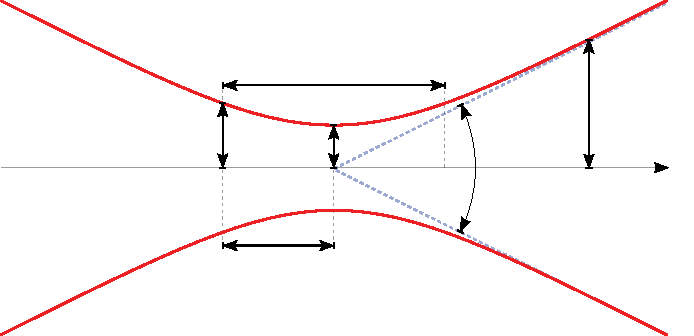
\includegraphics[width=\unitlength]{results_and_discussion/assets/GaussianBeamWaist_wiki.pdf}}%
    \put(0.20711366,0.258742){\color[rgb]{0,0,0}\makebox(0,0)[lb]{\smash{$\sqrt{2}\omega_0$}}}%
    \put(0.46945764,0.3786023){\color[rgb]{0,0,0}\makebox(0,0)[lb]{\smash{$b$}}}%
    \put(0.40642304,0.25814167){\color[rgb]{0,0,0}\makebox(0,0)[lb]{\smash{$\omega_0$}}}%
    \put(0.88008299,0.33378319){\color[rgb]{0,0,0}\makebox(0,0)[lb]{\smash{$\omega(z)$}}}%
    \put(0.97412911,0.23552655){\color[rgb]{0,0,0}\makebox(0,0)[lb]{\smash{$z$}}}%
    \put(0.7029858,0.28052652){\color[rgb]{0,0,0}\makebox(0,0)[lb]{\smash{$\vartheta$}}}%
    \put(0.38180954,0.10125008){\color[rgb]{0,0,0}\makebox(0,0)[lb]{\smash{$z_\mathrm{R}$}}}%
  \end{picture}%
\endgroup%

	\caption{The geometry of a focal region of a laser beam. The beam is
	considered to be cylindrically symmetric about the $z$ axis, the effective
	volume of the Raman sample was taken to be the volume of a cylinder of
	diameter $2\omega_0$ and length $2b$. Adopted from
	\textcite{GaussianBeamWaist}.}
	\label{\figlabel{GaussianBeamWaist_wiki}}
\end{figure}

The beam radius $\omega(z)$ can be described as the function of $z$
coordinate by equation
\begin{equation}
	\omega(z) = \omega_0\sqrt{1+\left(\frac{2z}{b}\right)^2}.
	\label{\eqnlabel{focus_optimization:beam_radius}}
\end{equation}

As a first estimation, consider non-resonance Raman scattering produced from
homogenous infinite medium and arising only from the region with the highest
illumination intensity. Furthermore, assume the loss of the illumination beam
intensity due to the Raman scattered light as negligible and that the Raman
medium is fully transparent to excitation and scattered light, it means that
there is negligible absorption and stimulated emission. The amount of Raman
scattered light from the thin transverse slice of the excitation beam is
independent of the distribution of the energy in the slice and therefore is
proportional to the total illuminating laser-beam power under these
assumptions. Then, view the Raman emission from the particular direction in
the plane of the slice. The emitted flux would be the integrated flux from
all elements on the line intersecting the slice so there would be a linear
increase of the number of elements with the increasing diameter, but each
element illumination power decreases with the square of the diameter of the
illuminating beam.

Considering the \eqnref{focus_optimization:beam_radius} derive the
approximate dependence of irradiance of that point by the Raman-scattered
light on the $z$ coordinate
\begin{equation*}
	I \propto \frac{1}{\omega(z)} \propto \frac{1}{\sqrt{1 + (2z/b)^2}}.
	\label{\eqnlabel{focus_optimization:slice_irradiance}}
\end{equation*}

So, the irradiance at $z = b$ will be reduced from the $z = 0$ by a factor of
$1/\sqrt{5} \doteq 0.447 \doteq 1/2$. For the next calculation, the brightest
region of excitation beam was approximated by the “source cylinder” of length
$2b$ and diameter $2\omega_0$ and therefore included only the brightest
region of Raman emission and neglect the emission from less-bright regions.
The source parameters are then \parencite{Barrett1968}:
\begin{align}
	\text{length:}&
		& L_\text{E}& = 16\lambda/(\text{\g{p}}\vartheta^2)
	\label{\eqnlabel{focus_optimization:L_E}}\\
	\text{diameter (width of scattering area):}&
		& W_\text{E}& = 4\lambda/(\text{\g{p}}\vartheta)
	\label{\eqnlabel{focus_optimization:W_E}}\\
	\text{volume:}&
		& V_\text{E}& = 64 \lambda^3/(\text{\g{p}}^2\vartheta^4)
	\label{\eqnlabel{focus_optimization:V_E}}\\
	\text{length-to-diameter ratio:}&
		& L_\text{E}/W_\text{E}& = 4/\vartheta.
	\label{\eqnlabel{focus_optimization:LW_E}}
\end{align}

These approximations apply to diffraction-limited Gaussian beams (
TEM\textsubscript{00}), for low-order transverse modes or combination of such
modes, the calculations based on these equations can be considered accurate
within an order of magnitude.

Many simple arguments \parencite{Atwood1963,Barrett1968} were used to propose
that the Raman spectrometer using right angle geometry scattering geometry
will gain higher signal if the laser beam is more focused. None of these
arguments, however, do not establish if there is an optimum degree of
focusing less then the largest practical value. \textcite{Barrett1968} showed
that such an optimum exists theoretically; they calculated its approximate
value, and they compared the Raman power that can be usefully collected at
that optimum degree of focusing with the total emitted Raman power.

It is known that the light is scattered to all directions by the Raman effect
and within the assumptions stated above, the Raman intensity is linearly
proportional to the excitation laser beam power. Therefore, if the amount of
Raman scattered light gathered by the spectrometer should be maximized, the
light needs to be collected from the largest solid angle and the largest
possible illuminated volume. Typical Raman spectrometer light collecting path
has two optical parts, spectrograph, and light collecting optics. Let
consider their parameters as given even though similar considerations as
bellow can also be applied to the light collecting optics optimization. Lets
further consider that the spectrograph consists of an entrance slit, imaging
optics, dispersing element, and CCD camera.

For simplicity approximate the source as flat ribbon with the same length and
width as specified above for the “source cylinder” which radiates uniformly
to all collected angles from all parts of its surface. Then, consider that
the light collecting optic displays the entrance slit of the spectrograph to
the center of the focal region of the illuminating beam. The width of the
slit $W_\mathrm{s}$ is determined by the spectrograph settings, particularly
by the desired spectral resolution, and its length $L_\mathrm{s}$ could be
estimated as an image of the CCD chip through the spectrograph. Moreover,
suppose that the aperture of light collecting optic is large enough further
not to constrain the collected Raman light over the spectrograph aperture.

Then there are two competing processes. The assumptions above that the amount
of the Raman scattered light from all thin transverse slices of the
excitation beam is the same implies that the total amount of Raman scattered
light from the source ribbon is dependent only on its length. As the focal
length of the excitation beam focusing lens is decreased, the source ribbon
is getting narrower, which results in more intensive emission of the
scattered light per unit area. So if we start with the source ribbon width
larger than the image of the spectrograph entrance slit width, the amount of
collected light increases with the narrower source ribbon. In the opposite,
the length (and therefore the total Raman scattered light intensity) of the
source ribbon decreases with the decreasing focal length of the excitation
beam focusing lens and so when the source ribbon gets shorter than the image
of the spectrograph entrance slit length, the amount of collected light
decreases with the shorter source ribbon.

So, lets split further analysis of the dependence of the Raman flux
transmitted through the spectrometer on the focusing angle of the excitation
beam $\vartheta$ (\eqnref{focus_optimization:theta}) to regions divided by
two focusing angles $\vartheta_\mathrm{W}$ and $\vartheta_\mathrm{L}$. The
$\vartheta_\mathrm{W}$ defines focusing angle at which the width of the
focusing ribbon $W_\text{E}$ is the same as the width $W$ of image of the
spectrograph entrance slit width $W_\text{S}$, and $\vartheta_\mathrm{L}$ is
angle which causes equality of the source ribbon length $L_\text{E}$ and
length $L$ of the spectrograph entrance slit image length $L_\text{S}$ on the
source. Further, define magnification of the scattered light collecting
optics as $M$. Then
\begin{align}
	L& = \frac{L_\mathrm{S}}{M}
	\label{\eqnlabel{focus_optimization:slit_length_magnification}}\\
	W& = \frac{W_\mathrm{S}}{M}
	\label{\eqnlabel{focus_optimization:slit_width_magnification}}
\end{align}
and using \eqnref{focus_optimization:L_E} and
\labelcref{\eqnlabel{focus_optimization:W_E}} and putting $L = L_\mathrm{E}$
and $W = W_\mathrm{E}$ respectively we get
\begin{align}
	\vartheta_\mathrm{W} = \frac{4\lambda}{\text{\g{p}}W}
		= \frac{4\lambda M}{\text{\g{p}}W_\mathrm{S}}
	\label{\eqnlabel{focus_optimization:theta_W}}\\
	\vartheta_\mathrm{L} = \sqrt{\frac{16\lambda}{\text{\g{p}}L}}
		= \sqrt{\frac{16\lambda M}{\text{\g{p}}L_\mathrm{S}}}.
	\label{\eqnlabel{focus_optimization:theta_L}}
\end{align}

For our spectrometer, we have $W_\mathrm{S} = 50$\,\g{m}m and beam diameter
$d = 0.9$\,mm. The wavelength can be calculated from the wavelength in vacuum
$\lambda_0 = 257.2$\,nm divided by the refractive index of water
$n_{257} = 1.3598$ \parencite{Hale1973} $\lambda = 189.1$\,nm The
$L_\mathrm{S}$ can be calculated from the height of the CCD chip
$L_\text{CCD} = 6.9$\,mm and magnification of spectrograph
$M_\text{spc} = 1.1$ as
$L_\text{S} = L_\text{CCD}/M_\text{spc} \doteq 6.3$\,mm, the magnification $M$
may be computed from focal length of objective $f_\text{o} = 13$\,mm and
focusing lens before monochromator $f \text{c} = 101.6$\,mm as
$M = f_\text{c}/f_\text{o} \doteq 7.82$. Then, from the above equations, we
calculate
\begin{align}
	\vartheta_\mathrm{W} \doteq 0.0376
	\label{\eqnlabel{focus_optimization:theta_W_calc}}\\
	\vartheta_\mathrm{L} \doteq 0.0346,
	\label{\eqnlabel{focus_optimization:theta_L_calc}}
\end{align}
which correspond regarding \eqnref{focus_optimization:theta} to
\begin{align}
	f_\mathrm{W} \doteq 24\,\text{mm}
	\label{\eqnlabel{focus_optimization:f_W_calc}}\\
	f_\mathrm{L} \doteq 26\,\text{mm}
	\label{\eqnlabel{focus_optimization:f_L_calc}}
\end{align}
respectively.

We can note, that $\vartheta_\mathrm{W}$ is greater then
$\vartheta_\mathrm{L}$, which is according to \textcite{Barrett1968} common
for the tabletop spectrometer with moderate resolution and with fairly fast
focal ration. So we can divide further analysis into three regions according
to excitation beam focusing angle
$\vartheta$: $0 \leq \vartheta < \vartheta_\text{L}$;
$\vartheta_\text{L} < \vartheta < \vartheta_\text{W}$;
$\vartheta_\text{W} < \vartheta$.

Under the approximations above the Raman flux fraction $F$, collected by the
spectrometer of the total Raman flux emitted by the source ribbon into all
angles (i.e. full solid angle of $4\text{\g{p}}$), can be estimated now. For
the simplicity, polarization effects of input and output are further ignored
and the Raman emission is assumed isotropic over all angles of collection.
Define the solid angle subtended by the spectrometer pupil as
$\Omega_\mathrm{S}$ and corresponding scattered light collecting solid angle
at the source ribbon as $\Omega$. Then
\begin{equation}
	\Omega = \Omega_\mathrm{S}M^2.
	\label{\eqnlabel{focus_optimization:omega_magnification}}
\end{equation}
For our spectrometer the solid angle of acceptance of monochromator may be
calculated from monochromator $f/\# = f/6.4$ as
$\Omega_\text{S} =
	2\text{\g{p}}\left[1 - \cos\left(\arctan\frac{1}{6.4}\right)\right]
	\doteq 0.075$\,rad.

The Raman flux fraction $F$ is then calculated from the solid angle fraction
$\Omega / 4\text{\g{p}}$ and the fraction of the light which is “masked out”
by the width of the slit image and fraction of the ribbon length as compared
to the height of the slit image using \cref{%
\eqnlabel{focus_optimization:L_E},%
\eqnlabel{focus_optimization:W_E},%
\eqnlabel{focus_optimization:slit_length_magnification},%
\eqnlabel{focus_optimization:slit_width_magnification},%
\eqnlabel{focus_optimization:omega_magnification}}.

For the first $0 \leq \vartheta < \vartheta_\text{L}$ region, the whole

slit-image width and height are illuminated, but the focused beam is wider
than slit width, and therefore the radiant flux density in the sample is
smaller (recall that we assumed that radiant losses in the sample are
negligible)
\begin{equation}
	F_\text{I}(\vartheta)
		= \frac{W}{W_\text{E}}\cdot\frac{\Omega}{4\text{\g{p}}}
		= \frac{\frac{W_\text{S}}{M}}{\frac{4\lambda}{\text{\g{p}}\vartheta}}
			\cdot\frac{\Omega_\text{S}M^2}{4\text{\g{p}}}
		=	\frac{W_\text{S}\Omega_\text{S}M}{16\lambda}\vartheta.
	\label{\eqnlabel{focus_optimization:F_I}}
\end{equation}

In the next second region
$\vartheta_\text{L} < \vartheta < \vartheta_\text{W}$,
only the whole slit-image width is illuminated, but the exciting beam is
focused to an area with smaller length than is the slit length and so the
radiant flux density is diminished by the ratio between scattering area
length and slit-image length
\begin{equation}
	F_\text{II}(\vartheta)
		= \frac{W}{W_\text{E}}\cdot\frac{\Omega}{4\text{\g{p}}}
			\cdot\frac{L_\text{E}}{L}
		=	\frac{\frac{W_\text{S}}{M}}{\frac{4\lambda}{\text{\g{p}}\vartheta}}
			\cdot\frac{\Omega_\text{S}M^2}{4\text{\g{p}}}
			\cdot\frac{\frac{16\lambda}{\text{\g{p}}\vartheta^2}}
				{\frac{L_\text{S}}{M}}
		= \frac{W_\text{S}\Omega_\text{S}M^2}{\text{\g{p}}L_\text{S}}
			\cdot\frac{1}{\vartheta}.
	\label{\eqnlabel{focus_optimization:F_II}}
\end{equation}

The Raman scattering area in the third region $\vartheta_\text{L} < \vartheta$
is so small that the Raman scattered light is collected from the whole beam,
and therefore whole radiant flux is used
\begin{equation}
	F_\text{III}(\vartheta)
		= \frac{\Omega}{4\text{\g{p}}}\cdot\frac{L_\text{E}}{L}
		= \frac{\Omega_\text{S}M^2}{4\text{\g{p}}}
			\cdot\frac{\frac{16\lambda}{\text{\g{p}}\vartheta^2}}
				{\frac{L_\text{S}}{M}}
		= \frac{4\lambda\Omega_\text{S}M^3}{\text{\g{p}}^2L_\text{S}}
			\cdot\frac{1}{\vartheta^2}.
	\label{\eqnlabel{focus_optimization:F_III}}
\end{equation}

\begin{figure}
	\centering
	\input{results_and_discussion/assets/F}
	\caption{A plot of the values of the fractional Raman flux $F$ as calculated
	for our experimental conditions using \cref{%
		\eqnlabel{focus_optimization:F_I},\eqnlabel{focus_optimization:F_II},%
		\eqnlabel{focus_optimization:F_III}}
	versus the focusing angle $\vartheta$ of the
	illuminating laser beam.}
	\label{\figlabel{focus_optimization:F}}
\end{figure}

The results of \cref{%
		\eqnlabel{focus_optimization:F_I},%
		\eqnlabel{focus_optimization:F_II},%
		\eqnlabel{focus_optimization:F_III}}

for our experimental setup can be seen in \figref{focus_optimization:F}. The
optimum value of $\vartheta$ is $\vartheta_\text{L}$. \textcite{Barrett1968}
proposed the optimum value to lie above the $\vartheta_\text{L}$ because the
signal from outside the cylinder along the excitation beam axis is also
transmitted through the spectrometer in the second and third region, but they
do not expect the optimum as high as $\vartheta_\text{W}$. The light
collecting optics magnification can be optimized according to the equations
from above too, but each equation must be multiplied by the length of the
slit image $L$. The Raman signal then does not decrease with the
magnification, which means that the magnification should be used as high as
practical.

From these considerations follows conclusion for our experimental setup, that
the optimal focal length of the laser beam focusing lens for the off-
resonance Raman spectroscopy should be somewhere between 18 and 22\,mm which
is impractically small.

All the above calculations, however, neglected loss of the excitation beam
power as it goes through the sample, but we want to use the instrument for
resonance Raman spectroscopy where significant absorption inside the sample
occurs. It can decrease the length of the source cylinder $L_E$ significantly
and can push the $\vartheta_\text{L}$ to much lower values. For example, we
typically use samples with absorbance between 5 and 50 at 257\,nm in a 1cm
cuvette. So, for example, the intensity of incident light is halved in
300\,\g{m}m path through the sample with absorbance 10 but the
$L_E = 802$\,\g{m}m at $\vartheta_\text{L}$. If we correct the
\eqnref{focus_optimization:L_E} to for example one fourth, then the
corrected $L_E,corr$ would be approximately 170\,\g{m}m and corresponding
focal length of the laser beam focusing lens about 52\,mm.

The absorbing medium brings additional complications. For example, the
anomalous refractive index near the absorption band can significantly
influence the focused beam waist, and laser beam absorption can cause local
heating which also influences refractive index and moreover produces currents
in the sample. There is also a dependence of the optimal focal length on the
excitation wavelength, but exchanges of the focusing lens in dependence on
the excitation wavelength was impractical.

However, in conclusion, the focusing lens should have the focal length as
small as possible following the experimental geometric constraints.

\subsection{Wavenumber calibration}
\label{wavenumber_calibration}

For correct Raman spectra interpretation we needed precise wavenumber
calibration. It can be done by measuring spectrum with known line positions
in the same spectrometer configuration as for the spectrum of the sample and
then interpolating and extrapolating the wavenumbers from these known line
positions to all detector pixels. One group of calibration spectra are Raman
spectra of organic solvents but you can't use pure indene which is widely
used in visible Raman because it strongly absorbs in UV and its lines can be
shifted if you dilute it. So other solvents need to be found. Organic
solvents were used as wavenumber calibration for first UV Raman spectra
measurements, for example \textcite{Harada1975} calibrated to Raman line of
\ch{CCl4}. But early, it was clear, that single organic solvent is not
satisfactory and therefore some teams started to use mixtures of solvents.
If you use mixture of solvents, you don't know, how the components influece
each other, they can evaporate in different rate so their ratio can be
changing which can shift their bands. You can solve this problem by measuring
the solvents separately but then you prolong the time spend for calibration
spectra measurement. Some selected solvents are listed in
\tabref{wavenumber_calibration:solvents}.

\begin{table}
	\centering
	\begin{tabular}{m{8.7cm}l}
\toprule
solvent & citation \\
\midrule
\ch{CCl4}                                   & \textcite{Harada1975} \\
\addlinespace[.3em]
cyclohexane                                 & \textcite{Myers1988} \\
\addlinespace[.3em]
acetonitrile                                & \textcite{Gustafson1988} \\
\addlinespace[.3em]
ethanol                                     & \textcite{Su1990} \\
\addlinespace[.3em]
ethyl acetate/dioxane (2:1 v/v)             & \textcite{Toyama1991} \\
\addlinespace[.3em]
cyclohexane, acetone                        & \textcite{Kaminaka1992} \\
\addlinespace[.3em]
acetonitrile, acetone                       & \textcite{Benson1992} \\
\addlinespace[.3em]
cyclohexanone/acetonitrile (1:1 v/v)        & \textcite{Hashimoto1993} \\
\addlinespace[.3em]
ethanol, \textit{n}-penthane                & \textcite{Mukerji1995} \\
\addlinespace[.3em]
dioxane, \ch{CCl4}, acetonitrile            & \textcite{Russell1995} \\
\addlinespace[.3em]
ethyl acetate/dioxane (2:1 v/v) (257\,nm)
                                            & \textcite{Fujimoto1998} \\
\addlinespace[.3em]
cyclohexanone/acetonitrile (1:1 v/v) (213\,nm)
                                            & \textcite{Fujimoto1998} \\
\addlinespace[.3em]
acetone, ethanol, pentane                   & \textcite{Mukerji1998} \\
\addlinespace[.3em]
\textit{n}-pentane, cyclehexane, dimethylformamide, ethanol, acetonitrile,
acetic acid                                 & \textcite{Billinghurst2006} \\
\addlinespace[.3em]
dimethylsulfoxide                           & \textcite{Srivastava2008} \\
\addlinespace[.3em]
dimethyl formamide, acetonitrile, trichloroethylene, isopropanol, indene,
cyclohexane                                 & \textcite{Jayanth2009} \\
\addlinespace[.3em]
cyclohexane, \textit{N,N}-dimethylformamide, methanol, acetonitrile,
dimethyl sylfoxide, acetic acid             & \textcite{Oladepo2011} \\
\addlinespace[.3em]
acetonitrile, isopropanol, cyclohexane and dimethyl formamide
                                            & \textcite{Mondal2016} \\
\bottomrule
\end{tabular}

	\caption{%
		Selection of organic solvents which were used for UV Raman spectra
		wavenumber calibration in literature.%
	}
	\label{\tablabel{wavenumber_calibration:solvents}}
\end{table}

Some laboratories were not satisfied with the separate calibration and used
also internal standard to improve the calibration of spectra. For example,
\textcite{Wen1998} used \ch{Na2SO4} as internal frequency (981\,\icm) standard,
and Raman frequencies were calibrated to $\pm1 $\,\icm{} using
\ch{ccl4}/\ch{CH3CN} mixture.

The other approach was also to use the elastically scattered laser line.
 \textcite{Kumamoto2012} calibrated grating dispersion with the laser line
(0\,\icm), and Raman bands of boron nitride (1370\,\icm) and acetonitrile
(2249\,\icm).

%\textcite{Myers1988} calibrated wavenumbers using cyclohexane in
combination with various \ch{H2} Raman-shifted laser lines and mercury
emission lines. \textcite{Su1990} calibrated Raman spectra in frequency with
ethanol. \textcite{Toyama1991, Toyama1996} used for wavenumber calibration
the Raman bands of ethyl acetate/dioxane (2:1 v/v), which had been measured
with visible-laser excitation on a spectrometer calibrated with indene Raman
bands and neon emission lines. \textcite{Kaminaka1992} calibrated Raman
shifts with cyclohexane and acetone as the secondary standard, while their
Raman bands were calibrated with indene, with the use of visible excitation.
\textcite{Benson1992} calibrated the wavenumber shift with the use of the
Raman spectra of acetonitrile and acetone. \textcite{Benson1993} used carbon
tetrachloride for wavenumber shift calibration standard.
\textcite{Hashimoto1993} made wavenumber calibration with the Raman bands of
cyclohexanone/acetonitrile (1:1 v/v). \textcite{Mukerji1995} calibrated spectra
against neat solution of ethanol and \textit{n}-penthane.
\textcite{Russell1995} performed wavenumber calibration in UV-laser excited
Raman spectra using the well known Raman lines of dioxane, carbon
tetrachloride, and acetonitrile. \textcite{Gustafson1988} calibrated
wavenumber shift using the Raman spectrum of acetonitrile.
\textcite{Leonard1994} calibrated wavenumber shift with the use of the Raman
spectrum of cyclohexane. \textcite{Takeuchi1990} made wavenumber calibration
by using the Raman bands of cyclohexanone/acetonitrile (1:1, v/v), the
wavenumber of which had been established with visible-laser excitation on a
spectrometer calibrated with indene Raman bands and neon emission lines.
\textcite{Takeuchi1995} calibrated wavenumber axis of the spectra by using
the spectrum of a mixture solution of ethyl acetate/dioxane (2:1 v/v) as a
wavenumber standard. \textcite{Tuma1995} performed wavenumber
calibration in UVRR spectra using well-known Raman lines of dioxane, carbon
tetrachloride, and acetonitrile. \textcite{Wen1997} calibrated Raman
frequencies using a standard liquid mixture of carbon tetrachloride and
acetonitrile. \textcite{Fujimoto1998} made wavenumber calibration of the
spectra by use of the Raman bands of a 2:1 (v/v) mixture of ethyl
acetate/1,4-dioxane (257\,nm excitation) or of a 1:1 (v/v) mixture of
cyclohexanone/acetonitrile (213\,nm). \textcite{Mukerji1998} calibrated data
with acetone, ethanol, and pentane. \textcite{Wen1998} used \ch{Na2SO4} as
internal frequency (981\,\icm) standard, and Raman frequencies were
calibrated to $\pm1 $\,\icm{} using \ch{ccl4}/\ch{CH3CN} mixture.
\textcite{Suen1999} calibrated against neat solutions of ethanol and acetone,
for which the Raman band frequencies were known. \textcite{Toyama1999}
performed wavenumber calibraion by use of the Raman bands of
ethylacetate--dioxane (2:1, v/v). \textcite{Wen1999} calibrated Raman
frequencies by using a standarad liquid mixture of carbon tetrachloride and
acetonitrile. \textcite{Sokolov2000} calibrated data with acetone, ethanol and
pentane. \textcite{Toyama2001} made wavenumber calibration of Raman spectra
by using the Raman spectrum of a 2:1 (v/v) mixture of ethylacetate/1,4-dioxane.
\textcite{Fujimoto2002} calibrated Raman spectrometer by using the Raman bands
of a 2:1 (v/v) mixture of ethylacetate and dioxane for 257-nm excitation or a
1:1 (v/v) mixture of cyclohexanone and acetonitrile for 229-nm excitation.
\textcite{Toyama2002} performed wavenumber calibration of Raman spectra by use
of the Raman bands of a 2:1 (v/v) mixture of ethyl acetate and 1,4-dioxane.
\textcite{Nelson2004} calibrated the Raman shift axis with pure ethanol.
\textcite{Toyama2005,Toyama2005a} made wavenumber calibration of Raman spectra
by use of Raman bands of a 2:1 (v/v) mixture of ethyl acetate and 1,4-dioxane.
\textcite{Billinghurst2006,Billinghurst2006a} perforemd frequency calibration
by measuring the Raman scattering of organic solvents for whom the peak
positions are known (\textit{n}-pentane, cyclehexane, dimethylformamide,
ethanol, acetonitrile, and acetic acid). \textcite{Jirasek2006} wavenumber
calibrated abscissa of each acquired spectrum using an ethanol spectrum as the
calibration standard. \textcite{Kundu2007} performed frequency calibration by
measuring the resonance Raman spectra of organic solvents whose peak positions
were known (acetonitrile, dimethylformamide, \textit{n}-hexane,
\textit{n}-pentane, cyclohexane and acetic acid). \textcite{Yarasi2007}
performed frequency calibration by measuring Raman scattering of solvents of
known frequencies (acetonitrile, dimethylformamide, carbon tetrachloride,
ethanol, and pentane). \textcite{Knee2008} calibrated spectra against ethanol,
acetone and pentane. \textcite{Billinghurst2009} performed calibration by
measuring the Raman scattering of solvents for which the peak positions are
known (\textit{n}-pentane, cyclohexane, \textit{N,N}-dimethilformamide,
ethanol, acetonitrile, and acetic acid). \textcite{Jayanth2009} calibrated
spectra using known solvent bands (dimethyl formamide, acetonitrile,
trichloroethylene, isopropanol, indene, and cyclohexane). \textcite{Shaw2009}
used a spectrum of ethanol to calibrate the abscissa of each spectrum.
\textcite{Jayanth2011} carried out calibration using spectra of standard
solvents: dimethyl formamide, acetonitrile, trichloroethylene, isopropanol,
indene, and cyclohexane. \textcite{Oladepo2011} performed frequency calibration
by measuring the Raman scattering of solvents for which the peak positions were
known (cyclohexane, \textit{N,N}-dimethylformamide, methanol, acetonitrile,
dimethyl sylfoxide and acetic acid). \textcite{Billinghurst2012} performed
frequency calibration by measuring the Raman scattering of organic solvents for
which the peak positions are known (\textit{n}-pentane, cyclohexane,
dimethylformamide, ethanol, acetonitrile and acetic acid).
\textcite{Kumamoto2012} calibrated grating dispersion with the laser line
(0\,\icm), and Raman bands of boron nitride (1370\,\icm) and acetonitrile
(2249\,\icm). \textcite{Srivastava2008,Muntean2013} used Raman spectra of
dimethylsulfoxide as a standard for wavenumber calibration.
\textcite{Mondal2016} calibrated the recorded spectra using known bands of
standard solvents, e.g. acetonitrile, isopropanol, cyclohexane and dimethyl
formamide.


Calibration to the Raman spectrum of organic solvent has an advantage that
you don't need to know the exact wavelength of excitation beam typically to
precision in the order of $10^{-3}$\,nm. The wavelength of the source also
does not need to be stable to this precision between measurements. You can
also measure the calibration spectrum from the same place and in the same
configuration as the sample so there is no danger of some offsets caused by
changes in the geometrical alignment of spectrometer, for example when you
move with objective during focusing the light gathering part of the
spectrometer on the sample or change filters in the gathered light path. The
big disadvantage of calibration to the Raman spectra of organic solvents is
that their Raman bands are broad and overlapping and therefore their
positions can't be determined with sufficiently high precision. We can
achieve precision of $\pm1$ \,\icm{} for well-resolved dominant and a few
\icm{} for shoulders or weak bands. Organic solvents also do not usually have
much bands in the region between 1800 and 2800\,\icm{} and don't have
sufficiently large number of usable Raman lines especially if you want
solvents which are usable in deep UV.

We had good experience with the other approach to calibration which uses
atomic emission spectra of some standard lamp. Usually, as it is also the
case in our laboraty, the neon lamp is used. But this lamp do not cover deep
UV range of light so we decided to try some organic solvents for UV Raman
calibration as they were broadly used as you can see from the
\tabref{wavenumber_calibration:solvents}.

We selected cyclohexane because it has pretty rich Raman spectrum. We also
wanted to solve the problem, that most of the standard organic solvents
does not have much bands in the region between 1800 and 2800\,\icm{} so we
decided that we also use deuterated cyclohexane-d12 which nicely fills that
region. To our knowledge, the cyclohexane-d12 was not used for calibration of
UV Raman spectra of nucleic acids before.

The spectra of cyclohexane and cyclohexane-d12 was measured on home-made Raman
spectrometer using visible excitation of 532\,nm \REFERENCE{}
\textcolor{red}{(description should be in materials and methods)}
and calibrated to the spectrum of neon calibration lamp. At least 3 and
typically 8 spectra for each Raman line with different grating position were
taken. The top half of the well resolved peaks was fitted to gaussian
curve and its precise postion was estimated. All the measured positions were
then averaged. The results can be seen in
\tabref{wavenumber_calibration:cyclohexane_wavenumbers}.

\begin{table}
	\centering
	\begin{tabular}{lr@{\,$\pm$\,}lr@{.}l}
\toprule
\multicolumn{1}{c}{name} & \multicolumn{2}{c}{$\bar{\nu}$ (\icm)}
	& \multicolumn{2}{c}{x (px)} \\
\midrule

D1   &  298.55 & 0.08 & 2002&68 \\
D2   &  373.77 & 0.06 & 1952&43 \\
H1   &  384.19 & 0.15 & 1943&28 \\
H2   &  426.75 & 0.13 & 1914&58 \\
D3a  &  636.15 & 0.09 & 1775&71 \\
D3   &  724.48 & 0.10 & 1715&56 \\
D5   &  795.93 & 0.09 & 1666&70 \\
H3   &  802.41 & 0.13 & 1660&07 \\
D6   &  939.10 & 0.12 & 1568&22 \\
D7   & 1014.07 & 0.12 & 1516&56 \\
H5   & 1028.91 & 0.14 & 1503&78 \\
D8   & 1073.70 & 0.11 & 1474&89 \\
D9   & 1120.05 & 0.10 & 1442&68 \\
H6   & 1158.77 & 0.13 & 1413&54 \\
D10  & 1214.12 & 0.08 & 1376&89 \\
H7   & 1267.25 & 0.11 & 1337&14 \\
H8   & 1444.81 & 0.11 & 1211&48 \\
D11  & 1706.70 & 0.04 & 1026&44 \\
H13  & 1720.30 & 0.06 & 1014&25 \\
D12  & 1753.42 & 0.04 &  992&68 \\
H13a & 1765.45 & 0.03 &  981&85 \\
D16  & 1979.06 & 0.06 &  828&31 \\
D17  & 2004.03 & 0.06 &  810&09 \\
H14  & 2052.09 & 0.03 &  772&50 \\
D18  & 2083.28 & 0.05 &  751&69 \\
D19  & 2106.41 & 0.06 &  734&77 \\
H14a & 2117.79 & 0.05 &  723&54 \\
D21  & 2154.45 & 0.05 &  699&13 \\
D23  & 2198.41 & 0.05 &  666&48 \\
D25  & 2322.52 & 0.04 &  574&26 \\
H15  & 2350.57 & 0.03 &  550&63 \\
H16  & 2634.46 & 0.03 &  336&50 \\
H20  & 2853.91 & 0.05 &  168&13 \\
D28  & 2885.28 & 0.05 &  146&18 \\
D29  & 2914.56 & 0.06 &  123&83 \\
H21  & 2924.74 & 0.04 &  113&34 \\
H22  & 2939.47 & 0.05 &  102&30 \\

\bottomrule
\end{tabular}

	\caption{%
		Estimated wavenumbers $\tilde{\nu}$ of cyclohexane (H) and cyclohexane-d12
		(D) with the corresponding pixel positions $x$ from UV Raman measurement.%
	}
	\label{\tablabel{wavenumber_calibration:cyclohexane_wavenumbers}}
\end{table}

Spectrum of cyclohexane and cyclohexane-d12 can be then measured after each
UV Raman measurement in such a way, that measured sample is replaced by
calibration sample so that the calibration samples are measured from the same
place as the measured sample (with the same grating position of spectrograph).
The precise pixel positions of their Raman lines was estimated from the
spectrum in the same way as in the visible Raman measurements. These pixel
positions can be then matched to known approximate pixel positions of
cyclohexane and cyclohexane-d12 using appropriate weight function which
favors matches with more bands then less by moving the measured spectrum along
the table with calibration spectrum with for example 0.5-px step. The outcome
of this step is calibration lines wavenumbers in dependence on their pixel
positions. They can be fitted by 3rd degree polynomial to assign the
wavenumbers to all the 2048 detector pixels. The spectrum is then linearly
interpolated to have 1-\icm{} steps. Example UV Raman spectra of cyclohexane
and cyclohexane-d12 calibrated by our home-made calibration program with
highlighted band positions can be seen in
\figref{wavenumber_calibration:cyclohexane_spc}.

\begin{figure}
	\centering
	\input{results_and_discussion/assets/cyclohexane_calibration/%
cyclohexane_calibration}
	\caption{%
		UV Raman spectrum of cyclohexane and cyclohexane-d12 with 244-nm
		excitation. Grey lines denotes the positions of Raman lines used for
		calibratin (see
		\tabref{wavenumber_calibration:cyclohexane_wavenumbers}).%
	}
	\label{\figlabel{wavenumber_calibration:cyclohexane_spc}}
\end{figure}

As was written above, for sub-\icm{} calibration precision, the different
method then calibration to organic solvents needs to be used. Some authors
proposed calibration to atomic lines of mercury lamp, for example
\textcite{Manoharan1990,Efremov1991} calibrated the spectrograph with the
253.6-, 312.6-, and 365-nm lines of a low-pressure Hg lamp. The disadvantage
of usage of low pressure Hg-lamp is that its lines are rather sparse so
other approaches, which combined the Hg spectrum with other methods were
proposed. For example, \textcite{Myers1988} calibrated wavenumbers using
cyclohexane in combination with various \ch{H2} Raman-shifted laser lines and
mercury emission lines.

We tried to use mercury lamp too but it didn't bring any new precision to the
calibrated spectra so we tried to search for the different calibration source.
There was similar effort in \textcite{Wert2014}, who proposed calibration with
zinc (202.5, 206.2, and 213.9\,nm) and cadmium (214.4, 226.5, and 228.8\,nm)
standard lamps and Positive Light Indigo-S 210 -- 240\,nm tunable Ti:Sa laser
if necessary. But we pursued different approach and took inspiration from
calibration of space instruments which broadly use hollow cathode platinum
lamp \parencite{Mount1977,Reader1990,Sansonetti1992} for calibration in UV
spectral range.

\emph{Hollow cathode lamps} (HCL) are routinely used in \emph{atomic absorption
spectroscopy} (AAS) and therefore they are commercially available on the market
together with power supplies because HCL requires precision current source. We
used P209 HCL Power Supply (Photron) with P840 Hollow Cathode Lamp -- Pt
(Photron) which provided stable platinum atomic spectrum right after start. The
new spectrometer schema with calibration source is in
\figref{wavenumber_calibration:apparatus_schema}.
The callibration beam was guided by right-angle prisms in total internal
reflection mode (MC1 and MC2). We chose prisms instead of mirrors because they
are much more stable in time and we don't need to have any concerns about their
aging. Prism MC2 was placed on motorized flip mount so we can easily switch
between measurement of calibration spectra and Raman spectra from samples.
The calibration beam was colimated by the lens LC1 with focal length of
10\,cm (Thorlabs) and could be attenuated by the aperture AC1 which was
represented by iris diaphragm (Thorlabs).

\begin{figure}
	\centering
	\begin{tikzpicture}[font=\sffamily]

% settings
\newcommand*{\cellBorderWidth}{3\pgflinewidth}
\newcommand*{\cellLineWidth}{1.5\pgflinewidth}
\definecolor{glassBorderColor}{RGB}{0,128,255}
\definecolor{glassFillColor}{RGB}{230,242,255}
\definecolor{waterFillColor}{RGB}{0,128,255}
\definecolor{hclColor}{RGB}{255,128,0}
\tikzset{
	clip
}
\tikzset{
	mirror element/.style={color=black, line width=2*\pgflinewidth},
	real laser beam/.style={color=cyan, line width=2*\pgflinewidth},
	laser beam/.style={color = black, opacity = 0.2,%
		line width = 2*\pgflinewidth},
	scattered ray/.style={color = black, opacity = 0.2,%
		line width = 1.5*\pgflinewidth},
	scattered fill/.style={fill=black, draw=none, fill opacity=0.1},
	glass/.style={color=glassBorderColor, opacity=0.5,%
		fill=glassFillColor, fill opacity=0.5},
	sample cell/.style={color=glassBorderColor, opacity=0.5,%
		double=glassFillColor, double distance=\cellBorderWidth,
		line width=\cellLineWidth, line cap=rect},
	water fill/.style={fill=waterFillColor, fill opacity=0.1},
	mirror surface/.style={color=black!20, fill=black!10},
	nd filter/.style={color=black, opacity=0.2, fill=black, fill opacity=0.1},
	nd carousel/.style={color=black, opacity=0.4, fill=black, fill opacity=0.2},
	notch/.style={color=black, opacity=0.4, fill=black, fill opacity=0.1},
	aperture/.style={color=black, line width=2*\pgflinewidth},
	aperture filldraw/.style={color=black!40, fill=black!20, clip even odd rule},
	clip even odd rule/.code={\pgfseteorule},
	shutter/.style={nd carousel},
	shutter blade/.style={solid, line width = 1.5*\pgflinewidth, opacity = 0.4},
	hcl/.style={nd carousel},
	hcl lamp/.style = {color = hclColor, line width = 3 * \pgflinewidth,%
		line cap = round},
	hcl ray/.style = {color = hclColor, opacity = 0.4,%
		line width = 1.5 * \pgflinewidth},
	hcl beam/.style = {draw = none, fill = hclColor, opacity = 0.3}
};
\clip (-.1,-2.1) rectangle (14,6.6);
\coordinate (shutter) at (11,6);
\newcommand*{\samplePosWidth}{10}
\newcommand*{\samplePosHeight}{3}
\coordinate (samplePos) at (\samplePosWidth,\samplePosHeight);
\newcommand*{\cellWidth}{1};
\coordinate (cassegrainM1Center) at (\samplePosWidth - 0.5,\samplePosHeight);
\newcommand*{\cassegrainMARadius}{1.5}
\coordinate (cassegrainM2Center) at (\samplePosWidth - 0.7,\samplePosHeight);
\newcommand*{\cassegrainMBRadius}{0.4}
\newcommand*{\sqrttwo}{1.414213}
\coordinate (HCL) at (6,0);
\coordinate (AC1) at (6,1.2);  % calibration aperture
\coordinate (LC1) at (6,0.6);  % calibration lens
\coordinate (MS1Edge1) at (4.5,\samplePosHeight + 0.5);
\coordinate (MS1Edge2) at (3.5,\samplePosHeight - 0.5);
\coordinate (MC1Edge1) at (5.5,2.5);
\coordinate (MC1Edge2) at (6.5,1.5);
\coordinate (MC1Edge3) at (5.5,1.5);
\coordinate (MC2Edge1) at (4.5,2.5);
\coordinate (MC2Edge2) at (3.5,1.5);
\coordinate (MC2Edge3) at (4.5,1.5);
\coordinate (parabolaFocus) at (3,0.4);
\coordinate (MS2Edge1) at (4.5,1);
\coordinate (MS2EdgeControl1) at (245:0.5);
\coordinate (MS2Edge2) at (3.5,0);
\coordinate (MS2EdgeControl2) at (17:0.3);
\newcommand*{\apertureOuterRadius}{0.3}
\newcommand*{\apertureInnerRadius}{0.1}

% laser
\draw (0,5.5) rectangle ++(3,1) node[pos=.5] {laser};

% Mirror 3 - it should be under the beam so we have to draw it first
\draw[mirror surface] ($ (samplePos) + (-0.3,-\sqrttwo * 0.3) $)
	rectangle ++(0.6,\sqrttwo*0.6);
\node[above] at ($ (samplePos) + (0,0.5) $) {M3};

% laser beam
\draw[real laser beam] (3,6) -- (shutter);
\draw[laser beam] (shutter) -- (13,6) coordinate (M1)
	-- (13,\samplePosHeight) coordinate (M2) -- (samplePos);

% aperture 2
\draw[aperture filldraw]
	(samplePos) circle (\apertureOuterRadius)
	(samplePos) circle (\apertureInnerRadius);

% neutral density filters
\newcommand*{\ndfilterA}{(3.5,5.8) rectangle ++(0.2,0.4)}
\newcommand*{\ndfilterB}{(3.5,5) rectangle ++(0.2,0.4)}
\draw[nd filter] \ndfilterA;
\draw[nd filter] \ndfilterB;
\draw[nd carousel] (3.45,4.9) rectangle ++(0.3,0.1);
\draw[nd carousel] (3.45,5.4) rectangle ++(0.3,0.4);
\draw[nd carousel] (3.45,6.2) rectangle ++(0.3,0.1);
\node[below] at (3.6,4.9) {ND};

\draw[shutter blade] ($ (shutter) + (0,0.3) $) -- ++(0,-0.6);
\draw[shutter] ($ (shutter) + (-0.1,-0.3) $) -- ++(0.2,0) -- ++(0,-0.4)
	-- ++(-0.2,0) -- cycle;
\node[below] at ($ (shutter) + (0,-0.7) $) {shutter};

% Mirror 1 and 2
\draw[mirror element] ($ (M1) + (-0.3,0.3) $)
	-- node[above,shift={(0.35cm,-0.05cm)}]{M1} ($ (M1) + (0.3,-0.3) $);
\draw[mirror element] ($ (M2) + (0.3,0.3) $)
	-- node[below,shift={(0.35cm,0.05cm)}]{M2} ($ (M2) + (-0.3,-0.3) $);

% Aperture 1
\draw[aperture] ($ (M2) + (-0.5,\apertureOuterRadius) $)
	node[above]{A1}
	-- ++(0,-\apertureOuterRadius + \apertureInnerRadius);
\draw[aperture] ($ (M2) + (-0.5,-\apertureOuterRadius) $)
	-- ++(0,\apertureOuterRadius - \apertureInnerRadius);

% Draw laser focusing lens
\newcommand*{\LARadius}{0.7}
\coordinate (L1Center) at (\samplePosWidth+1.6-\LARadius,\samplePosHeight);
\path[name path=L1Arc, shift={(L1Center)}]
	(270:\LARadius) arc (-90:90:\LARadius);
\path[name path=toL1Arc1] ($ (samplePos)  + (0,0.4) $) -- ++(10,0);
\path[name path=toL1Arc2] ($ (samplePos)  + (0,-0.4) $) -- ++(10,0);
\path[name intersections={of=L1Arc and toL1Arc1, by=L11}];
\mypgfextractangle{\LAAAngle}{L1Center}{L11}
\path[name intersections={of=L1Arc and toL1Arc2, by=L12}];
\mypgfextractangle{\LABAngle}{L1Center}{L12}
\draw[glass] (L11) arc (\LAAAngle:\LABAngle-360:\LARadius) -- ++(-0.05,0)
	-- ($ (L11) + (-0.05,0) $) -- cycle;
\node[above] at (L11) {L1};


%%%%%%%%%%%%%%%%%%%%%
% draw the cassegrain

% calculate intersections with mirror 1 (the objective mirror)
% mirror1 arc
\path[name path=M1arc, shift={(cassegrainM1Center)}]
	(90:\cassegrainMARadius) arc (90:270:\cassegrainMARadius);
% upper top ray
\path[name path=toCassegrainM11] (samplePos) -- ++(135:5);
\path[name intersections={of=M1arc and toCassegrainM11, by=cassegrainM11}];
\mypgfextractangle{\cassegrainMAAAngle}{cassegrainM1Center}{cassegrainM11}
% upper bottom ray
\path[name path=toCassegrainM12] (samplePos) -- ++(165:5);
\path[name intersections={of=M1arc and toCassegrainM12, by=cassegrainM12}];
\mypgfextractangle{\cassegrainMABAngle}{cassegrainM1Center}{cassegrainM12}
% lower top ray
\path[name path=toCassegrainM13] (samplePos) -- ++(195:5);
\path[name intersections={of=M1arc and toCassegrainM13, by=cassegrainM13}];
\mypgfextractangle{\cassegrainMACAngle}{cassegrainM1Center}{cassegrainM13}
% lower bottom ray
\path[name path=toCassegrainM14] (samplePos) -- ++(225:5);
\path[name intersections={of=M1arc and toCassegrainM14, by=cassegrainM14}];
\mypgfextractangle{\cassegrainMADAngle}{cassegrainM1Center}{cassegrainM14}

\draw[scattered ray] (samplePos) -- (cassegrainM11);
\draw[scattered ray] (samplePos) -- (cassegrainM12);
\draw[scattered fill] (samplePos) -- (cassegrainM11)
	arc (\cassegrainMAAAngle:\cassegrainMABAngle:\cassegrainMARadius) -- cycle;
\draw[scattered ray] (samplePos) -- (cassegrainM13);
\draw[scattered ray] (samplePos) -- (cassegrainM14);
\draw[scattered fill] (samplePos) -- (cassegrainM13)
	arc (\cassegrainMACAngle:\cassegrainMADAngle:\cassegrainMARadius) -- cycle;

% draw the cell
\draw[sample cell, water fill]
	($ (samplePos)%
		+ (-0.5 * \cellBorderWidth - \cellLineWidth,-0.5 * \cellWidth) $)
		rectangle ++(\cellWidth,\cellWidth);
\node[below] at ($ (samplePos) + (0.5 * \cellWidth,-0.5 * \cellWidth)%
	+ (-0.5 * \cellBorderWidth,0) + (-0.5 * \cellLineWidth,0) $) {S};

% calculate intersections with mirror 2 (the objective mirror)
% mirror2 arc
\path[
	name path=M2arc, shift={(cassegrainM2Center)}] (90:\cassegrainMBRadius)
		arc (90:270:\cassegrainMBRadius);
% calculate cassegrain mirror2 edges
\path[
	name intersections={of=M2arc and toCassegrainM12, by=cassegrainM2Edge1}];
\mypgfextractangle{\cassegrainMBAAngle}{cassegrainM2Center}{cassegrainM2Edge1}
\path[
	name intersections={of=M2arc and toCassegrainM13, by=cassegrainM2Edge2}];
\mypgfextractangle{\cassegrainMBDAngle}{cassegrainM2Center}{cassegrainM2Edge2}
% upper bottom ray
\path[name path=toCassegrainM22] ($ (samplePos) + (0,0.1) $) -- ++(-10,0);
\path[name intersections={of=M2arc and toCassegrainM22, by=cassegrainM22}];
\mypgfextractangle{\cassegrainMBBAngle}{cassegrainM2Center}{cassegrainM22}
% lower top ray
\path[name path=toCassegrainM23] ($ (samplePos) + (0,-0.1) $) -- ++(-10,0);
\path[name intersections={of=M2arc and toCassegrainM23, by=cassegrainM23}];
\mypgfextractangle{\cassegrainMBCAngle}{cassegrainM2Center}{cassegrainM23}

\draw[scattered ray] (cassegrainM11) -- (cassegrainM2Edge1);
\draw[scattered ray] (cassegrainM12) -- (cassegrainM22);
\draw[scattered fill] (cassegrainM2Edge1)
	arc (\cassegrainMBAAngle:\cassegrainMBBAngle:\cassegrainMBRadius)
		-- (cassegrainM12)
	arc (\cassegrainMABAngle:\cassegrainMAAAngle:\cassegrainMARadius) -- cycle;
\draw[scattered ray] (cassegrainM13) -- (cassegrainM23);
\draw[scattered ray] (cassegrainM14) -- (cassegrainM2Edge2);
\draw[scattered fill] (cassegrainM23)
	arc (\cassegrainMBCAngle:\cassegrainMBDAngle:\cassegrainMBRadius)
		-- (cassegrainM14)
	arc (\cassegrainMADAngle:\cassegrainMACAngle:\cassegrainMARadius) -- cycle;

% to mirror MS1
% path representing the mirror
\path[name path=MS1Path] (MS1Edge1) -- (MS1Edge2);
% intersections with the mirror
% ray 1
\path[name path=toCassegrainM21] (cassegrainM2Edge1) -- ++(-10,0);
\path[name intersections={of=MS1Path and toCassegrainM21, by=MS11}];
% ray 2
\path[name intersections={of=MS1Path and toCassegrainM22, by=MS12}];
% ray 3
\path[name intersections={of=MS1Path and toCassegrainM23, by=MS13}];
% ray 4
\path[name path=toCassegrainM24] (cassegrainM2Edge2) -- ++(-10,0);
\path[name intersections={of=MS1Path and toCassegrainM24, by=MS14}];

\draw[scattered ray] (cassegrainM2Edge1) -- (MS11);
\draw[scattered ray] (cassegrainM22) -- (MS12);
\draw[scattered fill] (cassegrainM2Edge1)
	arc (\cassegrainMBAAngle:\cassegrainMBBAngle:\cassegrainMBRadius) -- (MS12)
		-- (MS11) -- cycle;
\draw[scattered ray] (cassegrainM23) -- (MS13);
\draw[scattered ray] (cassegrainM2Edge2) -- (MS14);
\draw[scattered fill] (cassegrainM23)
	arc (\cassegrainMBCAngle:\cassegrainMBDAngle:\cassegrainMBRadius) -- (MS14)
		-- (MS13) -- cycle;

% draw first mirror of cassegrain
\draw[mirror element]
	(cassegrainM11)
		arc (\cassegrainMAAAngle:\cassegrainMABAngle:\cassegrainMARadius)
			node[left,pos=0.5] {O};
\draw[mirror element]
	(cassegrainM13)
		arc (\cassegrainMACAngle:\cassegrainMADAngle:\cassegrainMARadius);
% mirror 2
\draw[mirror element]
	(cassegrainM2Edge1)
		arc (\cassegrainMBAAngle:\cassegrainMBDAngle:\cassegrainMBRadius);

% draw notch
\draw[notch] ($ (samplePos) + (-3,-0.5) $) rectangle ++(0.2,1);
\node[above] at ($ (samplePos) + (-2.9,0.5) $) {EF};

% Parabolic mirror MS2
\newcommand*{\parabolicMirrorDef}{%
		(MS2Edge2)
		.. controls ($ (MS2Edge2) + (MS2EdgeControl2) $)
			and ($ (MS2Edge1) + (MS2EdgeControl1) $)
		.. (MS2Edge1)
}
\path[name path=MS2Path] \parabolicMirrorDef;
% ray 1
\path[name path=toMS21] (MS11) -- ++(0,-10);
\path[name intersections={of=MS2Path and toMS21, by=MS21}];
% ray 2
\path[name path=toMS22] (MS12) -- ++(0,-10);
\path[name intersections={of=MS2Path and toMS22, by=MS22}];
% ray 3
\path[name path=toMS23] (MS13) -- ++(0,-10);
\path[name intersections={of=MS2Path and toMS23, by=MS23}];
% ray 4
\path[name path=toMS24] (MS14) -- ++(0,-10);
\path[name intersections={of=MS2Path and toMS24, by=MS24}];

\draw[scattered ray] (MS11) -- (MS21);
\draw[scattered ray] (MS12) -- (MS22);
\begin{scope}
	\clip (MS11) -- ($ (MS21) + (0,-1) $) -- ($ (MS22) + (0,-1) $) -- (MS12)
		-- cycle;
	\draw[scattered fill] (MS12) -- \parabolicMirrorDef -- (MS11) -- cycle;
\end{scope}
\draw[scattered ray] (MS13) -- (MS23);
\draw[scattered ray] (MS14) -- (MS24);
\begin{scope}
	\clip (MS13) -- ($ (MS23) + (0,-1) $) -- ($ (MS24) + (0,-1) $) -- (MS14)
		-- cycle;
	\draw[scattered fill] (MS14) -- \parabolicMirrorDef -- (MS13) -- cycle;
\end{scope}

% draw MS1 over all incident rays on that mirror
\draw[mirror element]
	(MS1Edge1) -- node[above,shift={(-0.5cm,-0.1cm)}]{MS1} (MS1Edge2);

% Draw calibration source
\newcommand*{\hclBeamHalfWidth}{0.25}
\draw [hcl] ($ (HCL) + (-0.3,0) $) rectangle ++(0.6,-1);
\node[right] at ($ (HCL) + (0.3,-0.5) $) {HCL};
\draw [hcl lamp] ($ (HCL) + (-0.1 + 0.02, 0) $) --
	++(0.2 - 0.04,0);

% path representing calibration lens surface
\newcommand*{\LCARadius}{0.8}
\coordinate (LC1Center) at ($ (LC1) + (0,\LCARadius) $);
\path[name path=LC1Arc, shift={(LC1Center)}]
	(180:\LCARadius) arc (-180:0:\LCARadius);
% ray 1
\path[name path = toMC11] ($ (HCL) + (-\hclBeamHalfWidth, 0) $) -- ++(0,5);
\path[name intersections = {of = LC1Arc and toMC11, by = LC11}];
\draw[hcl ray] (HCL) -- (LC11);
% ray 2
\path[name path = toMC12] ($ (HCL) + (\hclBeamHalfWidth, 0) $) -- ++(0,5);
\path[name intersections = {of = LC1Arc and toMC12, by = LC12}];
\draw[hcl ray] (HCL) -- (LC12);
 MC1
% path representing the mirror MC1
\path[name path = MC1Path] (MC1Edge1) -- (MC1Edge2);
% ray 1
\path[name intersections = {of = MC1Path and toMC11, by = MC11}];
\draw[hcl ray] (LC11) -- (MC11);
% ray 2
\path[name intersections = {of = MC1Path and toMC12, by = MC12}];
\draw[hcl ray] (LC12) -- (MC12);

% fill the beam from source to prism MC1
\draw[hcl beam] (HCL) -- (LC11) -- (MC11) -- (MC12) -- (LC12) -- cycle;

% Draw calibration lens
\path[name path=toLC1Arc1] ($ (LC1) + (-0.5,0) $) -- ++(0,1);
\path[name path=toLC1Arc2] ($ (LC1)  + (0.5,0) $) -- ++(0,1);
\path[name intersections={of=LC1Arc and toLC1Arc1, by=LC11}];
\mypgfextractangle{\LCAAAngle}{LC1Center}{LC11}
\path[name intersections={of=LC1Arc and toLC1Arc2, by=LC12}];
\mypgfextractangle{\LCABAngle}{LC1Center}{LC12}
\draw[glass] (LC11) arc (\LCAAAngle:\LCABAngle:\LCARadius) -- ++(0,0.05)
	-- ($ (LC11) + (0,0.05) $) -- cycle;
\node[right] at ($ (LC1) + (0.5,0.1) $) {LC1};

% Calibration aperture 1
\draw[aperture] ($ (AC1) + (-0.5,0) $) -- ($ (AC1) + (-0.3,0) $);
\draw[aperture] ($ (AC1) + (0.3,0) $) -- ($ (AC1) + (0.5,0) $)
	node[right]{AC1};

% path representing the mirror MC2
\path[name path = MC2Path] (MC2Edge1) -- (MC2Edge2);
% ray 1
\path[name path = toMC21] (MC11) -- ++(-4,0);
\path[name intersections = {of = MC2Path and toMC21, by = MC21}];
\draw[hcl ray] (MC11) -- (MC21);
% ray 2
\path[name path = toMC22] (MC12) -- ++(-4,0);
\path[name intersections = {of = MC2Path and toMC22, by = MC22}];
\draw[hcl ray] (MC12) -- (MC22);
% fill the beam to prism MC2
\draw[hcl beam] (MC11) -- (MC21) -- (MC22) -- (MC12) -- cycle;

% draw the calibration prism MC1
\draw[glass] (MC1Edge1) -- (MC1Edge2) -- (MC1Edge3) -- cycle;
\node[right] at ($ (MC1Edge1) + (0.5,-0.4) $) {MC1};


% beam from calibration prism MC2 to parabolic mirror MS2
% ray 1
\path[name path=toMS21C] (MC21) -- ++(0,-10);
\path[name intersections={of=MS2Path and toMS21C, by=MS21C}];
% ray 2
\path[name path=toMS22C] (MC22) -- ++(0,-10);
\path[name intersections={of=MS2Path and toMS22C, by=MS22C}];

\draw[hcl ray] (MC21) -- (MS21C);
\draw[hcl ray] (MC22) -- (MS22C);
\begin{scope}
	\clip (MC21) -- ($ (MS21C) + (0,-1) $) -- ($ (MS22C) + (0,-1) $) -- (MC22)
		-- cycle;
	\draw[hcl beam] (MC22) -- \parabolicMirrorDef -- (MC21) -- cycle;
\end{scope}

% draw the calibration prism MC2
\draw[glass] (MC2Edge1) -- (MC2Edge2) -- (MC2Edge3) -- cycle;
\node[below right, shift = {(-0.1,0.1)}] at (MC2Edge3) {MC2};

% draw scattered beam from MS1 to parabolic mirror MS2
\draw[scattered ray] (MS21) -- (parabolaFocus);
\draw[scattered ray] (MS22) -- (parabolaFocus);
\begin{scope}
	\clip (parabolaFocus) -- (MS21) -- ++(1,0) -- ($ (MS22) + (1,0) $) -- (MS22)
		-- cycle;
	\draw[scattered fill] (parabolaFocus) -- \parabolicMirrorDef -- cycle;
\end{scope}
\draw[scattered ray] (MS23) -- (parabolaFocus);
\draw[scattered ray] (MS24) -- (parabolaFocus);
\begin{scope}
	\clip (parabolaFocus) -- (MS23) -- ++(1,0) -- ($ (MS24) + (1,0) $) -- (MS24)
		-- cycle;
	\draw[scattered fill] (parabolaFocus) -- \parabolicMirrorDef -- cycle;
\end{scope}

% draw calibration beam from parabolic mirror to spectrograph
\draw[hcl ray] (MS21C) -- (parabolaFocus);
\draw[hcl ray] (MS22C) -- (parabolaFocus);
\begin{scope}
	\clip (parabolaFocus) -- (MS21C) -- ++(1,0) -- ($ (MS22C) + (1,0) $)
		-- (MS22C) -- cycle;
	\draw[hcl beam] (parabolaFocus) -- \parabolicMirrorDef -- cycle;
\end{scope}

% draw the parabolic mirror MS2
\draw[mirror element]
	(MS2Edge2)
	.. controls ($ (MS2Edge2) + (MS2EdgeControl2) $)
		and ($ (MS2Edge1) + (MS2EdgeControl1) $)
	.. node[below,shift={(0.5cm,0.1cm)}]{MS2} (MS2Edge1);

\draw (0,0) rectangle ++(3,2.5) node[pos=.5] {spectrograph};

% side view
\begin{scope}[shift={(\samplePosWidth - 2,-1.7)}]

\newcommand*{\samplePosSideWidth}{2}
\newcommand*{\samplePosSideHeight}{2.5}
\coordinate (samplePosSide) at (\samplePosSideWidth,\samplePosSideHeight);
\coordinate (cassegrainM1SideCenter)
	at (\samplePosSideWidth - 0.5,\samplePosSideHeight);
\coordinate (cassegrainM2SideCenter)
	at (\samplePosSideWidth - 0.7,\samplePosSideHeight);

% clip the view
\clip (-.05,-.35) rectangle ++(3.3,3.4);
\draw (-.05,-.35) rectangle ++(3.3,3.4);

% laser beam
\draw[laser beam] (4,0) -- (\samplePosSideWidth,0) coordinate (M3Side)
	-- (samplePosSide);

% mirror 3
\draw[mirror element] ($ (M3Side) + (-0.3,0.3) $)
	-- node[above,shift={(0.35cm,-0.05cm)}]{M3} ($ (M3Side) + (0.3,-0.3) $);

% aperture 2
\draw[aperture] ($ (M3Side) + (\apertureOuterRadius,0.8) $)
	node[above, shift={(0.05,0)}]{A2}
	-- ++(-\apertureOuterRadius + \apertureInnerRadius,0);
\draw[aperture] ($ (M3Side) + (-\apertureOuterRadius,0.8) $)
	-- ++(\apertureOuterRadius - \apertureInnerRadius,0);

% draw the cassegrain
% calculate intersections with mirror 1 (the objective mirror)
% mirror1 arc
\path[name path=M1SideArc, shift={(cassegrainM1SideCenter)}]
	(90:\cassegrainMARadius) arc (90:270:\cassegrainMARadius);
% upper top ray
\path[name path=toCassegrainM11Side] (samplePosSide) -- ++(135:5);
\path[name intersections={of=M1SideArc and toCassegrainM11Side,
	by=cassegrainM11Side}];
% upper bottom ray
\path[name path=toCassegrainM12Side] (samplePosSide) -- ++(165:5);
\path[name intersections={of=M1SideArc and toCassegrainM12Side,
	by=cassegrainM12Side}];
% lower top ray
\path[name path=toCassegrainM13Side] (samplePosSide) -- ++(195:5);
\path[name intersections={of=M1SideArc and toCassegrainM13Side,
	by=cassegrainM13Side}];
% lower bottom ray
\path[name path=toCassegrainM14Side] (samplePosSide) -- ++(225:5);
\path[name intersections={of=M1SideArc and toCassegrainM14Side,
	by=cassegrainM14Side}];

\draw[scattered ray] (samplePosSide) -- (cassegrainM11Side);
\draw[scattered ray] (samplePosSide) -- (cassegrainM12Side);
\draw[scattered fill] (samplePosSide) -- (cassegrainM11Side)
	arc (\cassegrainMAAAngle:\cassegrainMABAngle:\cassegrainMARadius) -- cycle;
\draw[scattered ray] (samplePosSide) -- (cassegrainM13Side);
\draw[scattered ray] (samplePosSide) -- (cassegrainM14Side);
\draw[scattered fill] (samplePosSide) -- (cassegrainM13Side)
	arc (\cassegrainMACAngle:\cassegrainMADAngle:\cassegrainMARadius) -- cycle;

% draw the cell
\draw[sample cell, water fill]
	($ (samplePosSide) + (-0.5 * \cellBorderWidth - \cellLineWidth,%
		-0.5 * \cellBorderWidth - \cellLineWidth) $)
		rectangle ++(\cellWidth,10);

% calculate intersections with mirror 2 (the objective mirror)
% mirror2 arc
\path[
	name path=M2SideArc, shift={(cassegrainM2SideCenter)}] (90:\cassegrainMBRadius)
		arc (90:270:\cassegrainMBRadius);
% calculate cassegrain mirror2 edges
\path[
	name intersections={%
		of=M2SideArc and toCassegrainM12Side, by=cassegrainM2SideEdge1}];
\path[
	name intersections={%
		of=M2SideArc and toCassegrainM13Side, by=cassegrainM2SideEdge2}];
% upper bottom ray
\path[name path=toCassegrainM22Side]%
	($ (samplePosSide) + (0,0.1) $) -- ++(-10,0);
\path[name intersections={%
	of=M2SideArc and toCassegrainM22Side, by=cassegrainM22Side}];
% lower top ray
\path[name path=toCassegrainM23Side]
	($ (samplePosSide) + (0,-0.1) $) -- ++(-10,0);
\path[name intersections={%
	of=M2SideArc and toCassegrainM23Side, by=cassegrainM23Side}];

\draw[scattered ray] (cassegrainM11Side) -- (cassegrainM2SideEdge1);
\draw[scattered ray] (cassegrainM12Side) -- (cassegrainM22Side);
\draw[scattered fill] (cassegrainM2SideEdge1)
	arc (\cassegrainMBAAngle:\cassegrainMBBAngle:\cassegrainMBRadius)
		-- (cassegrainM12Side)
	arc (\cassegrainMABAngle:\cassegrainMAAAngle:\cassegrainMARadius) -- cycle;
\draw[scattered ray] (cassegrainM13Side) -- (cassegrainM23Side);
\draw[scattered ray] (cassegrainM14Side) -- (cassegrainM2SideEdge2);
\draw[scattered fill] (cassegrainM23Side)
	arc (\cassegrainMBCAngle:\cassegrainMBDAngle:\cassegrainMBRadius)
		-- (cassegrainM14Side)
	arc (\cassegrainMADAngle:\cassegrainMACAngle:\cassegrainMARadius) -- cycle;

% to mirror MS1
% ray 1
\draw[scattered ray] (cassegrainM2SideEdge1) -- ++(-10,0);
\draw[scattered ray] (cassegrainM22Side) -- ++(-10,0);
\draw[scattered fill] (cassegrainM2SideEdge1)
	arc (\cassegrainMBAAngle:\cassegrainMBBAngle:\cassegrainMBRadius)
		-- ++(-10,0) -- ($ (cassegrainM2SideEdge1) + (-10,0) $) -- cycle;
\draw[scattered ray] (cassegrainM23Side) -- ++(-10,0);
\draw[scattered ray] (cassegrainM2SideEdge2) -- ++(-10,0);
\draw[scattered fill] (cassegrainM23Side)
	arc (\cassegrainMBCAngle:\cassegrainMBDAngle:\cassegrainMBRadius) --
		++(-10,0) -- ($ (cassegrainM2SideEdge1) + (-10,0) $) -- cycle;

% draw first mirror of cassegrain
\draw[mirror element]
	(cassegrainM11Side)
		arc (\cassegrainMAAAngle:\cassegrainMABAngle:\cassegrainMARadius)
			node[left,pos=0.5] {O};
\draw[mirror element]
	(cassegrainM13Side)
		arc (\cassegrainMACAngle:\cassegrainMADAngle:\cassegrainMARadius);
% mirror 2
\draw[mirror element]
	(cassegrainM2SideEdge1)
		arc (\cassegrainMBAAngle:\cassegrainMBDAngle:\cassegrainMBRadius);

\end{scope}

\end{tikzpicture}

	\caption{Top-view schema of the apparatus with wavenumber calibration lamp
		and with side-view inset of the sample space. The calibration beam from Pt
		\emph{hollow cathode lamp} (HCL) is collimated by calibration beam lens
		LC1 and guided by calibration right-angle prisms in total internal
		reflection mode (MC1 and MC2) and and focused on the entrance slit of
		spectrograph by parabolic mirror MS2 the same way as scattered signal from
		samples. The calibration lamp signal can be attenuated by modifying the
		size of the calibration beam aperture AC1. The mirror MC2 was placed on
		motorized flip mount to enable easy insertion for measurement of
		calibration spectra. The explanation of rest of the symbols is the same as
		in
		\figref{initial_layout:apparatus_schema}.}
	\label{\figlabel{wavenumber_calibration:apparatus_schema}}
\end{figure}

\begin{figure}
	\centering
	\input{results_and_discussion/assets/pt_calibration/pt_calibration}
	\caption{%
		UV Raman spectrum of platinum hollow cathode lamp with the same grating
		position as in
		\figref{wavenumber_calibration:cyclohexane_spc}.
		excitation. Grey lines denotes the positions of Raman lines used for
		calibratin.%
	}
	\label{\figlabel{wavenumber_calibration:pt_spc}}
\end{figure}

As you can see in
\figref{wavenumber_calibration:pt_spc}
the Pt lamp has many sharp well-resolved lines with reasonable intensity. The
acquisition of the spectrum is also relatively fast, the spectrum was usually
acquired as average of 100 of 0.1s scans. Because of these parameters, the
measured Raman spectra can be calibrated with the precision as high as
$\pm0.1$\,\icm.

\subsection{Polarized measurements}

The next possible improvement of the measurement capabilities was to enhance
the spectrometer for polarized measurements. There were two categories of
polarizers commercially available for deep UV light, crystalline polarizers and
wire grid polarizers, so we tried to evaluate both of them. We inserted them
into the gathered signal beam path right after the edge filter in continous
rotation mounts with engraved scale marked in $2^\circ$ increments placed
on flip mount for easy removal. We rotad the scale so that $0^\circ$ meant
vertical polarization and $90^\circ$ horizontal.

The most of the crystalline polarizers are not created from materials
transparent to UV light so we needed to chose from the limited selection,
where the most appropriate with cost/value considerations at that time were
\g{a}-BBO Glan-Laser polarizers (Thorlabs). The disadvantage of this solution
was small clear aperture (1\,cm) and small angular field of view. The
advantages are good transparency for deep UV light (greater than 60\% from
210\,nm) and great extinction ratio ($\sim 100000:1$).

The selection of wire-grid polarizers usable for UV was also limited because
they have much narrower range of accepted wavelengths. We chose the one using
dielectric nanowire arrays on silica glass substrate (Meadowlark). It had
polarized transmission from 60 to 70\% at 245 to 285\,nm respectively and
extinction ratio greater than 60 in the same range. The advantage of this
polarizer was larger clear aperture (2.54\,cm) and slightly larger angular
field of view.

Polarization dependence of the light gathering optics and especially of
spectrograph grating was shielded by using quartz-wedge depolarizer (Thorlabs).
The two polarizers were evaluated using Hg lamp as a source of light from
from sample space. At first, we measured ratio of throughput between vertical
and horizontal polarization which were mainly different due to polarization
dependence of spectrograph grating reflectance. Vertical ratio was $~1.65$
and $~1.41$ times higher ther horizontal for wire-grid and Glan-Laser
polarizers, respectively. The difference can be caused by the smaller clear
aperture of the later one.

Next, the ratio between horizontal and vertical polarization throughput with
inserted depolarizer was measured. The spectra were accumulated for 0.1\,s
and intensity was measured at the maximum of peak at 253.6-nm Hg line in
detector counts. The results are displayed in
\tabref{polarized_measurements:polarizer_evaluation}.
There is significant difference between intenzity with horizontal and vertical
polarization for wire-grid polarizer which indicates that there is strong
dependence of its characteristics on polarizer tilt. There is also higher
variation in signal for Glan-laser polarizer (especially visible for
horizontal polarization), which is probably effect of combination of slight
optics movement during manipulation with polarizer and its limited aperture.
But the most significant observation is that Glan-laser polarizer has
$\sim 2.7$ times higher throughput then the wire-grid polarizer at the
253.6\,nm nevertheless its limited aperture. Therefore we chose Glan-laser
polarizer for any further polarization measurements.

\begin{table}
	\centering
	\begin{tabular}{lccc}
\toprule
polarizer  & $I_\text{v} (10^6)$
                               & $I_\text{h} (10^6)$
															                     & $I_\text{v} / I_\text{h}$
																									                     \\
\midrule
wire-grid  & $0.906 \pm 0.022$ & $0.832 \pm 0.018$ & $1.089 \pm 0.003$ \\
Glan-laser & $2.337 \pm 0.012$ & $2.349 \pm 0.123$ & $0.997 \pm 0.053$ \\
\bottomrule
\end{tabular}

	\caption{Performace comparison of wire-grid and Glan-laser polarizer. $I$
	stands for intenzity of 253.6-nm Hg line at maximum in detector counts and
	subscripts v and h stand for vertical and horizontal polarizer orientation.}
	\label{\tablabel{polarized_measurements:polarizer_evaluation}}
\end{table}

\subsection{Spinning cell}
\label{spinning_cell}

The next problem which needed to be solved was a photodecomposition of samples
by incoming laser light.
Resonance Raman spectroscopy uses excitation light with frequency inside the
electronic absorption band.
It means that the investigated molecules accept a significant part of the power
from the incoming laser beam, and this excess energy can destroy the samples.
It also locally
increases temperature and causes the thermal lens effect, which distorts laser
focus.
We had to decide between several so far developed and successfully employed
approaches, as described in
\cref{introduction_sample_placement},
to minimize these effects.

As we wanted to study RNAs on our apparatus, which are highly sensitive to
contamination by ubiquitous RNase H and therefore cleaning of the sample cells
was a factor of major importance for us, we decided to utilize the idea of a
spinning cell to minimize photodecomposition of samples.
We designed the cell to be also usable with small volumes of the samples, the
inner radius of 4\,mm and height of 5\,mm.
It means that the maximal volume could be $\sim250$\,\g{m}L, but due to
centrifugal force, the smaller amount of samples could be measured;
for example, 50\,\g{m}L of sample results in an $\sim 4$\g{m}m thick layer
attached to the cell wall if the cell is rotated sufficiently fast.

To estimate the required rotation speed, we modeled the behavior of the water
inside the cell.
We neglected all the complicated effects like surface tension and currents
inside the liquid.
We can use energy conservation, where the sum of kinetic energy $E_\text{k}$
and gravitation potential energy $U_\text{g}$ is constant total energy $E$.
If we consider a closed system, the change in potential energy can go only to
kinetic energy and vice versa, so we can write
\begin{equation*}
	E_\text{k} = \frac{mr^2\omega^2}{2} = -U_\text{g} = mg(z - z_0),
\end{equation*}
where $m$ stands for mass, $\omega$ for angular speed, $z$ for the height of
the equipotential surface, $z_0$ for reference height for potential energy and
$g = 9.80665$\, Nkg$^{-1}$ as gravitation acceleration constant.
Solving the equation results into
\begin{equation}
	z = z_0 + \frac{r^2\omega^2}{2g}.
	\label{\eqnlabel{spinning_cell:liquid_surface}}
\end{equation}

The value for $z_0$ can be calculated from the sample volume
\begin{equation*}
	V = 2\text{\g{p}}h(R^2 - R_2^2)
		+ 2\text{\g{p}}\int_{R_1}^{R_2}{rz(r)\text{d}r},
\end{equation*}
where $R$ is the internal radius of the cell, $h$ is the height of the cell,
$R_1$ is the radius where the surface of the liquid touches the floor of the
cell, and $R_2$ is the radius where the surface of the liquid meets the ceiling
of the cell, so it means that $R \geq R2 > R1 \geq 0$.
The values of $R_1$ and $R_2$ can be estimated from
\eqnref{spinning_cell:liquid_surface}.

We can estimate the sufficient rotation speed of about 4000\,rpm from sample
model results for 50\,\g{m}L of a sample displayed in
\figref{spinning_cell:model}.

\begin{figure}
	\centering
	\begin{subfigure}[b]{0.49\columnwidth}
		\centering
		\includegraphics[width=\columnwidth]%
			{results_and_discussion/assets/spinning_cell_model/model_500rpm}
		\caption{500 rpm}
		\label{\figlabel{spinning_cell:model_500rpm}}
	\end{subfigure}
	\begin{subfigure}[b]{0.49\columnwidth}
		\centering
		\includegraphics[width=\columnwidth]%
			{results_and_discussion/assets/spinning_cell_model/model_1000rpm}
		\caption{1000 rpm}
		\label{\figlabel{spinning_cell:model_1000rpm}}
	\end{subfigure}
	\begin{subfigure}[b]{0.49\columnwidth}
		\centering
		\includegraphics[width=\columnwidth]%
			{results_and_discussion/assets/spinning_cell_model/model_2000rpm}
		\caption{2000 rpm}
		\label{\figlabel{spinning_cell:model_2000rpm}}
	\end{subfigure}
	\begin{subfigure}[b]{0.49\columnwidth}
		\centering
		\includegraphics[width=\columnwidth]%
			{results_and_discussion/assets/spinning_cell_model/model_4000rpm}
		\caption{4000 rpm}
		\label{\figlabel{spinning_cell:model_4000rpm}}
	\end{subfigure}
	\caption[%
		Model of the spinning cell.%
	]{%
		\captiontitle{%
			Model of the spinning cell following
			\eqnref{spinning_cell:liquid_surface}
			with different rotation speeds using 4\,mm as internal diameter, 5\,mm
			as height, and 50\,\g{m}L of liquid.%
		}
	}
	\label{\figlabel{spinning_cell:model}}
\end{figure}

The sample holder was inspired by the work of
\textcite{Shriver1974},
but we used FPM o-rings with an inner diameter of 11\,mm and 1\,mm diameter of
the rubber as displayed in
\figref{spinning_cell:drawing}
instead of the nylon cone.
The knurled aluminum nut compressed the o-ring, effectively centering and
securing the spinning cell to the holder chuck.
The cell holder was secured to the driving motor shaft by M2 screws.

\begin{figure}
	\centering
	\begin{tikzpicture}[scale=0.5, font=\sffamily, >=Latex]

\definecolor{glassBorderColor}{RGB}{0,128,255}
\definecolor{glassFillColor}{RGB}{230,242,255}

\tikzset{
	holder cap/.style = {color = black, fill = black!20},%
	holder/.style = {color = black, fill = black!30},%
	holder background/.style = {color = black, fill = black!10},%
	thread/.style = {decoration = {zigzag, segment length = 1.5mm,%
		amplitude = 1mm}},%
	oring/.style = {color = black, fill = black},%
	glass/.style = {draw = none, fill = glassFillColor, fill opacity = 0.5},%
	cell wall/.style = {color = glassBorderColor, opacity = 0.4,%
		fill=glassFillColor, fill opacity = 0.9},%
	cell border/.style = {color = glassBorderColor, opacity = 0.4},%
	stopper/.style = {color = black!30, fill = white, rounded corners = 0.1cm,
		fill = black!10},%
	bar scale/.style = {<->, >=Bar[], line width=1.5*\pgflinewidth},%
	%rotation axis/.style = {color = black!70, line width=1.5*\pgflinewidth,
		%dash pattern = on 5pt off 5pt on 1.5*\pgflinewidth off 5pt}
}

%\clip (-.1,-.1) rectangle (17,20.2);

% cell
\draw [glass] (2.9,0) rectangle ++(11.0,7.0);
% wall
\draw [cell wall] (6.2,7.0) -- ++(-3.3,0) -- ++(0,-7.0) -- ++(11.0,0)
	-- ++(0,7.0) -- ++(-3.3,0) -- ++(0,-1.0) -- ++(1.8,0) -- ++(0,-5.0)
	-- ++(-8.0,0) -- ++(0,5.0) -- ++(1.8,0) -- cycle;
% stopper hole
\draw [cell border] (6.2,7.0) coordinate (lstopperhole)
	-- ++(4.4,0) coordinate (rstopperhole);
\draw [cell border] (6.2,6.0) -- ++(4.4,0);

% stopper
\newcommand{\stopperwidth}{4.8}
\coordinate (stoppercenter) at (8.4,4.0);
\path [name path = topstopper] ($ (stoppercenter)
		+ (-\stopperwidth - 1.0,5.0) $)
	-- ++(2*\stopperwidth + 2.0,0);
% left border
\coordinate (lbstopper) at ($ (stoppercenter) + (-2,0) $);
\path (lbstopper) -- (lstopperhole);
\mypgfextractangle{\lstopperangle}{lbstopper}{lstopperhole}
\path [name path = lstopper] (lbstopper) -- ++(\lstopperangle:6);
\path [name intersections = {of = topstopper and lstopper, by = ltstopper}];
\path [name path = louterstopper] ($ (stoppercenter) + (-3.5,7.0) $)
	-- ++(0,-3.0);
\path [name intersections = {of = topstopper and louterstopper,%
	by = loutertstopper}];
% right border
\coordinate (rbstopper) at ($ (stoppercenter) + (2,0) $);
\path (rbstopper) -- (rstopperhole);
\mypgfextractangle{\rstopperangle}{rbstopper}{rstopperhole}
\path [name path = rstopper] (rbstopper) -- ++(\rstopperangle:6);
\path [name intersections = {of = topstopper and rstopper, by = rtstopper}];
% draw the stopper
\draw [stopper] (lbstopper) -- (ltstopper) -- (loutertstopper)
	-- ++(0,2.0) -- ++(7.0,0) -- ++(0,-2.0) -- (rtstopper) -- (rbstopper)
	-- cycle;

% holder
\draw [holder] (1.3,5.5) -- ++(0.5,0) -- ++(0,0.7) -- ++(1.0,0) -- ++(0,0.8)
	-- ++(1.6,0) -- ++(0,7.0) -- ++(3.0,1.0) -- ++(0,5.0) -- ++(-3.0,0)
	-- ++(0,-5.0) -- ++(-3.1,-3.0) -- ++(-0.4,0) -- ++(0,-4.0) -- ++(0.4,0)
	-- cycle;
\draw [holder] (15.5,5.5) -- ++(-0.5,0) -- ++(0,0.7) -- ++(-1.0,0) -- ++(0,0.8)
	-- ++(-1.6,0) -- ++(0,7.0) -- ++(-3.0,1.0) -- ++(0,5.0) -- ++(3.0,0)
	-- ++(0,-5.0) -- ++(3.1,-3.0) -- ++(0.4,0) -- ++(0,-4.0) -- ++(-0.4,0)
	-- cycle;

% draw screw holes
\draw [holder background] (4.4,16.7) decorate[thread]{ -- ++(3.0,0) }
	-- ++(0,1.6) decorate[thread]{ -- ++(-3.0,0) } -- cycle;
\draw [holder background] (9.4,16.7) decorate[thread]{ -- ++(3.0,0) }
	-- ++(0,1.6) decorate[thread]{ -- ++(-3.0,0) } -- cycle;

% holder cap
\draw [holder cap] (0,4.7) -- ++(2.8,0) -- ++(0,0.5) -- ++(-1.7,0)
	decorate[thread]{ -- ++(0,6.8) } -- ++(-1.1,0) -- cycle;
\draw [holder cap] (16.8,4.7) -- ++(-2.8,0) -- ++(0,0.5) -- ++(1.7,0)
	decorate[thread, decoration = {mirror}]{ -- ++(0,6.8) } -- ++(1.1,0)
	-- cycle;

% O-rings
\draw[oring] (2.3,5.7) circle (0.5);
\draw[oring] (14.5,5.7) circle (0.5);

% rotation axis
%\draw[rotation axis] (8.4,-1.0) -- ++(0,22.0);

% bar scale
\draw[bar scale] (14.8,19) -- node[below] {1\,mm} ++(1.0,0);

\end{tikzpicture}

	\caption[%
		Spinning cell holder.%
	]{%
		\captiontitle{%
			Spinning cell holder.%
		}
		A Teflon plug seals the cell (in blue), the knurled nut (light grey)
		secures the cell to the holder chuck (dark grey) by compressing the o-ring
		(black).
		The cell is attached to the driving motor shaft by M2 screws.
	}
	\label{\figlabel{spinning_cell:drawing}}
\end{figure}

As a driving motor, we used a DC motor (Maxon A-max 110119) controlled by a
homemade power source that could produce from 0\,V to 9\,V at the output.
The power supply was equipped with a digital voltmeter for user convenience.
The capabilities of the motor were measured with an attached fully filled cell.
A tiny dot was stuck to the cell, and a photodiode with an attached
oscillometer was then used for rotation frequency measurement.
The results of the measurement are shown in
\figref{spinning_cell:rotation}.
The values of rotation speed $\omega$ as a function of input voltage $U$ were
fitted by linear dependence
\begin{gather*}
	\omega = a_1U + a_0,\\
	a_1 = (1071 \pm 4) \text{V}^{-1}, a_0 = 2 \pm 20.
\end{gather*}

\begin{figure}
	\centering
	\input{results_and_discussion/assets/spinning_cell_rotation/rotation}
	\caption[%
		Spinning cell rotation evaluation.%
	]{%
		\captiontitle{%
			Spinning cell rotation evaluation.%
		}
		The dependence of rotation speed $\omega$ on the input voltage for the
		driving motor.
	}
	\label{\figlabel{spinning_cell:rotation}}
\end{figure}

The dependence has not got any significant constant factor $a_0$, and with the
maximal power of 9\,V accepted by the motor, about 9600\,rpm was achieved,
which was satisfactory for the spinning cell to centrifuge the samples to its
walls completely.

\subsection{Redesign for multiple excitation wavelengths}

At the beginning, the spectrometer allowed to use only 244\,nm as the
excitation beam wavelength. Next step in spectrometer development was to
enable more excitation wavelengths provided by the laser as described in
\cref{subsec:focus_optimization}.
We decided to use prism optics for that purpose from the same reasons as we
chose it for guiding the calibration beam, i.e. prisms have very weak
dependence of reflectance on wavelenght and are not susceptible to aging
compared to broadband metalic mirrors. On the other side, if we used laser
mirrors, we will be constrained only to wavelengths which are covered by
these mirrors (moreover it is more costly to have set of mirrors for each
excitation wavelength) and all the mirrors needs to be changed when different
excitation wavelength is used.

Some method of removal of the unwanted frequencies from the excitation beam
also needed to be introduced because the laser manufacturer didn't provide
fundamental line light removal equipment for 229-nm excitation. Pellin-Broca
prism can be used for that purpose. It has advantage that there always exist
rotation angle of the prism that the incoming and outgoing light deviates by
exactly 90\textdegree{} and if you rotate the prism along its axis the position
of outgoing beam at 90\textdegree{} doesn't change. Moreover, the angle of
incidence of incoming light is near to Brewster angle so the amount of
reflected light for p-polarization (our situation) is small.

Overall, the laser mirror M1 was replaced by Pellin-Broca prism (PB) which
separated the excitation beam from unwanted light (for example from fundamental
laser lines). The Pellin-Broca prism was placed on precise rotation stage
which enabled the selection of excitation wavelength which was outgoing in
right angle direction to the beam from laser. The unwanted light was guided to
the beam blocker (BB). Mirrors M2 and M3 were replaced then by right angle
prisms. All these changes are depicted in
\figref{multiple_excitations:apparatus_schema}.

\begin{figure}
	\centering
	\begin{tikzpicture}[font=\sffamily]

% settings
\newcommand*{\cellBorderWidth}{3\pgflinewidth}
\newcommand*{\cellLineWidth}{1.5\pgflinewidth}
\definecolor{glassBorderColor}{RGB}{0,128,255}
\definecolor{glassFillColor}{RGB}{230,242,255}
\definecolor{waterFillColor}{RGB}{0,128,255}
\definecolor{hclColor}{RGB}{255,128,0}
\definecolor{unwantedLightColor}{RGB}{153,17,0}
\tikzset{
	clip
}
\tikzset{
	mirror element/.style = {color = black, line width = 2 * \pgflinewidth},
	real laser beam/.style = {color = cyan, line width = 2 * \pgflinewidth},
	laser beam/.style = {real laser beam},
	scattered ray/.style = {color = red!60, line width = 1.5 * \pgflinewidth},
	scattered fill/.style = {fill = red, draw = none, fill opacity = 0.2},
	glass/.style = {color = glassBorderColor, opacity = 0.5,%
		fill = glassFillColor, fill opacity = 0.5},
	sample cell/.style = {color = glassBorderColor, opacity = 0.5,%
		double = glassFillColor, double distance = \cellBorderWidth,
		line width = \cellLineWidth, line cap = rect},
	water fill/.style = {fill = waterFillColor, fill opacity = 0.1},
	mirror surface/.style = {color = black!20, fill = black!10},
	nd filter/.style = {color = black, opacity = 0.2, fill = black,%
		fill opacity = 0.1},
	nd carousel/.style = {color = black, opacity = 0.4, fill = black,%
		fill opacity = 0.2},
	notch/.style = {color = black, opacity = 0.4, fill = black,%
		fill opacity = 0.1},
	aperture/.style = {color = black, line width = 2 * \pgflinewidth},
	aperture filldraw/.style = {color = black!40, fill = black!20,%
		clip even odd rule},
	clip even odd rule/.code = {\pgfseteorule},
	shutter/.style = {nd carousel},
	shutter blade/.style = {dashed, line width = 1.5 * \pgflinewidth,%
		opacity = 0.4},
	hcl/.style = {nd carousel},
	hcl lamp/.style = {color = black!40, line width = 3 * \pgflinewidth,%
		line cap = round},
	hcl ray/.style = {color = black, opacity = 0.2,%
		line width = 1.5 * \pgflinewidth},
	hcl beam/.style = {draw = none, fill = black, opacity = 0.1},
	beam blocker/.style = {mirror element},
	unwanted ray/.style = {color = unwantedLightColor,%
		line width = 1.5 * \pgflinewidth}
};
\clip (-.1,-2.1) rectangle (14,6.6);
\coordinate (shutter) at (11,6);
\newcommand*{\samplePosWidth}{10}
\newcommand*{\samplePosHeight}{3}
\coordinate (M1) at (13,6);
\coordinate (M2) at (13,\samplePosHeight);
\coordinate (BeamBlocker) at ($ (M2) + (-0.35,1.2) $);
\newcommand*{\beamBlockerWidth}{0.5}
\coordinate (samplePos) at (\samplePosWidth,\samplePosHeight);
\newcommand*{\cellWidth}{1};
\coordinate (cassegrainM1Center) at (\samplePosWidth - 0.5,\samplePosHeight);
\newcommand*{\cassegrainMARadius}{1.5}
\coordinate (cassegrainM2Center) at (\samplePosWidth - 0.7,\samplePosHeight);
\newcommand*{\cassegrainMBRadius}{0.4}
\newcommand*{\sqrttwo}{1.414213}
\coordinate (HCL) at (6,0);
\coordinate (AC1) at (6,1.2);  % calibration aperture
\coordinate (LC1) at (6,0.6);  % calibration lens
\coordinate (MS1Edge1) at (4.5,\samplePosHeight + 0.5);
\coordinate (MS1Edge2) at (3.5,\samplePosHeight - 0.5);
\coordinate (MC1Edge1) at (5.5,2.5);
\coordinate (MC1Edge2) at (6.5,1.5);
\coordinate (MC1Edge3) at (5.5,1.5);
\coordinate (MC2FlippedEdge1) at (4.4,2.5);
\newcommand*{\MCBFlippedH}{1.0};  % MC2 height
\newcommand*{\MCBFlippedD}{1.0};  % MC2 depth
\coordinate (parabolaFocus) at (3,0.4);
\coordinate (MS2Edge1) at (4.5,1);
\coordinate (MS2EdgeControl1) at (245:0.5);
\coordinate (MS2Edge2) at (3.5,0);
\coordinate (MS2EdgeControl2) at (17:0.3);
\newcommand*{\apertureOuterRadius}{0.3}
\newcommand*{\apertureInnerRadius}{0.1}
\newcommand*{\pbrot}{305}  % Pellin broca prism rotation

% Pellin-Broca prism path def
% B -----
% |      ----C
% |           \
% |            \
% A ----------- D
\coordinate (PBB) at ($ (M1) + (0.06,0.2) $);
\coordinate (PBA) at ($ (PBB) + (270 + \pbrot:0.6) $);
\coordinate (PBD) at ($ (PBA) + (0 + \pbrot:0.9) $);
\path[name path=PBBtoC] (PBB) -- ++(345 + \pbrot:10);
\path[name path=PBDtoC] (PBD) -- ++(120 + \pbrot:10);
\path[name intersections={of=PBBtoC and PBDtoC, by=PBC}];
\path[name path=PBAB] (PBA) -- (PBB);
\path[name path=PBBC] (PBB) -- (PBC);
\path[name path=PBDA] (PBD) -- (PBA);

% laser
\draw (0,5.5) rectangle ++(3,1) node[pos=.5] {laser};

% laser beam Pellin-Broca coordinates
\path[name path=LToPBAB] (shutter) -- (M1);
\path[name intersections = {of = LToPBAB and PBAB, by = PBAB1}];
\draw[real laser beam] (3,6) -- (shutter);
\path[name path=LToPBBC] (PBAB1) -- ++(340:2);
\path[name intersections = {of = LToPBBC and PBBC, by = PBBC1}];
\path[name path=LToPBDA] (M2) -- (M1);
\path[name intersections = {of = LToPBDA and PBDA, by = PBDA1}];

% Unvanted laser beam
\path[name path=ULToPBBC] (PBAB1) -- ++(347:2);
\path[name intersections = {of = ULToPBBC and PBBC, by = UPBBC1}];
\path[name path=ULToPBDA] (M2) -- ($ (M1) + (-0.12,0) $);
\path[name intersections = {of = ULToPBDA and PBDA, by = UPBDA1}];

% Draw unwanted beam
\draw[unwanted ray] (PBAB1) -- (UPBBC1) -- (UPBDA1)
	-- ($ (BeamBlocker) + (0.08,0) $);

% Draw laser beam
\draw[laser beam] (shutter) -- (PBAB1) -- (PBBC1) -- (PBDA1) -- (M2)
	-- (samplePos);

% neutral density filters
\newcommand*{\ndfilterA}{(3.5,5.8) rectangle ++(0.2,0.4)}
\newcommand*{\ndfilterB}{(3.5,5) rectangle ++(0.2,0.4)}
\draw[nd filter] \ndfilterA;
\draw[nd filter] \ndfilterB;
\draw[nd carousel] (3.45,4.9) rectangle ++(0.3,0.1);
\draw[nd carousel] (3.45,5.4) rectangle ++(0.3,0.4);
\draw[nd carousel] (3.45,6.2) rectangle ++(0.3,0.1);
\node[below] at (3.6,4.9) {ND};

\draw[shutter blade] ($ (shutter) + (0,0.3) $) -- ++(0,-0.6);
\draw[shutter] ($ (shutter) + (-0.1,-0.3) $) -- ++(0.2,0) -- ++(0,-0.4)
	-- ++(-0.2,0) -- cycle;
\node[below] at ($ (shutter) + (0,-0.7) $) {shutter};

% Pellin-Broca prism
\draw[glass] (PBA) -- (PBB) -- (PBC) -- (PBD) -- cycle;
\node[above, shift = {(0.25cm,-0.05cm)}] at (PBB) {PB};
% Mirror 2
\draw[glass] ($ (M2) + (0.2,0.2) $)
	-- node[below, shift = {(0.35cm,0.05cm)}, color = black, opacity = 1.0]{M2}
	($ (M2) + (-0.2,-0.2) $) -- ++(0,0.4) -- cycle;
% Mirror 3 - it should be under the beam so we have to draw it first
%\draw[glass] ($ (samplePos) + (-0.2,0.2) $) rectangle ++(0.4,-0.4);
%\node[above] at ($ (samplePos) + (0,0.5) $) {M3};


% Unwanted frequencies beam blocker
\draw[beam blocker] ($ (BeamBlocker) + (0.5 * \beamBlockerWidth,0) $)
	-- ++(-\beamBlockerWidth,0) node[left] {BB};

% Aperture 1
\draw[aperture] ($ (M2) + (-0.5,\apertureOuterRadius) $)
	node[above]{A1}
	-- ++(0,-\apertureOuterRadius + \apertureInnerRadius);
\draw[aperture] ($ (M2) + (-0.5,-\apertureOuterRadius) $)
	-- ++(0,\apertureOuterRadius - \apertureInnerRadius);
% aperture 2
\draw[aperture filldraw]
	(samplePos) circle (\apertureOuterRadius)
	(samplePos) circle (\apertureInnerRadius);

% Draw laser focusing lens
\newcommand*{\LARadius}{0.7}
\coordinate (L1Center) at (\samplePosWidth+1.6-\LARadius,\samplePosHeight);
\path[name path=L1Arc, shift={(L1Center)}]
	(270:\LARadius) arc (-90:90:\LARadius);
\path[name path=toL1Arc1] ($ (samplePos)  + (0,0.4) $) -- ++(10,0);
\path[name path=toL1Arc2] ($ (samplePos)  + (0,-0.4) $) -- ++(10,0);
\path[name intersections={of=L1Arc and toL1Arc1, by=L11}];
\mypgfextractangle{\LAAAngle}{L1Center}{L11}
\path[name intersections={of=L1Arc and toL1Arc2, by=L12}];
\mypgfextractangle{\LABAngle}{L1Center}{L12}
\draw[glass] (L11) arc (\LAAAngle:\LABAngle-360:\LARadius) -- ++(-0.05,0)
	-- ($ (L11) + (-0.05,0) $) -- cycle;
\node[above] at (L11) {L1};


%%%%%%%%%%%%%%%%%%%%%
% draw the cassegrain

% calculate intersections with mirror 1 (the objective mirror)
% mirror1 arc
\path[name path=M1arc, shift={(cassegrainM1Center)}]
	(90:\cassegrainMARadius) arc (90:270:\cassegrainMARadius);
% upper top ray
\path[name path=toCassegrainM11] (samplePos) -- ++(135:5);
\path[name intersections={of=M1arc and toCassegrainM11, by=cassegrainM11}];
\mypgfextractangle{\cassegrainMAAAngle}{cassegrainM1Center}{cassegrainM11}
% upper bottom ray
\path[name path=toCassegrainM12] (samplePos) -- ++(165:5);
\path[name intersections={of=M1arc and toCassegrainM12, by=cassegrainM12}];
\mypgfextractangle{\cassegrainMABAngle}{cassegrainM1Center}{cassegrainM12}
% lower top ray
\path[name path=toCassegrainM13] (samplePos) -- ++(195:5);
\path[name intersections={of=M1arc and toCassegrainM13, by=cassegrainM13}];
\mypgfextractangle{\cassegrainMACAngle}{cassegrainM1Center}{cassegrainM13}
% lower bottom ray
\path[name path=toCassegrainM14] (samplePos) -- ++(225:5);
\path[name intersections={of=M1arc and toCassegrainM14, by=cassegrainM14}];
\mypgfextractangle{\cassegrainMADAngle}{cassegrainM1Center}{cassegrainM14}

\draw[scattered ray] (samplePos) -- (cassegrainM11);
\draw[scattered ray] (samplePos) -- (cassegrainM12);
\draw[scattered fill] (samplePos) -- (cassegrainM11)
	arc (\cassegrainMAAAngle:\cassegrainMABAngle:\cassegrainMARadius) -- cycle;
\draw[scattered ray] (samplePos) -- (cassegrainM13);
\draw[scattered ray] (samplePos) -- (cassegrainM14);
\draw[scattered fill] (samplePos) -- (cassegrainM13)
	arc (\cassegrainMACAngle:\cassegrainMADAngle:\cassegrainMARadius) -- cycle;

% draw the cell
\draw[sample cell, water fill]
	($ (samplePos)%
		+ (-0.5 * \cellBorderWidth - \cellLineWidth,-0.5 * \cellWidth) $)
		rectangle ++(\cellWidth,\cellWidth);
\node[below] at ($ (samplePos) + (0.5 * \cellWidth,-0.5 * \cellWidth)%
	+ (-0.5 * \cellBorderWidth,0) + (-0.5 * \cellLineWidth,0) $) {S};

% calculate intersections with mirror 2 (the objective mirror)
% mirror2 arc
\path[
	name path=M2arc, shift={(cassegrainM2Center)}] (90:\cassegrainMBRadius)
		arc (90:270:\cassegrainMBRadius);
% calculate cassegrain mirror2 edges
\path[
	name intersections={of=M2arc and toCassegrainM12, by=cassegrainM2Edge1}];
\mypgfextractangle{\cassegrainMBAAngle}{cassegrainM2Center}{cassegrainM2Edge1}
\path[
	name intersections={of=M2arc and toCassegrainM13, by=cassegrainM2Edge2}];
\mypgfextractangle{\cassegrainMBDAngle}{cassegrainM2Center}{cassegrainM2Edge2}
% upper bottom ray
\path[name path=toCassegrainM22] ($ (samplePos) + (0,0.1) $) -- ++(-10,0);
\path[name intersections={of=M2arc and toCassegrainM22, by=cassegrainM22}];
\mypgfextractangle{\cassegrainMBBAngle}{cassegrainM2Center}{cassegrainM22}
% lower top ray
\path[name path=toCassegrainM23] ($ (samplePos) + (0,-0.1) $) -- ++(-10,0);
\path[name intersections={of=M2arc and toCassegrainM23, by=cassegrainM23}];
\mypgfextractangle{\cassegrainMBCAngle}{cassegrainM2Center}{cassegrainM23}

\draw[scattered ray] (cassegrainM11) -- (cassegrainM2Edge1);
\draw[scattered ray] (cassegrainM12) -- (cassegrainM22);
\draw[scattered fill] (cassegrainM2Edge1)
	arc (\cassegrainMBAAngle:\cassegrainMBBAngle:\cassegrainMBRadius)
		-- (cassegrainM12)
	arc (\cassegrainMABAngle:\cassegrainMAAAngle:\cassegrainMARadius) -- cycle;
\draw[scattered ray] (cassegrainM13) -- (cassegrainM23);
\draw[scattered ray] (cassegrainM14) -- (cassegrainM2Edge2);
\draw[scattered fill] (cassegrainM23)
	arc (\cassegrainMBCAngle:\cassegrainMBDAngle:\cassegrainMBRadius)
		-- (cassegrainM14)
	arc (\cassegrainMADAngle:\cassegrainMACAngle:\cassegrainMARadius) -- cycle;

% to mirror MS1
% path representing the mirror
\path[name path=MS1Path] (MS1Edge1) -- (MS1Edge2);
% intersections with the mirror
% ray 1
\path[name path=toCassegrainM21] (cassegrainM2Edge1) -- ++(-10,0);
\path[name intersections={of=MS1Path and toCassegrainM21, by=MS11}];
% ray 2
\path[name intersections={of=MS1Path and toCassegrainM22, by=MS12}];
% ray 3
\path[name intersections={of=MS1Path and toCassegrainM23, by=MS13}];
% ray 4
\path[name path=toCassegrainM24] (cassegrainM2Edge2) -- ++(-10,0);
\path[name intersections={of=MS1Path and toCassegrainM24, by=MS14}];

\draw[scattered ray] (cassegrainM2Edge1) -- (MS11);
\draw[scattered ray] (cassegrainM22) -- (MS12);
\draw[scattered fill] (cassegrainM2Edge1)
	arc (\cassegrainMBAAngle:\cassegrainMBBAngle:\cassegrainMBRadius) -- (MS12)
		-- (MS11) -- cycle;
\draw[scattered ray] (cassegrainM23) -- (MS13);
\draw[scattered ray] (cassegrainM2Edge2) -- (MS14);
\draw[scattered fill] (cassegrainM23)
	arc (\cassegrainMBCAngle:\cassegrainMBDAngle:\cassegrainMBRadius) -- (MS14)
		-- (MS13) -- cycle;

% draw first mirror of cassegrain
\draw[mirror element]
	(cassegrainM11)
		arc (\cassegrainMAAAngle:\cassegrainMABAngle:\cassegrainMARadius)
			node[left,pos=0.5] {O};
\draw[mirror element]
	(cassegrainM13)
		arc (\cassegrainMACAngle:\cassegrainMADAngle:\cassegrainMARadius);
% mirror 2
\draw[mirror element]
	(cassegrainM2Edge1)
		arc (\cassegrainMBAAngle:\cassegrainMBDAngle:\cassegrainMBRadius);

% draw notch
\draw[notch] ($ (samplePos) + (-3,-0.5) $) rectangle ++(0.2,1);
\node[above] at ($ (samplePos) + (-2.9,0.5) $) {EF};

% Parabolic mirror MS2
\newcommand*{\parabolicMirrorDef}{%
		(MS2Edge2)
		.. controls ($ (MS2Edge2) + (MS2EdgeControl2) $)
			and ($ (MS2Edge1) + (MS2EdgeControl1) $)
		.. (MS2Edge1)
}
\path[name path=MS2Path] \parabolicMirrorDef;
% ray 1
\path[name path=toMS21] (MS11) -- ++(0,-10);
\path[name intersections={of=MS2Path and toMS21, by=MS21}];
% ray 2
\path[name path=toMS22] (MS12) -- ++(0,-10);
\path[name intersections={of=MS2Path and toMS22, by=MS22}];
% ray 3
\path[name path=toMS23] (MS13) -- ++(0,-10);
\path[name intersections={of=MS2Path and toMS23, by=MS23}];
% ray 4
\path[name path=toMS24] (MS14) -- ++(0,-10);
\path[name intersections={of=MS2Path and toMS24, by=MS24}];

\draw[scattered ray] (MS11) -- (MS21);
\draw[scattered ray] (MS12) -- (MS22);
\begin{scope}
	\clip (MS11) -- ($ (MS21) + (0,-1) $) -- ($ (MS22) + (0,-1) $) -- (MS12)
		-- cycle;
	\draw[scattered fill] (MS12) -- \parabolicMirrorDef -- (MS11) -- cycle;
\end{scope}
\draw[scattered ray] (MS13) -- (MS23);
\draw[scattered ray] (MS14) -- (MS24);
\begin{scope}
	\clip (MS13) -- ($ (MS23) + (0,-1) $) -- ($ (MS24) + (0,-1) $) -- (MS14)
		-- cycle;
	\draw[scattered fill] (MS14) -- \parabolicMirrorDef -- (MS13) -- cycle;
\end{scope}

% draw MS1 over all incident rays on that mirror
\draw[mirror element]
	(MS1Edge1) -- node[above,shift={(-0.5cm,-0.1cm)}]{MS1} (MS1Edge2);

% Draw calibration source
\newcommand*{\hclBeamHalfWidth}{0.25}
\draw [hcl] ($ (HCL) + (-0.3,0) $) rectangle ++(0.6,-1);
\node[right] at ($ (HCL) + (0.3,-0.5) $) {HCL};
\draw [hcl lamp] ($ (HCL) + (-0.1 + 0.02, 0) $) --
	++(0.2 - 0.04,0);

% path representing calibration lens surface
\newcommand*{\LCARadius}{0.8}
\coordinate (LC1Center) at ($ (LC1) + (0,\LCARadius) $);
\path[name path=LC1Arc, shift={(LC1Center)}]
	(180:\LCARadius) arc (-180:0:\LCARadius);
% ray 1
\path[name path = toMC11] ($ (HCL) + (-\hclBeamHalfWidth, 0) $) -- ++(0,5);
\path[name intersections = {of = LC1Arc and toMC11, by = LC11}];
\draw[hcl ray] (HCL) -- (LC11);
% ray 2
\path[name path = toMC12] ($ (HCL) + (\hclBeamHalfWidth, 0) $) -- ++(0,5);
\path[name intersections = {of = LC1Arc and toMC12, by = LC12}];
\draw[hcl ray] (HCL) -- (LC12);

% path representing the mirror MC1
\path[name path = MC1Path] (MC1Edge1) -- (MC1Edge2);
% ray 1
\path[name intersections = {of = MC1Path and toMC11, by = MC11}];
\draw[hcl ray] (LC11) -- (MC11);
% ray 2
\path[name intersections = {of = MC1Path and toMC12, by = MC12}];
\draw[hcl ray] (LC12) -- (MC12);

% fill the beam from source to prism MC1
\draw[hcl beam] (HCL) -- (LC11) -- (MC11) -- (MC12) -- (LC12) -- cycle;

% Draw calibration lens
\path[name path=toLC1Arc1] ($ (LC1) + (-0.5,0) $) -- ++(0,1);
\path[name path=toLC1Arc2] ($ (LC1)  + (0.5,0) $) -- ++(0,1);
\path[name intersections={of=LC1Arc and toLC1Arc1, by=LC11}];
\mypgfextractangle{\LCAAAngle}{LC1Center}{LC11}
\path[name intersections={of=LC1Arc and toLC1Arc2, by=LC12}];
\mypgfextractangle{\LCABAngle}{LC1Center}{LC12}
\draw[glass] (LC11) arc (\LCAAAngle:\LCABAngle:\LCARadius) -- ++(0,0.05)
	-- ($ (LC11) + (0,0.05) $) -- cycle;
\node[right] at ($ (LC1) + (0.5,0.1) $) {LC1};

% Calibration aperture 1
\draw[aperture] ($ (AC1) + (-0.5,0) $) -- ($ (AC1) + (-0.3,0) $);
\draw[aperture] ($ (AC1) + (0.3,0) $) -- ($ (AC1) + (0.5,0) $)
	node[right]{AC1};

% path representing the mirror MC2
\path[name path = MC2Path] (MC2FlippedEdge1) -- ++(0,-\MCBFlippedH);
% ray 1
\path[name path = toMC21] (MC11) -- ++(-4,0);
\path[name intersections = {of = MC2Path and toMC21, by = MC21}];
\draw[hcl ray] (MC11) -- (MC21);
% ray 2
\path[name path = toMC22] (MC12) -- ++(-4,0);
\path[name intersections = {of = MC2Path and toMC22, by = MC22}];
\draw[hcl ray] (MC12) -- (MC22);
% fill the beam to prism MC2
\draw[hcl beam] (MC11) -- (MC21) -- (MC22) -- (MC12) -- cycle;

% draw the calibration prism MC1
\draw[glass] (MC1Edge1) -- (MC1Edge2) -- (MC1Edge3) -- cycle;
\node[right] at ($ (MC1Edge1) + (0.5,-0.4) $) {MC1};

% draw the calibration prism MC2
\draw[glass] (MC2FlippedEdge1) -- ++(0,-\MCBFlippedH)
	-- node[below, color = black, opacity=1.0] {MC2}
	++(\MCBFlippedD,0) -- ++(0,\MCBFlippedH) -- cycle;

% draw scattered beam from MS1 to parabolic mirror MS2
\draw[scattered ray] (MS21) -- (parabolaFocus);
\draw[scattered ray] (MS22) -- (parabolaFocus);
\begin{scope}
	\clip (parabolaFocus) -- (MS21) -- ++(1,0) -- ($ (MS22) + (1,0) $) -- (MS22)
		-- cycle;
	\draw[scattered fill] (parabolaFocus) -- \parabolicMirrorDef -- cycle;
\end{scope}
\draw[scattered ray] (MS23) -- (parabolaFocus);
\draw[scattered ray] (MS24) -- (parabolaFocus);
\begin{scope}
	\clip (parabolaFocus) -- (MS23) -- ++(1,0) -- ($ (MS24) + (1,0) $) -- (MS24)
		-- cycle;
	\draw[scattered fill] (parabolaFocus) -- \parabolicMirrorDef -- cycle;
\end{scope}

% draw the parabolic mirror MS2
\draw[mirror element]
	(MS2Edge2)
	.. controls ($ (MS2Edge2) + (MS2EdgeControl2) $)
		and ($ (MS2Edge1) + (MS2EdgeControl1) $)
	.. node[below,shift={(0.5cm,0.1cm)}]{MS2} (MS2Edge1);

\draw (0,0) rectangle ++(3,2.5) node[pos=.5] {spectrograph};

% side view
\begin{scope}[shift={(\samplePosWidth - 2,-1.7)}]

\newcommand*{\samplePosSideWidth}{2}
\newcommand*{\samplePosSideHeight}{2.5}
\coordinate (samplePosSide) at (\samplePosSideWidth,\samplePosSideHeight);
\coordinate (cassegrainM1SideCenter)
	at (\samplePosSideWidth - 0.5,\samplePosSideHeight);
\coordinate (cassegrainM2SideCenter)
	at (\samplePosSideWidth - 0.7,\samplePosSideHeight);

% clip the view
\clip (-.05,-.35) rectangle ++(3.3,3.4);
\draw (-.05,-.35) rectangle ++(3.3,3.4);

% laser beam
\draw[laser beam] (4,0) -- (\samplePosSideWidth,0) coordinate (M3Side)
	-- (samplePosSide);

% mirror 3
%\draw[mirror element] ($ (M3Side) + (-0.3,0.3) $)
%	-- node[above,shift={(0.35cm,-0.05cm)}]{M3} ($ (M3Side) + (0.3,-0.3) $);
\draw[glass] ($ (M3Side) + (-0.2,0.2) $) -- ++(0.4,0)
	node[above right,shift = {(-0.1cm,-0.1cm)}, color = black, opacity = 1.0]{M3}
	-- ++(0,-0.4)
	-- cycle;

% aperture 2
\draw[aperture] ($ (M3Side) + (\apertureOuterRadius,0.8) $)
	node[above, shift={(0.05,0)}]{A2}
	-- ++(-\apertureOuterRadius + \apertureInnerRadius,0);
\draw[aperture] ($ (M3Side) + (-\apertureOuterRadius,0.8) $)
	-- ++(\apertureOuterRadius - \apertureInnerRadius,0);

% draw the cassegrain
% calculate intersections with mirror 1 (the objective mirror)
% mirror1 arc
\path[name path=M1SideArc, shift={(cassegrainM1SideCenter)}]
	(90:\cassegrainMARadius) arc (90:270:\cassegrainMARadius);
% upper top ray
\path[name path=toCassegrainM11Side] (samplePosSide) -- ++(135:5);
\path[name intersections={of=M1SideArc and toCassegrainM11Side,
	by=cassegrainM11Side}];
% upper bottom ray
\path[name path=toCassegrainM12Side] (samplePosSide) -- ++(165:5);
\path[name intersections={of=M1SideArc and toCassegrainM12Side,
	by=cassegrainM12Side}];
% lower top ray
\path[name path=toCassegrainM13Side] (samplePosSide) -- ++(195:5);
\path[name intersections={of=M1SideArc and toCassegrainM13Side,
	by=cassegrainM13Side}];
% lower bottom ray
\path[name path=toCassegrainM14Side] (samplePosSide) -- ++(225:5);
\path[name intersections={of=M1SideArc and toCassegrainM14Side,
	by=cassegrainM14Side}];

\draw[scattered ray] (samplePosSide) -- (cassegrainM11Side);
\draw[scattered ray] (samplePosSide) -- (cassegrainM12Side);
\draw[scattered fill] (samplePosSide) -- (cassegrainM11Side)
	arc (\cassegrainMAAAngle:\cassegrainMABAngle:\cassegrainMARadius) -- cycle;
\draw[scattered ray] (samplePosSide) -- (cassegrainM13Side);
\draw[scattered ray] (samplePosSide) -- (cassegrainM14Side);
\draw[scattered fill] (samplePosSide) -- (cassegrainM13Side)
	arc (\cassegrainMACAngle:\cassegrainMADAngle:\cassegrainMARadius) -- cycle;

% draw the cell
\draw[sample cell, water fill]
	($ (samplePosSide) + (-0.5 * \cellBorderWidth - \cellLineWidth,%
		-0.5 * \cellBorderWidth - \cellLineWidth) $)
		rectangle ++(\cellWidth,10);

% calculate intersections with mirror 2 (the objective mirror)
% mirror2 arc
\path[
	name path=M2SideArc, shift={(cassegrainM2SideCenter)}] (90:\cassegrainMBRadius)
		arc (90:270:\cassegrainMBRadius);
% calculate cassegrain mirror2 edges
\path[
	name intersections={%
		of=M2SideArc and toCassegrainM12Side, by=cassegrainM2SideEdge1}];
\path[
	name intersections={%
		of=M2SideArc and toCassegrainM13Side, by=cassegrainM2SideEdge2}];
% upper bottom ray
\path[name path=toCassegrainM22Side]%
	($ (samplePosSide) + (0,0.1) $) -- ++(-10,0);
\path[name intersections={%
	of=M2SideArc and toCassegrainM22Side, by=cassegrainM22Side}];
% lower top ray
\path[name path=toCassegrainM23Side]
	($ (samplePosSide) + (0,-0.1) $) -- ++(-10,0);
\path[name intersections={%
	of=M2SideArc and toCassegrainM23Side, by=cassegrainM23Side}];

\draw[scattered ray] (cassegrainM11Side) -- (cassegrainM2SideEdge1);
\draw[scattered ray] (cassegrainM12Side) -- (cassegrainM22Side);
\draw[scattered fill] (cassegrainM2SideEdge1)
	arc (\cassegrainMBAAngle:\cassegrainMBBAngle:\cassegrainMBRadius)
		-- (cassegrainM12Side)
	arc (\cassegrainMABAngle:\cassegrainMAAAngle:\cassegrainMARadius) -- cycle;
\draw[scattered ray] (cassegrainM13Side) -- (cassegrainM23Side);
\draw[scattered ray] (cassegrainM14Side) -- (cassegrainM2SideEdge2);
\draw[scattered fill] (cassegrainM23Side)
	arc (\cassegrainMBCAngle:\cassegrainMBDAngle:\cassegrainMBRadius)
		-- (cassegrainM14Side)
	arc (\cassegrainMADAngle:\cassegrainMACAngle:\cassegrainMARadius) -- cycle;

% to mirror MS1
% ray 1
\draw[scattered ray] (cassegrainM2SideEdge1) -- ++(-10,0);
\draw[scattered ray] (cassegrainM22Side) -- ++(-10,0);
\draw[scattered fill] (cassegrainM2SideEdge1)
	arc (\cassegrainMBAAngle:\cassegrainMBBAngle:\cassegrainMBRadius)
		-- ++(-10,0) -- ($ (cassegrainM2SideEdge1) + (-10,0) $) -- cycle;
\draw[scattered ray] (cassegrainM23Side) -- ++(-10,0);
\draw[scattered ray] (cassegrainM2SideEdge2) -- ++(-10,0);
\draw[scattered fill] (cassegrainM23Side)
	arc (\cassegrainMBCAngle:\cassegrainMBDAngle:\cassegrainMBRadius) --
		++(-10,0) -- ($ (cassegrainM2SideEdge1) + (-10,0) $) -- cycle;

% draw first mirror of cassegrain
\draw[mirror element]
	(cassegrainM11Side)
		arc (\cassegrainMAAAngle:\cassegrainMABAngle:\cassegrainMARadius)
			node[left,pos=0.5] {O};
\draw[mirror element]
	(cassegrainM13Side)
		arc (\cassegrainMACAngle:\cassegrainMADAngle:\cassegrainMARadius);
% mirror 2
\draw[mirror element]
	(cassegrainM2SideEdge1)
		arc (\cassegrainMBAAngle:\cassegrainMBDAngle:\cassegrainMBRadius);

\end{scope}

\end{tikzpicture}

	\caption{Top-view schema of the apparatus for multiple excitation wavelengths
		and with side-view inset of the sample space. The right-angle laser
		mirrors optimized for 244-nm excitation were replaced by prisms in total
		reflection mode. M1 was replaced by Pellin-Broca prism PB which separates
		unwanted frequencies from the excitation beam and sends them to the beam
		blocker BB. M2 and M3 were replaced by right angle prisms. The prism MC2 is
		flipped to the position for measurement and calibration lamp is switched
		off. The explanation of rest of the symbols is the same as in
		\figref{wavenumber_calibration:apparatus_schema}.}
	\label{\figlabel{multiple_excitations:apparatus_schema}}
\end{figure}

New filters for elastically scattered light removal needed to be used for each
new excitation wavelenght. We chose to support excitations at 257 and 229\,nm
on top of the 244-nm excitation.
\MISSING \{discussion about usability of different excitation wavelengths\}
The edge filter for 257-nm light removal was bought from Semrock but there was
no filter available in the market for 229\,nm but Josef Kapitan (Palackeho
University, Olomouc) kindly provided one (Materion Edge Filter) to us.

\subsection{Redesign for backscattering}

Highly absorbing samples can be hard to measure in right angle geometry
because of absorption of excitation light and selfabsorption of the scattered
light \parencite{Shriver1974}. These problems can be solved by using the
backscattering geometry. So we decided to improve the apparatus with easily
switchable backscattering modality.

We utilized the fact, that cassegrain objective have blind spot in the area of
collimation mirror and placed there small $0.5 \times 0.5$ right-angle prism
(M4) glued to home made holder attached to kinematic stand. The Cassegrain
objective was placed on long travel manual transition stage so it can be moved
to position for backscattering, where the laser beam going up was almost
touching the front side of the Cassegrain. The prism M4 the reflected the beam
in the optical axis of the Cassegrain into the sample, see
\figref{backscattering:apparatus_schema}.

\begin{figure}
	\centering
	\begin{tikzpicture}[font=\sffamily]

% settings
\newcommand*{\cellBorderWidth}{3\pgflinewidth}
\newcommand*{\cellLineWidth}{1.5\pgflinewidth}
\definecolor{glassBorderColor}{RGB}{0,128,255}
\definecolor{glassFillColor}{RGB}{230,242,255}
\definecolor{waterFillColor}{RGB}{0,128,255}
\definecolor{hclColor}{RGB}{255,128,0}
\definecolor{unwantedLightColor}{RGB}{153,17,0}
\tikzset{
	clip
}
\tikzset{
	mirror element/.style = {color = black, line width = 2 * \pgflinewidth},
	real laser beam/.style = {color = cyan, line width = 2 * \pgflinewidth},
	laser beam/.style = {real laser beam},
	scattered ray/.style = {color = red!60, line width = 1.5 * \pgflinewidth},
	scattered fill/.style = {fill = red, draw = none, fill opacity = 0.2},
	glass/.style = {color = glassBorderColor, opacity = 0.5,%
		fill = glassFillColor, fill opacity = 0.5},
	sample cell/.style = {color = glassBorderColor, opacity = 0.5,%
		double = glassFillColor, double distance = \cellBorderWidth,
		line width = \cellLineWidth, line cap = rect},
	water fill/.style = {fill = waterFillColor, fill opacity = 0.1},
	mirror surface/.style = {color = black!20, fill = black!10},
	nd filter/.style = {color = black, opacity = 0.2, fill = black,%
		fill opacity = 0.1},
	nd carousel/.style = {color = black, opacity = 0.4, fill = black,%
		fill opacity = 0.2},
	notch/.style = {color = black, opacity = 0.4, fill = black,%
		fill opacity = 0.1},
	aperture/.style = {color = black, line width = 2 * \pgflinewidth},
	aperture filldraw/.style = {color = black!40, fill = black!20,%
		clip even odd rule},
	clip even odd rule/.code = {\pgfseteorule},
	shutter/.style = {nd carousel},
	shutter blade/.style = {dashed, line width = 1.5 * \pgflinewidth,%
		opacity = 0.4},
	hcl/.style = {nd carousel},
	hcl lamp/.style = {color = black!40, line width = 3 * \pgflinewidth,%
		line cap = round},
	hcl ray/.style = {color = black, opacity = 0.2,%
		line width = 1.5 * \pgflinewidth},
	hcl beam/.style = {draw = none, fill = black, opacity = 0.1},
	beam blocker/.style = {mirror element},
	unwanted ray/.style = {color = unwantedLightColor,%
		line width = 1.5 * \pgflinewidth}
};
\clip (-.1,-2.1) rectangle (14,6.6);
\coordinate (shutter) at (11,6);
\newcommand*{\samplePosWidth}{10.9}
\newcommand*{\samplePosHeight}{3}
\newcommand*{\laserUpWidth}{10}
\coordinate (M1) at (13,6);
\coordinate (M2) at (13,\samplePosHeight);
\coordinate (BeamBlocker) at ($ (M2) + (-0.35,1.2) $);
\newcommand*{\beamBlockerWidth}{0.5}
\coordinate (samplePos) at (\samplePosWidth,\samplePosHeight);
\coordinate (laserUp) at (\laserUpWidth,\samplePosHeight);
\newcommand*{\cellWidth}{1};
\coordinate (cassegrainM1Center) at (\samplePosWidth - 0.5,\samplePosHeight);
\newcommand*{\cassegrainMARadius}{1.5}
\coordinate (cassegrainM2Center) at (\samplePosWidth - 0.7,\samplePosHeight);
\newcommand*{\cassegrainMBRadius}{0.4}
\newcommand*{\sqrttwo}{1.414213}
\coordinate (HCL) at (6,0);
\coordinate (AC1) at (6,1.2);  % calibration aperture
\coordinate (LC1) at (6,0.6);  % calibration lens
\coordinate (MS1Edge1) at (4.5,\samplePosHeight + 0.5);
\coordinate (MS1Edge2) at (3.5,\samplePosHeight - 0.5);
\coordinate (MC1Edge1) at (5.5,2.5);
\coordinate (MC1Edge2) at (6.5,1.5);
\coordinate (MC1Edge3) at (5.5,1.5);
\coordinate (MC2FlippedEdge1) at (4.4,2.5);
\newcommand*{\MCBFlippedH}{1.0};  % MC2 height
\newcommand*{\MCBFlippedD}{1.0};  % MC2 depth
\coordinate (parabolaFocus) at (3,0.4);
\coordinate (MS2Edge1) at (4.5,1);
\coordinate (MS2EdgeControl1) at (245:0.5);
\coordinate (MS2Edge2) at (3.5,0);
\coordinate (MS2EdgeControl2) at (17:0.3);
\newcommand*{\apertureOuterRadius}{0.3}
\newcommand*{\apertureInnerRadius}{0.1}
\newcommand*{\pbrot}{305}  % Pellin broca prism rotation

% Pellin-Broca prism path def
% B -----
% |      ----C
% |           \
% |            \
% A ----------- D
\coordinate (PBB) at ($ (M1) + (0.06,0.2) $);
\coordinate (PBA) at ($ (PBB) + (270 + \pbrot:0.6) $);
\coordinate (PBD) at ($ (PBA) + (0 + \pbrot:0.9) $);
\path[name path=PBBtoC] (PBB) -- ++(345 + \pbrot:10);
\path[name path=PBDtoC] (PBD) -- ++(120 + \pbrot:10);
\path[name intersections={of=PBBtoC and PBDtoC, by=PBC}];
\path[name path=PBAB] (PBA) -- (PBB);
\path[name path=PBBC] (PBB) -- (PBC);
\path[name path=PBDA] (PBD) -- (PBA);

% laser
\draw (0,5.5) rectangle ++(3,1) node[pos=.5] {laser};

% laser beam Pellin-Broca coordinates
\path[name path=LToPBAB] (shutter) -- (M1);
\path[name intersections = {of = LToPBAB and PBAB, by = PBAB1}];
\draw[real laser beam] (3,6) -- (shutter);
\path[name path=LToPBBC] (PBAB1) -- ++(340:2);
\path[name intersections = {of = LToPBBC and PBBC, by = PBBC1}];
\path[name path=LToPBDA] (M2) -- (M1);
\path[name intersections = {of = LToPBDA and PBDA, by = PBDA1}];

% Unvanted laser beam
\path[name path=ULToPBBC] (PBAB1) -- ++(347:2);
\path[name intersections = {of = ULToPBBC and PBBC, by = UPBBC1}];
\path[name path=ULToPBDA] (M2) -- ($ (M1) + (-0.12,0) $);
\path[name intersections = {of = ULToPBDA and PBDA, by = UPBDA1}];

% Draw unwanted beam
\draw[unwanted ray] (PBAB1) -- (UPBBC1) -- (UPBDA1)
	-- ($ (BeamBlocker) + (0.08,0) $);

% Draw laser beam
\draw[laser beam] (shutter) -- (PBAB1) -- (PBBC1) -- (PBDA1) -- (M2)
	-- (laserUp);

% neutral density filters
\newcommand*{\ndfilterA}{(3.5,5.8) rectangle ++(0.2,0.4)}
\newcommand*{\ndfilterB}{(3.5,5) rectangle ++(0.2,0.4)}
\draw[nd filter] \ndfilterA;
\draw[nd filter] \ndfilterB;
\draw[nd carousel] (3.45,4.9) rectangle ++(0.3,0.1);
\draw[nd carousel] (3.45,5.4) rectangle ++(0.3,0.4);
\draw[nd carousel] (3.45,6.2) rectangle ++(0.3,0.1);
\node[below] at (3.6,4.9) {ND};

\draw[shutter blade] ($ (shutter) + (0,0.3) $) -- ++(0,-0.6);
\draw[shutter] ($ (shutter) + (-0.1,-0.3) $) -- ++(0.2,0) -- ++(0,-0.4)
	-- ++(-0.2,0) -- cycle;
\node[below] at ($ (shutter) + (0,-0.7) $) {shutter};

% Pellin-Broca prism
\draw[glass] (PBA) -- (PBB) -- (PBC) -- (PBD) -- cycle;
\node[above, shift = {(0.25cm,-0.05cm)}] at (PBB) {PB};
% Mirror 2
\draw[glass] ($ (M2) + (0.2,0.2) $)
	-- node[below, shift = {(0.35cm,0.05cm)}, color = black, opacity = 1.0]{M2}
	($ (M2) + (-0.2,-0.2) $) -- ++(0,0.4) -- cycle;
% Mirror 3 - it should be under the beam so we have to draw it first
%\draw[glass] ($ (samplePos) + (-0.2,0.2) $) rectangle ++(0.4,-0.4);
%\node[above] at ($ (samplePos) + (0,0.5) $) {M3};


% Unwanted frequencies beam blocker
\draw[beam blocker] ($ (BeamBlocker) + (0.5 * \beamBlockerWidth,0) $)
	-- ++(-\beamBlockerWidth,0) node[left] {BB};

% Aperture 1
\draw[aperture] ($ (M2) + (-0.5,\apertureOuterRadius) $)
	node[above]{A1}
	-- ++(0,-\apertureOuterRadius + \apertureInnerRadius);
\draw[aperture] ($ (M2) + (-0.5,-\apertureOuterRadius) $)
	-- ++(0,\apertureOuterRadius - \apertureInnerRadius);
% aperture 2
\draw[aperture filldraw]
	(laserUp) circle (\apertureOuterRadius)
	(laserUp) circle (\apertureInnerRadius);

% Draw laser beam on top
\draw[laser beam] (laserUp) -- (samplePos);

% mirror M4
\draw[glass] ($ (laserUp) + (0.15,0.15) $) rectangle ++(-0.3,-0.3);

% Draw laser focusing lens
\newcommand*{\LARadius}{0.7}
\coordinate (L1Center) at (\laserUpWidth+1.6-\LARadius,\samplePosHeight);
\path[name path=L1Arc, shift={(L1Center)}]
	(270:\LARadius) arc (-90:90:\LARadius);
\path[name path=toL1Arc1] ($ (laserUp)  + (0,0.4) $) -- ++(10,0);
\path[name path=toL1Arc2] ($ (laserUp)  + (0,-0.4) $) -- ++(10,0);
\path[name intersections={of=L1Arc and toL1Arc1, by=L11}];
\mypgfextractangle{\LAAAngle}{L1Center}{L11}
\path[name intersections={of=L1Arc and toL1Arc2, by=L12}];
\mypgfextractangle{\LABAngle}{L1Center}{L12}
\draw[glass] (L11) arc (\LAAAngle:\LABAngle-360:\LARadius) -- ++(-0.05,0)
	-- ($ (L11) + (-0.05,0) $) -- cycle;
\node[above, shift={(0,0.1)}] at (L11) {L1};


%%%%%%%%%%%%%%%%%%%%%
% draw the cassegrain

% calculate intersections with mirror 1 (the objective mirror)
% mirror1 arc
\path[name path=M1arc, shift={(cassegrainM1Center)}]
	(90:\cassegrainMARadius) arc (90:270:\cassegrainMARadius);
% upper top ray
\path[name path=toCassegrainM11] (samplePos) -- ++(135:5);
\path[name intersections={of=M1arc and toCassegrainM11, by=cassegrainM11}];
\mypgfextractangle{\cassegrainMAAAngle}{cassegrainM1Center}{cassegrainM11}
% upper bottom ray
\path[name path=toCassegrainM12] (samplePos) -- ++(165:5);
\path[name intersections={of=M1arc and toCassegrainM12, by=cassegrainM12}];
\mypgfextractangle{\cassegrainMABAngle}{cassegrainM1Center}{cassegrainM12}
% lower top ray
\path[name path=toCassegrainM13] (samplePos) -- ++(195:5);
\path[name intersections={of=M1arc and toCassegrainM13, by=cassegrainM13}];
\mypgfextractangle{\cassegrainMACAngle}{cassegrainM1Center}{cassegrainM13}
% lower bottom ray
\path[name path=toCassegrainM14] (samplePos) -- ++(225:5);
\path[name intersections={of=M1arc and toCassegrainM14, by=cassegrainM14}];
\mypgfextractangle{\cassegrainMADAngle}{cassegrainM1Center}{cassegrainM14}

\draw[scattered ray] (samplePos) -- (cassegrainM11);
\draw[scattered ray] (samplePos) -- (cassegrainM12);
\draw[scattered fill] (samplePos) -- (cassegrainM11)
	arc (\cassegrainMAAAngle:\cassegrainMABAngle:\cassegrainMARadius) -- cycle;
\draw[scattered ray] (samplePos) -- (cassegrainM13);
\draw[scattered ray] (samplePos) -- (cassegrainM14);
\draw[scattered fill] (samplePos) -- (cassegrainM13)
	arc (\cassegrainMACAngle:\cassegrainMADAngle:\cassegrainMARadius) -- cycle;

% draw the cell
\draw[sample cell, water fill]
	($ (samplePos)%
		+ (-0.5 * \cellBorderWidth - \cellLineWidth,-0.5 * \cellWidth) $)
		rectangle ++(\cellWidth,\cellWidth);
\node[below] at ($ (samplePos) + (0.5 * \cellWidth,-0.5 * \cellWidth)%
	+ (-0.5 * \cellBorderWidth,0) + (-0.5 * \cellLineWidth,0) $) {S};

% calculate intersections with mirror 2 (the objective mirror)
% mirror2 arc
\path[
	name path=M2arc, shift={(cassegrainM2Center)}] (90:\cassegrainMBRadius)
		arc (90:270:\cassegrainMBRadius);
% calculate cassegrain mirror2 edges
\path[
	name intersections={of=M2arc and toCassegrainM12, by=cassegrainM2Edge1}];
\mypgfextractangle{\cassegrainMBAAngle}{cassegrainM2Center}{cassegrainM2Edge1}
\path[
	name intersections={of=M2arc and toCassegrainM13, by=cassegrainM2Edge2}];
\mypgfextractangle{\cassegrainMBDAngle}{cassegrainM2Center}{cassegrainM2Edge2}
% upper bottom ray
\path[name path=toCassegrainM22] ($ (samplePos) + (0,0.1) $) -- ++(-10,0);
\path[name intersections={of=M2arc and toCassegrainM22, by=cassegrainM22}];
\mypgfextractangle{\cassegrainMBBAngle}{cassegrainM2Center}{cassegrainM22}
% lower top ray
\path[name path=toCassegrainM23] ($ (samplePos) + (0,-0.1) $) -- ++(-10,0);
\path[name intersections={of=M2arc and toCassegrainM23, by=cassegrainM23}];
\mypgfextractangle{\cassegrainMBCAngle}{cassegrainM2Center}{cassegrainM23}

\draw[scattered ray] (cassegrainM11) -- (cassegrainM2Edge1);
\draw[scattered ray] (cassegrainM12) -- (cassegrainM22);
\draw[scattered fill] (cassegrainM2Edge1)
	arc (\cassegrainMBAAngle:\cassegrainMBBAngle:\cassegrainMBRadius)
		-- (cassegrainM12)
	arc (\cassegrainMABAngle:\cassegrainMAAAngle:\cassegrainMARadius) -- cycle;
\draw[scattered ray] (cassegrainM13) -- (cassegrainM23);
\draw[scattered ray] (cassegrainM14) -- (cassegrainM2Edge2);
\draw[scattered fill] (cassegrainM23)
	arc (\cassegrainMBCAngle:\cassegrainMBDAngle:\cassegrainMBRadius)
		-- (cassegrainM14)
	arc (\cassegrainMADAngle:\cassegrainMACAngle:\cassegrainMARadius) -- cycle;

% to mirror MS1
% path representing the mirror
\path[name path=MS1Path] (MS1Edge1) -- (MS1Edge2);
% intersections with the mirror
% ray 1
\path[name path=toCassegrainM21] (cassegrainM2Edge1) -- ++(-10,0);
\path[name intersections={of=MS1Path and toCassegrainM21, by=MS11}];
% ray 2
\path[name intersections={of=MS1Path and toCassegrainM22, by=MS12}];
% ray 3
\path[name intersections={of=MS1Path and toCassegrainM23, by=MS13}];
% ray 4
\path[name path=toCassegrainM24] (cassegrainM2Edge2) -- ++(-10,0);
\path[name intersections={of=MS1Path and toCassegrainM24, by=MS14}];

\draw[scattered ray] (cassegrainM2Edge1) -- (MS11);
\draw[scattered ray] (cassegrainM22) -- (MS12);
\draw[scattered fill] (cassegrainM2Edge1)
	arc (\cassegrainMBAAngle:\cassegrainMBBAngle:\cassegrainMBRadius) -- (MS12)
		-- (MS11) -- cycle;
\draw[scattered ray] (cassegrainM23) -- (MS13);
\draw[scattered ray] (cassegrainM2Edge2) -- (MS14);
\draw[scattered fill] (cassegrainM23)
	arc (\cassegrainMBCAngle:\cassegrainMBDAngle:\cassegrainMBRadius) -- (MS14)
		-- (MS13) -- cycle;

% draw first mirror of cassegrain
\draw[mirror element]
	(cassegrainM11)
		arc (\cassegrainMAAAngle:\cassegrainMABAngle:\cassegrainMARadius)
			node[left,pos=0.5] {O};
\draw[mirror element]
	(cassegrainM13)
		arc (\cassegrainMACAngle:\cassegrainMADAngle:\cassegrainMARadius);
% mirror 2
\draw[mirror element]
	(cassegrainM2Edge1)
		arc (\cassegrainMBAAngle:\cassegrainMBDAngle:\cassegrainMBRadius);

% draw notch
\draw[notch] ($ (laserUp) + (-3,-0.5) $) rectangle ++(0.2,1);
\node[above] at ($ (laserUp) + (-2.9,0.5) $) {EF};

% Parabolic mirror MS2
\newcommand*{\parabolicMirrorDef}{%
		(MS2Edge2)
		.. controls ($ (MS2Edge2) + (MS2EdgeControl2) $)
			and ($ (MS2Edge1) + (MS2EdgeControl1) $)
		.. (MS2Edge1)
}
\path[name path=MS2Path] \parabolicMirrorDef;
% ray 1
\path[name path=toMS21] (MS11) -- ++(0,-10);
\path[name intersections={of=MS2Path and toMS21, by=MS21}];
% ray 2
\path[name path=toMS22] (MS12) -- ++(0,-10);
\path[name intersections={of=MS2Path and toMS22, by=MS22}];
% ray 3
\path[name path=toMS23] (MS13) -- ++(0,-10);
\path[name intersections={of=MS2Path and toMS23, by=MS23}];
% ray 4
\path[name path=toMS24] (MS14) -- ++(0,-10);
\path[name intersections={of=MS2Path and toMS24, by=MS24}];

\draw[scattered ray] (MS11) -- (MS21);
\draw[scattered ray] (MS12) -- (MS22);
\begin{scope}
	\clip (MS11) -- ($ (MS21) + (0,-1) $) -- ($ (MS22) + (0,-1) $) -- (MS12)
		-- cycle;
	\draw[scattered fill] (MS12) -- \parabolicMirrorDef -- (MS11) -- cycle;
\end{scope}
\draw[scattered ray] (MS13) -- (MS23);
\draw[scattered ray] (MS14) -- (MS24);
\begin{scope}
	\clip (MS13) -- ($ (MS23) + (0,-1) $) -- ($ (MS24) + (0,-1) $) -- (MS14)
		-- cycle;
	\draw[scattered fill] (MS14) -- \parabolicMirrorDef -- (MS13) -- cycle;
\end{scope}

% draw MS1 over all incident rays on that mirror
\draw[mirror element]
	(MS1Edge1) -- node[above,shift={(-0.5cm,-0.1cm)}]{MS1} (MS1Edge2);

% Draw calibration source
\newcommand*{\hclBeamHalfWidth}{0.25}
\draw [hcl] ($ (HCL) + (-0.3,0) $) rectangle ++(0.6,-1);
\node[right] at ($ (HCL) + (0.3,-0.5) $) {HCL};
\draw [hcl lamp] ($ (HCL) + (-0.1 + 0.02, 0) $) --
	++(0.2 - 0.04,0);

% path representing calibration lens surface
\newcommand*{\LCARadius}{0.8}
\coordinate (LC1Center) at ($ (LC1) + (0,\LCARadius) $);
\path[name path=LC1Arc, shift={(LC1Center)}]
	(180:\LCARadius) arc (-180:0:\LCARadius);
% ray 1
\path[name path = toMC11] ($ (HCL) + (-\hclBeamHalfWidth, 0) $) -- ++(0,5);
\path[name intersections = {of = LC1Arc and toMC11, by = LC11}];
\draw[hcl ray] (HCL) -- (LC11);
% ray 2
\path[name path = toMC12] ($ (HCL) + (\hclBeamHalfWidth, 0) $) -- ++(0,5);
\path[name intersections = {of = LC1Arc and toMC12, by = LC12}];
\draw[hcl ray] (HCL) -- (LC12);

% path representing the mirror MC1
\path[name path = MC1Path] (MC1Edge1) -- (MC1Edge2);
% ray 1
\path[name intersections = {of = MC1Path and toMC11, by = MC11}];
\draw[hcl ray] (LC11) -- (MC11);
% ray 2
\path[name intersections = {of = MC1Path and toMC12, by = MC12}];
\draw[hcl ray] (LC12) -- (MC12);

% fill the beam from source to prism MC1
\draw[hcl beam] (HCL) -- (LC11) -- (MC11) -- (MC12) -- (LC12) -- cycle;

% Draw calibration lens
\path[name path=toLC1Arc1] ($ (LC1) + (-0.5,0) $) -- ++(0,1);
\path[name path=toLC1Arc2] ($ (LC1)  + (0.5,0) $) -- ++(0,1);
\path[name intersections={of=LC1Arc and toLC1Arc1, by=LC11}];
\mypgfextractangle{\LCAAAngle}{LC1Center}{LC11}
\path[name intersections={of=LC1Arc and toLC1Arc2, by=LC12}];
\mypgfextractangle{\LCABAngle}{LC1Center}{LC12}
\draw[glass] (LC11) arc (\LCAAAngle:\LCABAngle:\LCARadius) -- ++(0,0.05)
	-- ($ (LC11) + (0,0.05) $) -- cycle;
\node[right] at ($ (LC1) + (0.5,0.1) $) {LC1};

% Calibration aperture 1
\draw[aperture] ($ (AC1) + (-0.5,0) $) -- ($ (AC1) + (-0.3,0) $);
\draw[aperture] ($ (AC1) + (0.3,0) $) -- ($ (AC1) + (0.5,0) $)
	node[right]{AC1};

% path representing the mirror MC2
\path[name path = MC2Path] (MC2FlippedEdge1) -- ++(0,-\MCBFlippedH);
% ray 1
\path[name path = toMC21] (MC11) -- ++(-4,0);
\path[name intersections = {of = MC2Path and toMC21, by = MC21}];
\draw[hcl ray] (MC11) -- (MC21);
% ray 2
\path[name path = toMC22] (MC12) -- ++(-4,0);
\path[name intersections = {of = MC2Path and toMC22, by = MC22}];
\draw[hcl ray] (MC12) -- (MC22);
% fill the beam to prism MC2
\draw[hcl beam] (MC11) -- (MC21) -- (MC22) -- (MC12) -- cycle;

% draw the calibration prism MC1
\draw[glass] (MC1Edge1) -- (MC1Edge2) -- (MC1Edge3) -- cycle;
\node[right] at ($ (MC1Edge1) + (0.5,-0.4) $) {MC1};

% draw the calibration prism MC2
\draw[glass] (MC2FlippedEdge1) -- ++(0,-\MCBFlippedH)
	-- node[below, color = black, opacity=1.0] {MC2}
	++(\MCBFlippedD,0) -- ++(0,\MCBFlippedH) -- cycle;

% draw scattered beam from MS1 to parabolic mirror MS2
\draw[scattered ray] (MS21) -- (parabolaFocus);
\draw[scattered ray] (MS22) -- (parabolaFocus);
\begin{scope}
	\clip (parabolaFocus) -- (MS21) -- ++(1,0) -- ($ (MS22) + (1,0) $) -- (MS22)
		-- cycle;
	\draw[scattered fill] (parabolaFocus) -- \parabolicMirrorDef -- cycle;
\end{scope}
\draw[scattered ray] (MS23) -- (parabolaFocus);
\draw[scattered ray] (MS24) -- (parabolaFocus);
\begin{scope}
	\clip (parabolaFocus) -- (MS23) -- ++(1,0) -- ($ (MS24) + (1,0) $) -- (MS24)
		-- cycle;
	\draw[scattered fill] (parabolaFocus) -- \parabolicMirrorDef -- cycle;
\end{scope}

% draw the parabolic mirror MS2
\draw[mirror element]
	(MS2Edge2)
	.. controls ($ (MS2Edge2) + (MS2EdgeControl2) $)
		and ($ (MS2Edge1) + (MS2EdgeControl1) $)
	.. node[below,shift={(0.5cm,0.1cm)}]{MS2} (MS2Edge1);

\draw (0,0) rectangle ++(3,2.5) node[pos=.5] {spectrograph};

% side view
\begin{scope}[shift={(\samplePosWidth - 2,-1.7)}]

\newcommand*{\samplePosSideWidth}{2}
\newcommand*{\samplePosSideHeight}{2.5}
\newcommand*{\laserUpSideWidth}{1.1}
\coordinate (samplePosSide) at (\samplePosSideWidth,\samplePosSideHeight);
\coordinate (laserUpSide) at (\laserUpSideWidth,0);
\coordinate (cassegrainM1SideCenter)
	at (\samplePosSideWidth - 0.5,\samplePosSideHeight);
\coordinate (cassegrainM2SideCenter)
	at (\samplePosSideWidth - 0.7,\samplePosSideHeight);

% clip the view
\clip (-.05,-.35) rectangle ++(3.3,3.4);
\draw (-.05,-.35) rectangle ++(3.3,3.4);

% laser beam
\draw[laser beam] (4,0) -- (laserUpSide) coordinate (M3Side)
	-- (\laserUpSideWidth,\samplePosSideHeight) coordinate (M4Side)
	-- (samplePosSide);

% mirror 3
%\draw[mirror element] ($ (M3Side) + (-0.3,0.3) $)
%	-- node[above,shift={(0.35cm,-0.05cm)}]{M3} ($ (M3Side) + (0.3,-0.3) $);
\draw[glass] ($ (M3Side) + (-0.2,0.2) $) -- ++(0.4,0)
	node[above right,shift = {(-0.1cm,-0.1cm)}, color = black, opacity = 1.0]{M3}
	-- ++(0,-0.4)
	-- cycle;

% mirror 4
\draw[glass] ($ (M4Side) + (-0.15,-0.15) $) -- ++(0.3,0)
	-- ++(0,0.3) coordinate (M4Side2)
	-- cycle;

% aperture 2
\draw[aperture] ($ (M3Side) + (\apertureOuterRadius,0.8) $)
	node[above, shift={(0.05,0)}]{A2}
	-- ++(-\apertureOuterRadius + \apertureInnerRadius,0);
\draw[aperture] ($ (M3Side) + (-\apertureOuterRadius,0.8) $)
	-- ++(\apertureOuterRadius - \apertureInnerRadius,0);

% draw the cassegrain
% calculate intersections with mirror 1 (the objective mirror)
% mirror1 arc
\path[name path=M1SideArc, shift={(cassegrainM1SideCenter)}]
	(90:\cassegrainMARadius) arc (90:270:\cassegrainMARadius);
% upper top ray
\path[name path=toCassegrainM11Side] (samplePosSide) -- ++(135:5);
\path[name intersections={of=M1SideArc and toCassegrainM11Side,
	by=cassegrainM11Side}];
% upper bottom ray
\path[name path=toCassegrainM12Side] (samplePosSide) -- ++(165:5);
\path[name intersections={of=M1SideArc and toCassegrainM12Side,
	by=cassegrainM12Side}];
% lower top ray
\path[name path=toCassegrainM13Side] (samplePosSide) -- ++(195:5);
\path[name intersections={of=M1SideArc and toCassegrainM13Side,
	by=cassegrainM13Side}];
% lower bottom ray
\path[name path=toCassegrainM14Side] (samplePosSide) -- ++(225:5);
\path[name intersections={of=M1SideArc and toCassegrainM14Side,
	by=cassegrainM14Side}];

\draw[scattered ray] (samplePosSide) -- (cassegrainM11Side);
\draw[scattered ray] (samplePosSide) -- (cassegrainM12Side);
\draw[scattered fill] (samplePosSide) -- (cassegrainM11Side)
	arc (\cassegrainMAAAngle:\cassegrainMABAngle:\cassegrainMARadius) -- cycle;
\draw[scattered ray] (samplePosSide) -- (cassegrainM13Side);
\draw[scattered ray] (samplePosSide) -- (cassegrainM14Side);
\draw[scattered fill] (samplePosSide) -- (cassegrainM13Side)
	arc (\cassegrainMACAngle:\cassegrainMADAngle:\cassegrainMARadius) -- cycle;

% name for M4
\node[above right,shift = {(-0.1cm,-0.1cm)}] at (M4Side2) {M4};

% draw the cell
\draw[sample cell, water fill]
	($ (samplePosSide) + (-0.5 * \cellBorderWidth - \cellLineWidth,%
		-0.5 * \cellBorderWidth - \cellLineWidth) $)
		rectangle ++(\cellWidth,10);

% calculate intersections with mirror 2 (the objective mirror)
% mirror2 arc
\path[
	name path=M2SideArc, shift={(cassegrainM2SideCenter)}] (90:\cassegrainMBRadius)
		arc (90:270:\cassegrainMBRadius);
% calculate cassegrain mirror2 edges
\path[
	name intersections={%
		of=M2SideArc and toCassegrainM12Side, by=cassegrainM2SideEdge1}];
\path[
	name intersections={%
		of=M2SideArc and toCassegrainM13Side, by=cassegrainM2SideEdge2}];
% upper bottom ray
\path[name path=toCassegrainM22Side]%
	($ (samplePosSide) + (0,0.1) $) -- ++(-10,0);
\path[name intersections={%
	of=M2SideArc and toCassegrainM22Side, by=cassegrainM22Side}];
% lower top ray
\path[name path=toCassegrainM23Side]
	($ (samplePosSide) + (0,-0.1) $) -- ++(-10,0);
\path[name intersections={%
	of=M2SideArc and toCassegrainM23Side, by=cassegrainM23Side}];

\draw[scattered ray] (cassegrainM11Side) -- (cassegrainM2SideEdge1);
\draw[scattered ray] (cassegrainM12Side) -- (cassegrainM22Side);
\draw[scattered fill] (cassegrainM2SideEdge1)
	arc (\cassegrainMBAAngle:\cassegrainMBBAngle:\cassegrainMBRadius)
		-- (cassegrainM12Side)
	arc (\cassegrainMABAngle:\cassegrainMAAAngle:\cassegrainMARadius) -- cycle;
\draw[scattered ray] (cassegrainM13Side) -- (cassegrainM23Side);
\draw[scattered ray] (cassegrainM14Side) -- (cassegrainM2SideEdge2);
\draw[scattered fill] (cassegrainM23Side)
	arc (\cassegrainMBCAngle:\cassegrainMBDAngle:\cassegrainMBRadius)
		-- (cassegrainM14Side)
	arc (\cassegrainMADAngle:\cassegrainMACAngle:\cassegrainMARadius) -- cycle;

% to mirror MS1
% ray 1
\draw[scattered ray] (cassegrainM2SideEdge1) -- ++(-10,0);
\draw[scattered ray] (cassegrainM22Side) -- ++(-10,0);
\draw[scattered fill] (cassegrainM2SideEdge1)
	arc (\cassegrainMBAAngle:\cassegrainMBBAngle:\cassegrainMBRadius)
		-- ++(-10,0) -- ($ (cassegrainM2SideEdge1) + (-10,0) $) -- cycle;
\draw[scattered ray] (cassegrainM23Side) -- ++(-10,0);
\draw[scattered ray] (cassegrainM2SideEdge2) -- ++(-10,0);
\draw[scattered fill] (cassegrainM23Side)
	arc (\cassegrainMBCAngle:\cassegrainMBDAngle:\cassegrainMBRadius) --
		++(-10,0) -- ($ (cassegrainM2SideEdge1) + (-10,0) $) -- cycle;

% draw first mirror of cassegrain
\draw[mirror element]
	(cassegrainM11Side)
		arc (\cassegrainMAAAngle:\cassegrainMABAngle:\cassegrainMARadius)
			node[left,pos=0.5] {O};
\draw[mirror element]
	(cassegrainM13Side)
		arc (\cassegrainMACAngle:\cassegrainMADAngle:\cassegrainMARadius);
% mirror 2
\draw[mirror element]
	(cassegrainM2SideEdge1)
		arc (\cassegrainMBAAngle:\cassegrainMBDAngle:\cassegrainMBRadius);

\end{scope}

\end{tikzpicture}

	\caption{Top-view schema of the apparatus in backscattering configuration
		and with side-view inset of the sample space. Small right-angle prism in
		total reflection configuration M4 is placed to the same position where
		previously was sample and Cassegrain objective O is moved forward in such
		a way that M4 is right before its blind spot. The explanation of rest of
		the symbols is the same as in
		\figref{multiple_excitations:apparatus_schema}.}
	\label{\figlabel{backscattering:apparatus_schema}}
\end{figure}

The holder for prism M4 is displayed in
\figref{backscattering_holder:drawing}.
It was designed so that if it is secured to the kinematic holder the axis
of the prism the same as the axis of the kinematic holder. The width of the
thin part of the holder at the end is the same as the width of ribs which
are holding collimating mirror of the Cassegrain so they can be aligned and
no scattered light is blocked by the holder.

For the right-angle geometry, the M4 was simply removed and Cassegrain was
moved backward so that its focus was placed inside the excitation laser light
going up.

\begin{figure}
	\centering
	\begin{tikzpicture}[scale=1, font=\sffamily, >=Latex]

\definecolor{glassBorderColor}{RGB}{0,128,255}
\definecolor{glassFillColor}{RGB}{230,242,255}

\tikzset{
	holder/.style = {color = black, fill = black!20},%
	holder line/.style = {color = black},%
	holder hole/.style = {color = black, fill = black!10},%
	holder clear/.style = {color = black, fill = white},%
	glass/.style = {color = glassBorderColor, opacity = 0.5,%
		fill = glassFillColor, fill opacity = 0.5},
	bar scale/.style = {<->, >=Bar[], line width=1.5*\pgflinewidth},%
}

% top view
\draw[holder] (0,3.65)
	-- ++(0.64,0) coordinate (H11)
	-- ++(2.29,0) coordinate (H21)
	-- ++(1.70,0) coordinate (A11)
	-- ++(0.5,0)
	-- ++(0,-1.16)
	-- ++(3.5,0) coordinate (C11)
	-- ++(1.2,0) coordinate (D11)
	-- ++(0.1,0) coordinate (E11)
	-- ++(0,-0.5)
	-- ++(-0.1,0)
	-- ++(0,0.2) coordinate (D12)
	-- ++(-1.2,0) coordinate (C12)
	-- ++(0,-0.2)
	-- ++(-4.0,0)
	-- ++(0,1.02) coordinate (A12)
	-- ++(-1.7,0)
	-- ++(-2.29,0)
	-- ++(-0.64,0)
	-- cycle;
\draw[holder hole] ($ (H11) + (-0.24,0) $) -- ++(0.48,0) -- ++(0,-0.32)
	-- ++(-0.09,0) -- ++(0,-0.32) -- ++(-0.3,0) -- ++(0,0.32) -- ++(-0.09,0)
	-- cycle;
\draw[holder hole] ($ (H21) + (-0.24,0) $) -- ++(0.48,0) -- ++(0,-0.32)
	-- ++(-0.09,0) -- ++(0,-0.32) -- ++(-0.3,0) -- ++(0,0.32) -- ++(-0.09,0)
	-- cycle;
\draw[holder line] (A11) -- (A12);
\draw[holder line] (C11) -- (C12);
\draw[holder line] (D11) -- (D12);

% right angle prism
\draw[glass] (E11) rectangle ++(0.5,-0.5);

% side view
\draw[holder] (0,1.28)
	-- ++(0.64,0) coordinate (SH11)
	-- ++(2.29,0) coordinate (SH21)
	-- ++(1.70,0)
	-- ++(0,-0.39) coordinate (SA11)
	-- ++(0.5,0) coordinate (SB11)
	-- ++(3.5,0)
	-- ++(0,-0.2) coordinate (SC11)
	-- ++(1.2,0) coordinate (SD11)
	-- ++(0,0.2)
	-- ++(0.1,0) coordinate (SE11)
	-- ++(0,-0.5)
	-- ++(-0.1,0)
	-- ++(0,0.2) coordinate (SD12)
	-- ++(-1.2,0) coordinate (SC12)
	-- ++(0,-0.2)
	-- ++(-3.5,0) coordinate (SB12)
	-- ++(-0.5,0) coordinate (SA12)
	-- ++(0,-0.39)
	-- (0,0) -- cycle;
\draw[holder hole] ($ (SH11) + (0,-0.64) $) circle (0.48);
\draw[holder clear] ($ (SH11) + (0,-0.64) $) circle (0.3);
\draw[holder hole] ($ (SH21) + (0,-0.64) $) circle (0.48);
\draw[holder clear] ($ (SH21) + (0,-0.64) $) circle (0.3);
\draw[holder line] (SA11) -- (SA12);
\draw[holder line] (SB11) -- (SB12);
\draw[holder line] (SC11) -- (SC12);
\draw[holder line] (SD11) -- (SD12);

% right angle prism
\draw[glass] (SE11) rectangle ++(0.5,-0.5);

% bar scale
\draw[bar scale] (9.3,3.5) -- node[below] {1\,cm} ++(1.0,0);

\end{tikzpicture}

	\caption{Backscattering holder. Top view is on top, side view on bottom.}
	\label{\figlabel{backscattering_holder:drawing}}
\end{figure}

\subsection{Thermostated sample holder}

One of the important characteristics of complexes of biomolecules is their
behavior with changing temperature. We wanted to enable these type of
measurements also on the new UV Raman spectrometer. The spinning cell described
in \cref{spinning_cell} showed to be impractical for the design of temperature
controlled experiment. Other approach needed to be devised but it was still
important to minimize the photodecomposition of the samples during measurement.
We decided that we utilize magnetic stirrer and traditional spectroscopic
1-cm Raman cells. We had a lot of experience with recirculating liquid
temperature controllers in our laboratory but we decided to design less
expensive temperature controlled cell holder based on thermoelectric Peltier
device.

The cell holder consisted of copper block surrounding the cell
(\figref{thermostated_holder:core_drawing})
with front hole suitable for backsacttering measurements. There were also two
hollows at the top of the block for convenient removal of the cells. We also
designed adapter for 5-mm cells. The block contained thermocouple Pt100 for
measurement of temperature sealed by thermal grease to ensure good heat
transfer.

The copper block was placed inside Teflon block which served as an insulation
(\figref{thermostated_holder:insulation_drawing}).
Insulation layer also contained magnetic stirer (Variomag). The stirrer could
be used up to 95\,\textcelsius{}, stir the wolumes up to 5\,mL on
130 -- 1000\,rpm, and was controlled by telemodul external controller. The
sample cell could be covered inside holder by teflon cover
(\figref{thermostated_holder:stand_drawing}).

% inserting more pdf figures created by Inkscape on one page produces warning
% about multiple pdfs with page group
% I found suggestion for solution here for using qpdf for that but did not try
% to apply it:
% https://tex.stackexchange.com/questions/76273/multiple-pdfs-with-page-group-included-in-a-single-page-warning
\insertfigure{%
	Thermostated cell holder copper core.%
}{results_and_discussion/assets/thermostated_holder_drawing/core}%
{1}%
{thermostated_holder:core_drawing}
{p}

\insertfigure{%
	Teflon insultaion of thermostated cell holder.%
}{results_and_discussion/assets/thermostated_holder_drawing/insulation}%
{1}%
{thermostated_holder:insulation_drawing}
{p}

The temperature was maintained by 2 thermoelectric Peltier modules (TEC1-12710)
chained in series for better performance where the second module could be
replaced by copper shim if the performance of one is satisfactory. The
operation of the Peltier modules was controlled by two channel PID controller
(Eurotherm 3216) connected to thermocouple placed inside the copper block as
temperature sensor as described above. The signal of the two channels (heating
and cooling) of the PID controller were converted to bipolar signal by
constructed H bridge so the direction and intensity of heat transfer through
the Peltier modules could be controlled. The electrical overview schema can be
seen in \figref{thermostated_holder:electrical_schema}.

\begin{figure}
	\centering
	\input{%
		results_and_discussion/assets/thermostated_holder_drawing/%
		electrical_schema}
	\caption{Electrical schema of the thermostated cell holder.}
	\label{\figlabel{thermostated_holder:electrical_schema}}
\end{figure}

An aluminum profile heat sink
(\figref{thermostated_holder:heat_sink_drawing})
with two ventilators (Sukon, 2500\,rpm, 17\,W) was attached to the
thermoelectric modules to increase their efficiency. The aluminum profile was
insulated from the copper core block by the teflon layer. The whole sample
holder was attached through the heat sing to a three axis manual stage
(Thorlabs) by an universal aluminum right-angle adapter
(\figref{thermostated_holder:stand_drawing}).
The adapter supported securing of different sample holders in various
positions. Overall 3D image of the holder can be seen in the
\figref{thermostated_holder:3d}.

\insertfigure{%
	Teflon cover of sample cell (on the right) and universla aluminum right-angle
	adapter for thermostated sample holder (on the right).%
}{results_and_discussion/assets/thermostated_holder_drawing/stand}%
{1}%
{thermostated_holder:stand_drawing}
{p}
\insertfigure{%
	Thermostated cell holder aluminum profile heat sink.%
}{results_and_discussion/assets/thermostated_holder_drawing/heat_sink}%
{1}%
{thermostated_holder:heat_sink_drawing}
{p}

\begin{figure}
	\centering
	\LOWQUALITY
	\includegraphics[width=.49\columnwidth]%
			{results_and_discussion/assets/thermostated_holder_drawing/3D01}
	\LOWQUALITY
	\includegraphics[width=.49\columnwidth]%
		{results_and_discussion/assets/thermostated_holder_drawing/3D02}
	\caption{3D image of thermostated sample holder without thermoelectric
		Peltier modules, thermocouple and stirrer.}
	\label{\figlabel{thermostated_holder:3d}}
\end{figure}

This design of thermostated sample holder enabled fast control of the
temperature in range between 5 and 95\,\textcelsius{} of samples with volumes
in the range between 250 (with the adapter to 0.5-mm sample cells) and
3000\,\g{m}L. The heating from 5 to 95\,\textcelsius{} took $\sim$15\,min and
cooling from 95 to 5\,\textcelsius{} was as fast as 25\,min. The worst
performance of the temperature stabilization was on room temperature because of
switching between cooling and heating, so the process of stabilization the
temperature at 20\,\textcelsius{} from 15\,\textcelsius{} or from
25\,\textcelsius{} took $\sim 4$\,min 30\,s, the other other temperatures
stabilization took less than 3\,min with the 5\,\textcelsius{} step in the
range from 5 to 90\,\textcelsius{}. Stabilization from 90 to 95\,\textcelsius{}
took $\sim 4$\,min because 95\,\textcelsius{} is out of the recommended
operation range of the used Peltier modules. All the temperatures from above
was regarded as stabilized with precision of $\pm 0.3$\,\textcelsius{}. The
temperature then oscillated and continuously approached the setpoint
temperature and reached the setpoint temperature with $\pm 0.1$\,\textcelsius{}
precision with another $\sim 1$\,min of waiting. The temperature of liquid
inside cell followed the temperature measured by thermocouple from the holder
with approximately 10\,s delay (as measured by independendet thermocouple-based
thermometer) so we used 5\,min delay for temperature step of at most
5\,\textcelsius{} as safe interval for temperature stabilization between
Raman measurements with the exception of stabilization at 20 and
95\,\textcelsius{} where the safe delay needed to be prolonged to 7\,min.

During 5 years of usage of this holder the performance of heating/cooling of
the thermostated holder slightly degraded and the holder needed minor
maintanance. The performance was mainly impaired by degradation of thermal
grease ensuring reliable results of temperature measurement by the thermocouple
from inside the holder. The performace of Peltier modules decreases with the
time. We used one Peltier module at the beginning but after 3 years we added
the second one to mitigate the decrease of performance loss of the first one.

At the beginning, we were slightly concerned, if the fans, used for increase of
the efficiency of the heat sink, wouldn't affect the stability of the optical
elements (especially spectrograph and alignment of excitation laser beam) by
vibrations. But the effect was unobservable. High amount of heat is also
produced at high temperatures but it could freely dissipate from the sample
space and the room temperature was maintained by air conditioning. The air
conditioning also kept low humidity inside the laboratory but for temperatures
less then 15\,\textcelsius{} the continuous flow of dry air or nitrogen was
directed to the front surface of the sample cell.

